%%%%%%%%%%%%%%%%%%%%%%%%%%%%%%%%%%%%%%%%%%%%%%%%%%%%%%%%
%   |------------------------------------------|       %
%   | Web App embebida en dispositivos móviles |       %
%   |  para la gestión de registros sobre la   |       %
%   |   contaminación de afluentes y ríos.     |       %
%   |                                          |       %
%   |          Proyecto de graduación          |       %
%   |__________________________________________|       %
%                                                      %
%   Autores                                            %
%   -------                                            %
%                                                      %
% * Bruno, Ricardo Hugo (CX 1409686)                   %
%     rburnount@gmail.com                              %
% * Gomez Veliz, Kevin Shionen (CX 1411828)            %
%     ing.gomezvelizkevin@gmail.com                    %
%                                                      %
%   Tutor                                              %
%   -------                                            %
%                                                      %
% * Ing. Cohen, Daniel Eduardo                         %
%        dcohen.tuc@gmail.com                          %
%                                                      %
%   Cotutor                                            %
%   -------                                            %
%                                                      %
% * Ing. Nieto, Luis Eduardo                           %
%        lnieto@herrera.unt.edu.ar                     %
%                                                      %
%                                                      %
%%%%%%%%%%%%%%%%%%%%%%%%%%%%%%%%%%%%%%%%%%%%%%%%%%%%%%%%

% ********* Informe principal ********** %

%% Clase del documento tipo reporte
\documentclass[12pt,a4paper]{report}

%% Paquetes adicionales
\usepackage[spanish,activeacute]{babel}    		% Soporte spanish
\usepackage[spanish]{translator}
\usepackage[utf8]{inputenc}		% Entradas con acentos, eñes, etc
\usepackage{float}					% Para agregar imagenes fijas
\usepackage{latexsym} 				% Símbolos
\usepackage{graphicx} 				% Inclusión de gráficos
\usepackage[pdftex=true,colorlinks=true,plainpages=true]{hyperref} % Soporte hipertexto
%\usepackage[pdftex=true,plainpages=true]{hyperref} % Soporte hipertexto sin pintar los enlaces
\usepackage{anysize} 				% Soporte para el comando \marginsize
\usepackage{makeidx} 				% Soporte de indices alfabeticos
\usepackage[none]{tocbibind} % Agregar bibliografía, indices, etc. al indice general
\usepackage{color}					% Uso de colores
\usepackage{listings}				% Para gregar listas personalizadas (codigos)
\usepackage{array}					% para que funcionen los parámetros m de \begin{tabular}
\usepackage{alltt}					% Extension de verbatim para usar comandos latex.
\usepackage{fancyhdr}				% Incluye encabezados y pie de páginas más complejos.
\usepackage{glossaries}     % Incluye glosario de términos técnicos.
\usepackage{verbatim} 
\usepackage{multirow}
\usepackage{enumerate}      %Soporte de listas enumeradas con letras

\usepackage{framed}     %Texto recuadrado

%Uso de fuente Libertine
%\usepackage{libertine}
%\usepackage[T1]{fontenc}

%Defino comando alternativo que consiste en un paragraph con salto de línea y se usa en los flujos alternativos de los casos de uso
\newcommand{\alternativo}[1]{\paragraph{#1}\mbox{}\\}

\newcommand{\HRule}{\rule{\linewidth}{0.5mm}}

%Remover numeraciones de capítulos y secciones
\setcounter{secnumdepth}{-1}

%% Para la ruptura de palabras
%% DIVISI'ON DE PALABRAS
% ~~~~~~~~~~~~~~~~~~~~~
% eshyph.tex 4.5
%
% Why 4.x? Well, I know at least other three files with the
% same name, so this one is the fourth. 
%
% (c) Javier Bezos 1993 1997.
% (c) Javier Bezos and CervanTeX 2001-2009
% Some parts, (c) by Francesc Carmona
% Licence: LPPL
%
% - division.pdf is a draft of an article (in Spanish) explaining the
% rules to be applied and how they are being translated into TeX in a
% unified set of patterns (somewhat outdated).
% - eshyph-make.lua generates the patterns, with eshyph.src for
% prefixes and special cases.
% - eshyph-test.tex makes a comparison with strict syllabic rules.  It
% requires a file spanish-words.txt (not supplied) with a list of
% word, one per line.  You can (should) filter the words.
%
% Version 4.2 and later has been encoded in UTF-8, so that it can be
% used with LuaTeX. Yet, it works without changes with standard TeX.
% The trick is simple: in the range U+0080 to U+07FF UTF-8 behaves
% like two chars in standard tex and like one char in luatex, so we
% just count the number of arguments.  The idea can be extended easily
% for more bytes.
%
% This file is intended mainly for backward compatibility. New
% systems are best based on CTAN:language/hyph-utf8/, which has
% the same patterns.
% 
% For further info, bug reports and comments:
%
%       http://www.tex-tipografia.com/spanish_hyphen.html
% 
% I would like to thanks Francesc Carmona for his permission
% to steal parts of his work without restrictions. 
% 
% 2009-08-01
% 
% _____________________________________________________________
% Javier Bezos                | http://www.cervantex.es/
% .............................................................
% TeX y tipografia            | http://www.tex-tipografia.com/

\begingroup

\def\setchar#1#2#3#4{%
   \ifx#4\relax % lua #1: char, #2: font code (not used)
     \catcode`#1=11
     \lccode`#1=`#1
   \else % std tex #1: 1st byte, #2: 2nd, #3: font code
     \catcode`#3=11
     \lccode`#4=`#3
     \uccode`#3=`#4
     \lccode`~=`#1
     \catcode`#1=13
     \lowercase{\def~}##1{\csname eshyphUTF@\string#1\string##1\endcsname}%
     \expandafter\def\csname eshyphUTF@\string#1\string#2\endcsname{#3}%
   \fi}

\setchar ñ{^^f1}{^^d1}\relax
\setchar á{^^e1}{^^c1}\relax
\setchar é{^^e9}{^^c9}\relax
\setchar í{^^ed}{^^cd}\relax
\setchar ó{^^f3}{^^d3}\relax
\setchar ú{^^fa}{^^da}\relax
\setchar ü{^^fc}{^^dc}\relax

\patterns{
1b 2b. 2bb 2bc 2bd 2bf 2bg 2b1h 2bj 2bk b2l 2bl. 2bm 2bn 2bp 2bq b2r 2br. 2bs 2bt 2bv 2bw 2bx 2by 2bz
1c 2c. 2cb 2cc 2cd 2cf 2cg c4h 2ch. 2cj 2ck c2l 2cl. 2cm 2cn 2cp 2cq c2r 2cr. 2cs 2ct 2cv 2cw 2cx 2cy 2cz
1d 2d. 2db 2dc 2dd 2df 2dg 2d1h 2dj 2dk 2dl 2dm 2dn 2dp 2dq d2r 2dr. 2ds 2dt 2dv 2dw 2dx 2dy 2dz
1f 2f. 2fb 2fc 2fd 2ff 2fg 2f1h 2fj 2fk f2l 2fl. 2fm 2fn 2fp 2fq f2r 2fr. 2fs 2ft 2fv 2fw 2fx 2fy 2fz
1g 2g. 2gb 2gc 2gd 2gf 2gg 2g1h 2gj 2gk g2l 2gl. 2gm 2gn 2gp 2gq g2r 2gr. 2gs 2gt 2gv 2gw 2gx 2gy 2gz
2h. 2hb 2hc 2hd 2hf 2hg 2h1h 2hj 2hk 2hl 2hm 2hn 2hp 2hq 2hr 2hs 2ht 2hv 2hw 2hx 2hy 2hz
1j 2j. 2jb 2jc 2jd 2jf 2jg 2j1h 2jj 2jk 2jl 2jm 2jn 2jp 2jq 2jr 2js 2jt 2jv 2jw 2jx 2jy 2jz
1k 2k. 2kb 2kc 2kd 2kf 2kg 2k1h 2kj 2kk k2l 2kl. 2km 2kn 2kp 2kq k2r 2kr. 2ks 2kt 2kv 2kw 2kx 2ky 2kz
1l 2l. 2lb 2lc 2ld 2lf 2lg 2l1h 2lj 2lk l4l 2ll. 2lm 2ln 2lp 2lq 2lr 2ls 2lt 2lv 2lw 2lx 2ly 2lz
1m 2m. 2mb 2mc 2md 2mf 2mg 2m1h 2mj 2mk 2ml 2mm 2mn 2mp 2mq 2mr 2ms 2mt 2mv 2mw 2mx 2my 2mz
1n 2n. 2nb 2nc 2nd 2nf 2ng 2n1h 2nj 2nk 2nl 2nm 2nn 2np 2nq 2nr 2ns 2nt 2nv 2nw 2nx 2ny 2nz
1p 2p. 2pb 2pc 2pd 2pf 2pg 2p1h 2pj 2pk p2l 2pl. 2pm 2pn 2pp 2pq p2r 2pr. 2ps 2pt 2pv 2pw 2px 2py 2pz
1q 2q. 2qb 2qc 2qd 2qf 2qg 2q1h 2qj 2qk 2ql 2qm 2qn 2qp 2qq 2qr 2qs 2qt 2qv 2qw 2qx 2qy 2qz
1r 2r. 2rb 2rc 2rd 2rf 2rg 2r1h 2rj 2rk 2rl 2rm 2rn 2rp 2rq r2r 2rr. 2rs 2rt 2rv 2rw 2rx 2ry 2rz
1s 2s. 2sb 2sc 2sd 2sf 2sg 2s1h 2sj 2sk 2sl 2sm 2sn 2sp 2sq 2sr 2ss 2st 2sv 2sw 2sx 2sy 2sz
1t 2t. 2tb 2tc 2td 2tf 2tg 2t1h 2tj 2tk 2t2l 2tm 2tn 2tp 2tq t2r 2tr. 2ts 2tt 2tv 2tw 2tx 2ty 2tz
1v 2v. 2vb 2vc 2vd 2vf 2vg 2v1h 2vj 2vk v2l 2vl. 2vm 2vn 2vp 2vq v2r 2vr. 2vs 2vt 2vv 2vw 2vx 2vy 2vz
1w 2w. 2wb 2wc 2wd 2wf 2wg 2w1h 2wj 2wk 2wl 2wm 2wn 2wp 2wq 2wr 2ws 2wt 2wv 2ww 2wx 2wy 2wz
1x 2x. 2xb 2xc 2xd 2xf 2xg 2x1h 2xj 2xk 2xl 2xm 2xn 2xp 2xq 2xr 2xs 2xt 2xv 2xw 2xx 2xy 2xz
1y 2y. 2yb 2yc 2yd 2yf 2yg 2y1h 2yj 2yk 2yl 2ym 2yn 2yp 2yq 2yr 2ys 2yt 2yv 2yw 2yx 2yy 2yz
1z 2z. 2zb 2zc 2zd 2zf 2zg 2z1h 2zj 2zk 2zl 2zm 2zn 2zp 2zq 2zr 2zs 2zt 2zv 2zw 2zx 2zy 2zz
1ñ 2ñ.
2b3p2t 2c3p2t 2d3p2t 2l3p2t 2m3p2t 2n3p2t 2r3p2t 2s3p2t 2t3p2t 2x3p2t 2y3p2t 4pt.
2b3c2t 2c3c2t 2d3c2t 2l3c2t 2m3c2t 2n3c2t 2r3c2t 2s3c2t 2t3c2t 2x3c2t 2y3c2t 4ct.
2b3c2n 2c3c2n 2d3c2n 2l3c2n 2m3c2n 2n3c2n 2r3c2n 2s3c2n 2t3c2n 2x3c2n 2y3c2n 4cn.
2b3p2s 2c3p2s 2d3p2s 2l3p2s 2m3p2s 2n3p2s 2r3p2s 2s3p2s 2t3p2s 2x3p2s 2y3p2s 4ps.
2b3m2n 2c3m2n 2d3m2n 2l3m2n 2m3m2n 2n3m2n 2r3m2n 2s3m2n 2t3m2n 2x3m2n 2y3m2n 4mn.
2b3g2n 2c3g2n 2d3g2n 2l3g2n 2m3g2n 2n3g2n 2r3g2n 2s3g2n 2t3g2n 2x3g2n 2y3g2n 4gn.
2b3f2t 2c3f2t 2d3f2t 2l3f2t 2m3f2t 2n3f2t 2r3f2t 2s3f2t 2t3f2t 2x3f2t 2y3f2t 4ft.
2b3p2n 2c3p2n 2d3p2n 2l3p2n 2m3p2n 2n3p2n 2r3p2n 2s3p2n 2t3p2n 2x3p2n 2y3p2n 4pn.
2b3c2z 2c3c2z 2d3c2z 2l3c2z 2m3c2z 2n3c2z 2r3c2z 2s3c2z 2t3c2z 2x3c2z 2y3c2z 4cz.
2b3t2z 2c3t2z 2d3t2z 2l3t2z 2m3t2z 2n3t2z 2r3t2z 2s3t2z 2t3t2z 2x3t2z 2y3t2z 4tz.
2b3t2s 2c3t2s 2d3t2s 2l3t2s 2m3t2s 2n3t2s 2r3t2s 2s3t2s 2t3t2s 2x3t2s 2y3t2s 4ts.
san4c5t
plan4c5t
2no.
4caca4
4cago4
4caga4
4cagas.
4teta.
4tetas.
4puta4
4puto4
.hu4mea
.hu4meo
.he4mee
4meo.
4meable.
4meables.
4pedo4
4culo4
3mente.
4i3go.
4es.
4és
4e.
4e3mos.
4éis.
4en.
4ía.
4ías.
4ía3mos.
4íais.
4ían.
4í.
4í4s3te.
4í4s3tes.
4í3tes.
4í3mos.
4ís3teis.
4e3ré.
4e3rás.
4e3rés.
4e3rís.
4e3rá.
4e3re3mos.
4e3réis.
4e3rán.
4i3ga.
4i3gas.
4i3gás.
4i3gamos.
4i3gáis.
4a4i3gan.
4e3ría.
4e3rías.
4e3ríamos.
4e3ríais.
4e3rían.
4i3gá3mosme.
4i3gá3mosmele.
4i3gá3mosmelo.
4i3gá3mos3mela.
4i3gá3mosmeles.
4i3gá3mosmelos.
4i3gá3mos3melas.
4i3gá3moste.
4i3gá3mostele.
4i3gá3mostelo.
4i3gá3mos3tela.
4i3gá3mosteles.
4i3gá3mostelos.
4i3gá3mos3telas.
4i3gá3mosle.
4i3gá3mosla.
4i3gá3moslo.
4i3gá3mosele.
4i3gá3moselo.
4i3gá3mosela.
4i3gá3moseles.
4i3gá3moselos.
4i3gá3moselas.
4i3gá3monos.
4i3gá3monosle.
4i3gá3monoslo.
4i3gá3monosla.
4i3gá3monosles.
4i3gá3monoslos.
4i3gá3monoslas.
4i3gá3moos.
4i3gá3moosle.
4i3gá3mooslo.
4i3gá3moosla.
4i3gá3moosles.
4i3gá3mooslos.
4i3gá3mooslas.
4i3gá3mosles.
4i3gá3moslas.
4i3gá3moslos.
4ed.
4é.
4edme.
4édmele.
4édmelo.
4éd3mela.
4édmeles.
4édmelos.
4éd3melas.
4edte.
4édtele.
4édtelo.
4éd3tela.
4édteles.
4édtelos.
4éd3telas.
4edle.
4eedla.
4edlo.
4édsele.
4édselo.
4édsela.
4édseles.
4édselos.
4édselas.
4ednos.
4édnosle.
4édnoslo.
4édnosla.
4édnosles.
4édnoslos.
4édnoslas.
4eos.
4éosle.
4éoslo.
4éosla.
4éosles.
4éoslos.
4éoslas.
4edles.
4edlas.
4edlos.
4er.
4erme.
4érmele.
4érmelo.
4ér3mela.
4érmeles.
4érmelos.
4ér3melas.
4erte.
4értele.
4értelo.
4ér3tela.
4érteles.
4értelos.
4ér3telas.
4erle.
4erla.
4erlo.
4erse.
4érsele.
4érselo.
4érsela.
4érseles.
4érselos.
4érselas.
4ernos.
4érnosle.
4érnoslo.
4érnosla.
4érnosles.
4érnoslos.
4érnoslas.
4e3ros.
4é3rosle.
4é3roslo.
4é3rosla.
4é3rosles.
4é3roslos.
4é3roslas.
4erles.
4erlas.
4erlos.
4í3do.
4í3da.
4í3dos.
4í3das.
4o.
4as.
4a.
4ás.
4a3mos.
4áis.
4an.
4aste.
4astes.
4ó.
4ates.
4asteis.
4a3ron.
4a3ba.
4a3bas.
4á3bamos.
4a3bais.
4a3ban.
4a3ría.
4a3rías.
4a3ríamos.
4a3ríais
4a3rían.
4a3ré.
4a3rás.
4a3rés.
4a3rís.
4a3rá.
4a3remos.
4a3réis.
4a3rán.
4a3ra.
4a3ras.
4á3ramos.
4a3rais.
4a3ran.
4a3re.
4a3res.
4á3remos.
4a3reis.
4a3ren.
4a3se.
4a3ses.
4á3semos.
4a3seis.
4a3sen.
4ad.
e5r4as.
e5r4a3mos.
e5r4áis.
e5r4an.
e5r4aste.
e5r4astes.
e5r4ates.
e5r4asteis.
e5r4a3ron.
e5r4a3ba.
e5r4a3bas.
e5r4á3bamos.
e5r4a3bais.
e5r4a3ban.
e5r4a3ría.
e5r4a3rías.
e5r4a3ríamos.
e5r4a3ríais
e5r4a3rían.
e5r4a3ré.
e5r4a3rás.
e5r4a3rés.
e5r4a3rís.
e5r4a3rá.
e5r4a3remos.
e5r4a3réis.
e5r4a3rán.
e5r4a3ra.
e5r4a3ras.
e5r4á3ramos.
e5r4a3rais.
e5r4a3ran.
e5r4a3re.
e5r4a3res.
e5r4á3remos.
e5r4a3reis.
e5r4a3ren.
e5r4a3se.
e5r4a3ses.
e5r4á3semos.
e5r4a3seis.
e5r4a3sen.
e5r4ad.
4adme.
4ádmele.
4ádmelo.
4ád3mela.
4ádmeles.
4ádmelos.
4ád3melas.
4adte.
4ádtele.
4ádtelo.
4ád3tela.
4ádteles.
4ádtelos.
4ád3telas.
4adle.
4eadla.
4adlo.
4ádsele.
4ádselo.
4ádsela.
4ádseles.
4ádselos.
4ádselas.
4adnos.
4ádnosle.
4ádnoslo.
4ádnosla.
4ádnosles.
4ádnoslos.
4ádnoslas.
4aos.
4áosle.
4áoslo.
4áosla.
4áosles.
4áoslos.
4áoslas.
4adles.
4adlas.
4adlos.
4ar.
4a4rme.
4á4rmele.
4á4rmelo.
4á4r3mela.
4á4r3meles.
4á4r3melos.
4á4r3melas.
4a4r3te.
4á4r3tele.
4á4r3telo.
4á4r3tela.
4á4r3teles.
4á4r3telos.
4á4r3telas.
4a4r3le.
4a4r3la.
4a4r3lo.
4a4r3se.
4á4r3sele.
4á4r3selo.
4á4r3sela.
4á4r3seles.
4á4r3selos.
4á4r3selas.
4a4r3nos.
4á4r3nosle.
4á4r3noslo.
4á4r3nosla.
4á4r3nosles.
4á4r3noslos.
4á4r3noslas.
4a3ros.
4árosle.
4ároslo.
4árosla.
4árosles.
4ároslos.
4ároslas.
4a4r3les.
4a4r3las.
4a4r3los.
4a3do.
4a3da.
4a3dos.
4a3das.
e5r4a3do.
e5r4a3da.
e5r4a3dos.
e5r4a3das.
4ando
4ándole.
4ándolo.
4ándola.
4ándoles.
4ándolos.
4ándolas.
4ándonos.
4ándoos.
4ándome.
4ándomelo.
4ándomela.
4ándomele.
4ándomelos.
4ándomelas.
4ándomeles.
4ándote.
4ándoteme.
4ándotelo.
4ándotela.
4ándotele.
4ándotelos.
4ándotelas.
4ándoteles.
4ándotenos.
4ándose.
4ándoseme.
4ándoselo.
4ándosela.
4ándosele.
4ándoselos.
4ándoselas.
4ándoseles.
4ándosenos.
4a3dor.
4a3dora.
4a3dores.
4a3doras.
e5r4a3dor.
e5r4a3dora.
e5r4a3dores.
e5r4a3doras.
acto1h
acto1a2 acto1e2 acto1i2 acto1o2 acto1u2
acto1á2 acto1é2 acto1í2 acto1ó2 acto1ú2
afro1h
afro1a2 afro1e2 afro1i2 afro1o2 afro1u2
afro1á2 afro1é2 afro1í2 afro1ó2 afro1ú2
.a2
.an2a2
.an2e2
.an2i2
.an2o2
.an2u2
.an2á2
.an2é2
.an2í2
.an2ó2
.an2ú2.
ana3lí
.aná3li
.ana3li
.an3aero
.an3e2pigr
.ane3xa
.ane3xá
.ane3xe
.ane3xé
.ane3xio
.ane3xió
.an3h
.ani3mad
.ani3mád
.ani3dar
.ani3ll
.ani3m
.aniña
.ani3q
.an3i2so
.an3i2só
.ani3vel
.ano5che
.ano5din
.ano5mal
.ano5nad
.anó3nim
.anó5mal
.ano5nim
.ano5ta
.ano3tá
.anua3l
.anua4lm
.anu3bl
.anu3da
.anu3l
asu3b2
aero1h
aero1a2 aero1e2 aero1i2 aero1o2 aero1u2
aero1á2 aero1é2 aero1í2 aero1ó2 aero1ú2
anfi1h
anfi1a2 anfi1e2 anfi1i2 anfi1o2 anfi1u2
anfi1á2 anfi1é2 anfi1í2 anfi1ó2 anfi1ú2
anglo1h
anglo1a2 anglo1e2 anglo1i2 anglo1o2 anglo1u2
anglo1á2 anglo1é2 anglo1í2 anglo1ó2 anglo1ú2
ante1h
ante1a2 ante1e2 ante1i2 ante1o2 ante1u2
ante1á2 ante1é2 ante1í2 ante1ó2 ante1ú2
.ante2o3je
acante2
4ísmo.
4ísmos.
4ísta.
4ístas.
4ístico.
4ísticos.
4ística.
4ísticas.
t4eo3nes.
mante4a
e4a3miento
.anti1h
.anti1a2 .anti1e2 .anti1i2 .anti1o2 .anti1u2
.anti1á2 .anti1é2 .anti1í2 .anti1ó2 .anti1ú2
ti2o3qu
ti2o3co
archi1h
archi1a2 archi1e2 archi1i2 archi1o2 archi1u2
archi1á2 archi1é2 archi1í2 archi1ó2 archi1ú2
auto1h
auto1a2 auto1e2 auto1i2 auto1o2 auto1u2
auto1á2 auto1é2 auto1í2 auto1ó2 auto1ú2
biblio1h
biblio1a2 biblio1e2 biblio1i2 biblio1o2 biblio1u2
biblio1á2 biblio1é2 biblio1í2 biblio1ó2 biblio1ú2
bio1h
bio1a2 bio1e2 bio1i2 bio1o2 bio1u2
bio1á2 bio1é2 bio1í2 bio1ó2 bio1ú2
bi1u2ní
cardio1h
cardio1a2 cardio1e2 cardio1i2 cardio1o2 cardio1u2
cardio1á2 cardio1é2 cardio1í2 cardio1ó2 cardio1ú2
cefalo1h
cefalo1a2 cefalo1e2 cefalo1i2 cefalo1o2 cefalo1u2
cefalo1á2 cefalo1é2 cefalo1í2 cefalo1ó2 cefalo1ú2
centi1h
centi1a2 centi1e2 centi1i2 centi1o2 centi1u2
centi1á2 centi1é2 centi1í2 centi1ó2 centi1ú2
centi5área
ciclo1h
ciclo1a2 ciclo1e2 ciclo1i2 ciclo1o2 ciclo1u2
ciclo1á2 ciclo1é2 ciclo1í2 ciclo1ó2 ciclo1ú2
o4i3dea.
o4i3deas.
o4i3dal.
o4i3dales.
4o2i3de.
4o2i3des.
4i2dal.
4i2dales.
4i3deo.
4i3deos.
cito1h
cito1a2 cito1e2 cito1i2 cito1o2 cito1u2
cito1á2 cito1é2 cito1í2 cito1ó2 cito1ú2
3c2neor
cnico1h
cnico1a2 cnico1e2 cnico1i2 cnico1o2 cnico1u2
cnico1á2 cnico1é2 cnico1í2 cnico1ó2 cnico1ú2
.co2a2
.co2e2
.co2i2
.co3o4
.co2u2
.co2á2
.co2é2
.co2í2
.co2ó2
.co2ú2
co4á3gul
co4acci
co4acti
co4adju
co4a3dun
co4adyu
co3agen
co4a3gul
co4a3lic
co4aptac
co4art
co4árt
co4e3fic
co4erc
co4erz
co4e3tá
co3exis
co4imbr
co4inci
co4i3to
co3n4imbri
co4o3per
co4o3pér
co4opt
co4ord
con1imbr
con1urb
cripto1h
cripto1a2 cripto1e2 cripto1i2 cripto1o2 cripto1u2
cripto1á2 cripto1é2 cripto1í2 cripto1ó2 cripto1ú2
crono1h
crono1a2 crono1e2 crono1i2 crono1o2 crono1u2
crono1á2 crono1é2 crono1í2 crono1ó2 crono1ú2
contra1h
contra1a2 contra1e2 contra1i2 contra1o2 contra1u2
contra1á2 contra1é2 contra1í2 contra1ó2 contra1ú2
deca1h
deca1a2 deca1e2 deca1i2 deca1o2 deca1u2
deca1á2 deca1é2 deca1í2 deca1ó2 deca1ú2
4e3dro.
4e3dros.
4é3drico.
4é3dricos.
4é3drica.
4é3dricas.
.de2sa2 .de2se2 .de2si2 .de2so2 .de2su2
.de2sá2 .de2sé2 .de2sí2 .de2só2 .de2sú2
deca2i3mient
decimo1
3sa.
3sas.
de2s3órde
de2s3orde
de2s3abast
de2s3aboll
de2s3aboto
de2s3abr
desa3brid
de2s3abroch
de2s3aceit
de2s3aceler
desa3cert
desa3ciert
de2s3acobar
de2s3acomod
de2s3acomp
de2s3acons
de2s3acopl
de2s3acorr
de2s3acostum
de2s3acot
desa3craliz
de2s3acredit
de2s3activ
de2s3acuart
de2s3aderez
de2s3adeud
de2s3adorar
de2s3adormec
de2s3adorn
de2s3advert
de2s3aferr
de2s3afic
de2s3afil
de2s3afin
de2s3afor
desa3gú
desa3garr
de2s3agraci
de2s3agrad
de2s3agravi
de2s3agreg
de2s3agrup
de2s3agu
desa3guisado
de2s3aherr
de2s3ahij
de2s3ajust
de2s3alagar
de2s3alent
de2s3alfom
de2s3alfor
de2s3aliñ
desa3lin
de2s3alien
de2s3aline
desa3liv
de2s3alm
de2s3almid
de2s3aloj
de2s3alquil
de2s3alter
de2s3alumbr
desa3marr
desa3mobl
de2s3amold
de2s3amort
de2s3amuebl
de2s3ampa
de2s3and
de2s3angel
de3sangr
de2s3anid
de2s3anim
de2s3aním
de2s3anud
desa3pañ
desa3pacib
de2s3apadr
de2s3apare
de2s3aparec
de2s3aparic
de2s3apeg
de2s3apercib
de2s3apes
de2s3aplic
de2s3apolill
de2s3apoy
de2s3aprend
de2s3apret
de2s3apriet
de2s3aprob
de2s3apropi
de2s3aprovech
de2s3arbol
de2s3aren
de2s3arm
des4arme
de2s3arraig
de2s3arregl
de2s3arrend
de2s3arrim
desa3rroll
de2s3arrop
de2s3arrug
de2s3articul
de2s3asent
de2s3asist
de2s3asn
desa3soseg
desa3sosieg
de2s3atenc
de2s3atend
de2s3atiend
de2s3atent
desa3tin
de2s3atorn
de2s3atranc
de2s3autor
de2s3avis
desa3yun
desa3zón
desa3zon
de2s3embal
de2s3embál
de2s3embar
de2s3embár
de2s3embarg
de2s3embols
de2s3emborr
de2s3embosc
de2s3embot
de2s3embrag
de2s3embrág
de2s3embrave
de2s3embráve
de2s3embroll
de2s3embróll
de2s3embruj
de2s3embrúj
de3semej
de2s3empañ
de2s3empáñ
de2s3empac
de2s3empaquet
de2s3empaquét
de2s3emparej
de2s3emparéj
de2s3emparent
de2s3empat
de2s3empé
de2s3empedr
de2s3empeg
de2s3empeor
de2s3emperez
de2s3empern
de2s3emple
de2s3empolv
de2s3empotr
de2s3empoz
de2s3enam
de2s3encab
de2s3encad
de2s3encaj
de2s3encáj
de2s3encall
de2s3encáll
de2s3encam
de3sencant
de2s3encap
de2s3encar
de2s3encár
de2s3ench
de2s3encl
de2s3enco
de2s3encr
de2s3encu
de2s3end
de3senfad
de3senfád
de2s3enfi
de2s3enfo
de2s3enfó
de3senfren
de2s3enfund
de2s3enfur
de3sengañ
de3sengáñ
de2s3enganch
de2s3engar
de2s3engas
de2s3engom
de2s3engoz
de2s3engra
de2s3enhebr
de2s3enj
de2s3enlad
de2s3enlaz
de2s3enlo
de2s3enm
de2s3enr
de2s3ens
de2s3enta
de3sentend
de3sentien
de3sentién
de2s3enter
de2s3entier
de2s3entiér
de2s3ento
de2s3entr
de2s3entu
de2s3envain
de3senvolvim
de3seo
de2s3eq
de3s4erci
de3s4ert
de3s4ért
de2s3espa
de3sesperac
de2s3esperanz
de3sesper
de2s3estabil
de2s3estim
de3sider
de3sidia
de3sidio
de3siert
de3sign
de3sigual
de3silusi
de2s3imagin
de2s3iman
de2s3impon
de2s3impresX
de2s3incent
de2s3inclin
de2s3incorp
de2s3incrust
de3sinenc
de3sinfec
de3su3dar
de3su3das
de3su3dan
de2s3inflam
de2s3infl
de2s3inform
de2s3inhib
de2s3insect
de2s3instal
de3s4integr
de3s4inter
de2s3intox
de2s3inver
de2s3impres
de3sisten
de3isti
de2s3obedec
de2s3oblig
de2s3obstr
de3socup
de2s3odor
de3solac
de3solad
de3soll
de2s3orej
de2s3orient
de3sortij
de2s3organi
de3suell
de3sonce
de2s3ovi
de2s3oxi
de2s3oye
de2s3oyé
de3s4ubstan
de3s4ustan
de3s4oseg
de2s3ub4ic
de2s3unir
de2s3unier
de2s3unim
.dieci1o2
dodeca1h
dodeca1a2 dodeca1e2 dodeca1i2 dodeca1o2 dodeca1u2
dodeca1á2 dodeca1é2 dodeca1í2 dodeca1ó2 dodeca1ú2
ecano1h
ecano1a2 ecano1e2 ecano1i2 ecano1o2 ecano1u2
ecano1á2 ecano1é2 ecano1í2 ecano1ó2 ecano1ú2
eco1h
eco1a2 eco1e2 eco1i2 eco1o2 eco1u2
eco1á2 eco1é2 eco1í2 eco1ó2 eco1ú2
ectro1h
ectro1a2 ectro1e2 ectro1i2 ectro1o2 ectro1u2
ectro1á2 ectro1é2 ectro1í2 ectro1ó2 ectro1ú2
.en2a2 .en2e2 .en2i2 .en2o2 .en2u2
.en2á2 .en2é2 .en2í2 .en2ó2 .en2ú2
.ene3mist
.ene3míst
.eno3jar
.enu3mera
.enu3merá
.enu3mere
4o3lógico.
4o3lógica.
4o3lógicos.
4o3lógicas.
4o3lógicamente.
4o3logía.
4o3logías.
4ó3logo.
4ó3loga.
4ó3logos.
4ó3logas.
endo1h
endo1a2 endo1e2 endo1i2 endo1o2 endo1u2
endo1á2 endo1é2 endo1í2 endo1ó2 endo1ú2
ento1h
ento1a2 ento1e2 ento1i2 ento1o2 ento1u2
ento1á2 ento1é2 ento1í2 ento1ó2 ento1ú2
4emboca
entre1h
entre1a2 entre1e2 entre1i2 entre1o2 entre1u2
entre1á2 entre1é2 entre1í2 entre1ó2 entre1ú2
euco1h
euco1a2 euco1e2 euco1i2 euco1o2 euco1u2
euco1á2 euco1é2 euco1í2 euco1ó2 euco1ú2
euro1h
euro1a2 euro1e2 euro1i2 euro1o2 euro1u2
euro1á2 euro1é2 euro1í2 euro1ó2 euro1ú2
extra1h
extra1a2 extra1e2 extra1i2 extra1o2 extra1u2
extra1á2 extra1é2 extra1í2 extra1ó2 extra1ú2
u4teri
.cau5t
.deu5t
fono1h
fono1a2 fono1e2 fono1i2 fono1o2 fono1u2
fono1á2 fono1é2 fono1í2 fono1ó2 fono1ú2
foto1h
foto1a2 foto1e2 foto1i2 foto1o2 foto1u2
foto1á2 foto1é2 foto1í2 foto1ó2 foto1ú2
gastro1h
gastro1a2 gastro1e2 gastro1i2 gastro1o2 gastro1u2
gastro1á2 gastro1é2 gastro1í2 gastro1ó2 gastro1ú2
geo1h
geo1a2 geo1e2 geo1i2 geo1o2 geo1u2
geo1á2 geo1é2 geo1í2 geo1ó2 geo1ú2
gluco1h
gluco1a2 gluco1e2 gluco1i2 gluco1o2 gluco1u2
gluco1á2 gluco1é2 gluco1í2 gluco1ó2 gluco1ú2
hecto1h
hecto1a2 hecto1e2 hecto1i2 hecto1o2 hecto1u2
hecto1á2 hecto1é2 hecto1í2 hecto1ó2 hecto1ú2
helio1h
helio1a2 helio1e2 helio1i2 helio1o2 helio1u2
helio1á2 helio1é2 helio1í2 helio1ó2 helio1ú2
hemato1h
hemato1a2 hemato1e2 hemato1i2 hemato1o2 hemato1u2
hemato1á2 hemato1é2 hemato1í2 hemato1ó2 hemato1ú2
hemi1h
hemi1a2 hemi1e2 hemi1i2 hemi1o2 hemi1u2
hemi1á2 hemi1é2 hemi1í2 hemi1ó2 hemi1ú2
hemo1h
hemo1a2 hemo1e2 hemo1i2 hemo1o2 hemo1u2
hemo1á2 hemo1é2 hemo1í2 hemo1ó2 hemo1ú2
2al.
2ales.
hexa1h
hexa1a2 hexa1e2 hexa1i2 hexa1o2 hexa1u2
hexa1á2 hexa1é2 hexa1í2 hexa1ó2 hexa1ú2
hidro1h
hidro1a2 hidro1e2 hidro1i2 hidro1o2 hidro1u2
hidro1á2 hidro1é2 hidro1í2 hidro1ó2 hidro1ú2
hipe2r3r
hipe2r1a2 hipe2r1e2 hipe2r1i2 hipe2r1o2 hipe2r1u2
hipe2r1á2 hipe2r1é2 hipe2r1í2 hipe2r1ó2 hipe2r1ú2
pe3r4e3mia
histo1h
histo1a2 histo1e2 histo1i2 histo1o2 histo1u2
histo1á2 histo1é2 histo1í2 histo1ó2 histo1ú2
homo1h
homo1a2 homo1e2 homo1i2 homo1o2 homo1u2
homo1á2 homo1é2 homo1í2 homo1ó2 homo1ú2
icono1h
icono1a2 icono1e2 icono1i2 icono1o2 icono1u2
icono1á2 icono1é2 icono1í2 icono1ó2 icono1ú2
.i2n2a2
.i2n2e2
.i2n2i2
.i2n2o2
.i2n2u2
.i2n2á2
.i2n2é2
.i2n2í2
.i2n2ó2
.i2n2ú2
.in3abord
.in3abarc
.in3acent
.in3aguant
.in3adapt
.ina3movib
.in3analiz
.ina3nic
.in3anim
.iná3nim
.in3apel
.in3aplic
.in3aprens
.in3apreci
.in3arrug
.in3asist
.iné3dit
.in3efic
.in3efici
.in3eludi
.ine3narr
.ini3cia
.ini3ciá
.ini3cie
.ino3cuo
.ino3cua
.ino3cula
.ino3culá
.ino3cule
.inú3til
.inu3tiliz
infra1h
infra1a2 infra1e2 infra1i2 infra1o2 infra1u2
infra1á2 infra1é2 infra1í2 infra1ó2 infra1ú2
.inte2r3r
.inte2r1a2 .inte2r1e2 .inte2r1i2 .inte2r1o2 .inte2r1u2
.inte2r1á2 .inte2r1é2 .inte2r1í2 .inte2r1ó2 .inte2r1ú2
.in3ter2e3sa
.in3ter2e3se
.in3ter2e3so
.in3ter2e3sá
.in3ter2e3sé
.in3ter2e3só
.de3s4in3ter2e3sa
.de3s4in3ter2e3se
.de3s4in3ter2e3so
.de3s4in3ter2e3sá
.de3s4in3ter2e3sé
.de3s4in3ter2e3só
3te3ri3n
4te4r5i4nsu
.in3te3r4rog
.in3te3r4rupc
.in3te3r4rupt
.in3te3r4rump
intra1h
intra1a2 intra1e2 intra1i2 intra1o2 intra1u2
intra1á2 intra1é2 intra1í2 intra1ó2 intra1ú2
iso1h
iso1a2 iso1e2 iso1i2 iso1o2 iso1u2
iso1á2 iso1é2 iso1í2 iso1ó2 iso1ú2
kilo1h
kilo1a2 kilo1e2 kilo1i2 kilo1o2 kilo1u2
kilo1á2 kilo1é2 kilo1í2 kilo1ó2 kilo1ú2
macro1h
macro1a2 macro1e2 macro1i2 macro1o2 macro1u2
macro1á2 macro1é2 macro1í2 macro1ó2 macro1ú2
mal2
ma4l3h
.ma4l3e4du
mal3b
mal3c
mal3d
mal3f
mal3g
mal3m
mal3p
mal3q
mal3s
mal3t
mal3v
bien2
bien3h
bien3v
bien3q
bien3m
bien3t
b4ien3do.
.su3b4ien
b4ien3das.
maxi1h
maxi1a2 maxi1e2 maxi1i2 maxi1o2 maxi1u2
maxi1á2 maxi1é2 maxi1í2 maxi1ó2 maxi1ú2
megalo1h
megalo1a2 megalo1e2 megalo1i2 megalo1o2 megalo1u2
megalo1á2 megalo1é2 megalo1í2 megalo1ó2 megalo1ú2
mega1h
mega1a2 mega1e2 mega1i2 mega1o2 mega1u2
mega1á2 mega1é2 mega1í2 mega1ó2 mega1ú2
melano1h
melano1a2 melano1e2 melano1i2 melano1o2 melano1u2
melano1á2 melano1é2 melano1í2 melano1ó2 melano1ú2
micro1h
micro1a2 micro1e2 micro1i2 micro1o2 micro1u2
micro1á2 micro1é2 micro1í2 micro1ó2 micro1ú2
mili1h
mili1a2 mili1e2 mili1i2 mili1o2 mili1u2
mili1á2 mili1é2 mili1í2 mili1ó2 mili1ú2
familia3ri
ia5res.
amili6a
a3rio
li5área
mini1h
mini1a2 mini1e2 mini1i2 mini1o2 mini1u2
mini1á2 mini1é2 mini1í2 mini1ó2 mini1ú2
2os.
2o3so.
2o3sos.
2o3sa.
2o3sas.
2o3samente.
mini4a5tur
multi1h
multi1a2 multi1e2 multi1i2 multi1o2 multi1u2
multi1á2 multi1é2 multi1í2 multi1ó2 multi1ú2
miria1h
miria1a2 miria1e2 miria1i2 miria1o2 miria1u2
miria1á2 miria1é2 miria1í2 miria1ó2 miria1ú2
mono1h
mono1a2 mono1e2 mono1i2 mono1o2 mono1u2
mono1á2 mono1é2 mono1í2 mono1ó2 mono1ú2
2i3co.
2i3cos.
2i3ca.
2i3cas.
namo1h
namo1a2 namo1e2 namo1i2 namo1o2 namo1u2
namo1á2 namo1é2 namo1í2 namo1ó2 namo1ú2
necro1h
necro1a2 necro1e2 necro1i2 necro1o2 necro1u2
necro1á2 necro1é2 necro1í2 necro1ó2 necro1ú2
neo1h
neo1a2 neo1e2 neo1i2 neo1o2 neo1u2
neo1á2 neo1é2 neo1í2 neo1ó2 neo1ú2
neto1h
neto1a2 neto1e2 neto1i2 neto1o2 neto1u2
neto1á2 neto1é2 neto1í2 neto1ó2 neto1ú2
norte1h
norte1a2 norte1e2 norte1i2 norte1o2 norte1u2
norte1á2 norte1é2 norte1í2 norte1ó2 norte1ú2
octo1h
octo1a2 octo1e2 octo1i2 octo1o2 octo1u2
octo1á2 octo1é2 octo1í2 octo1ó2 octo1ú2
octa1h
octa1a2 octa1e2 octa1i2 octa1o2 octa1u2
octa1á2 octa1é2 octa1í2 octa1ó2 octa1ú2
oligo1h
oligo1a2 oligo1e2 oligo1i2 oligo1o2 oligo1u2
oligo1á2 oligo1é2 oligo1í2 oligo1ó2 oligo1ú2
omni1h
omni1a2 omni1e2 omni1i2 omni1o2 omni1u2
omni1á2 omni1é2 omni1í2 omni1ó2 omni1ú2
i2o.
i2os.
paleo1h
paleo1a2 paleo1e2 paleo1i2 paleo1o2 paleo1u2
paleo1á2 paleo1é2 paleo1í2 paleo1ó2 paleo1ú2
para1h
para1a2 para1e2 para1i2 para1o2 para1u2
para1á2 para1é2 para1í2 para1ó2 para1ú2
para2is.
aí5so.
aí5sos.
penta1h
penta1a2 penta1e2 penta1i2 penta1o2 penta1u2
penta1á2 penta1é2 penta1í2 penta1ó2 penta1ú2
piezo1h
piezo1a2 piezo1e2 piezo1i2 piezo1o2 piezo1u2
piezo1á2 piezo1é2 piezo1í2 piezo1ó2 piezo1ú2
pluri1h
pluri1a2 pluri1e2 pluri1i2 pluri1o2 pluri1u2
pluri1á2 pluri1é2 pluri1í2 pluri1ó2 pluri1ú2
poli1h
poli1a2 poli1e2 poli1i2 poli1o2 poli1u2
poli1á2 poli1é2 poli1í2 poli1ó2 poli1ú2
poli4u3r
poli4o5mie
poli4arq
poli4árq
poli4éste
poli4andr
poli4antea
expoli4
.pos2t2a2
.pos2t2e2
.pos2t2i2
.pos2t2o2
.pos2t2u2
.pos2t2á2
.pos2t2é2
.pos2t2í2
.pos2t2ó2
.pos2t2ú2
.pos3tin
.pos3tín
pos3ta.
pos3tas.
s3te.
s3tes.
s3tal.
s3ta3les.
s3ti3lla.
s3ti3llas.
s3ti3llón.
s3ti3llones.
.pos3tó3ni
.pos3terg
.pos3te3ri
.pos3ti3go
.pos3ti3la
.pos3ti3ne
.pos3ti3za
.pos3ti3zo
.pos3tu3ra
s3tor.
s3tora.
s3toras.
s3tores.
.pos3tu3la
.pos3tu3lá
.pos3tu3le
.pos3tu3lé
.post3elec
.post3impr
.post3ind
.post3ope
.post3rev
.pre2a2
.pre2e2
.pre2i2
.pre2o2
.pre2u2
.pre2h2
.pre2á2
.pre2é2
.pre2í2
.pre2ó2
.pre2ú2
pre3elij
pre3elig
pre3exis
pre3emin
preo3cup
preo2cúp
pre3olí
pre3opin
.pro2a2
.pro2e2
.pro2i2
.pro2o2
.pro2u2
.pro2h2
.pro2á2
.pro2é2
.pro2í2
.pro2ó2
.pro2ú2
proto1h
proto1a2 proto1e2 proto1i2 proto1o2 proto1u2
proto1á2 proto1é2 proto1í2 proto1ó2 proto1ú2
radio1h
radio1a2 radio1e2 radio1i2 radio1o2 radio1u2
radio1á2 radio1é2 radio1í2 radio1ó2 radio1ú2
ranco1h
ranco1a2 ranco1e2 ranco1i2 ranco1o2 ranco1u2
ranco1á2 ranco1é2 ranco1í2 ranco1ó2 ranco1ú2
.re2a2
.re3e4
.re2i2
.re2o2
.re2u2
.re2á2
.re2é2
.re2í2
.re2ó2
.re2ú2
ea3cio.
ea3cios.
ea3cia.
ea3cias.
.re3abr
.re3ábr
.re3afirm
.re3afírm
.re3ajust
.rea3júst
.rea3liza
.rea3lizá
.rea3líza
.re3alim
.rea3lism
.rea3list
.re3anim
.re3aním
.re3aparec
.re3ubica
.re3ubíca
.reu3mati
.reu3máti
.re3unir
.re3unír
.re3usar
.re3usár
.re3utiliz
.re3utilíz
rmano1h
rmano1a2 rmano1e2 rmano1i2 rmano1o2 rmano1u2
rmano1á2 rmano1é2 rmano1í2 rmano1ó2 rmano1ú2
retro1h
retro1a2 retro1e2 retro1i2 retro1o2 retro1u2
retro1á2 retro1é2 retro1í2 retro1ó2 retro1ú2
romo1h
romo1a2 romo1e2 romo1i2 romo1o2 romo1u2
romo1á2 romo1é2 romo1í2 romo1ó2 romo1ú2
sobre1h
sobre1a2 sobre1e2 sobre1i2 sobre1o2 sobre1u2
sobre1á2 sobre1é2 sobre1í2 sobre1ó2 sobre1ú2
semi1h
semi1a2 semi1e2 semi1i2 semi1o2 semi1u2
semi1á2 semi1é2 semi1í2 semi1ó2 semi1ú2
i2a.
i2as.
2ótic
emi2o2
seudo1h
seudo1a2 seudo1e2 seudo1i2 seudo1o2 seudo1u2
seudo1á2 seudo1é2 seudo1í2 seudo1ó2 seudo1ú2
o2os.
.so3a4s
socio1h
socio1a2 socio1e2 socio1i2 socio1o2 socio1u2
socio1á2 socio1é2 socio1í2 socio1ó2 socio1ú2
a3rio.
a3rios.
3logía
4ón.
4ones.
4i4er.
4o2ico.
4o2icos.
4o2ica.
4o2icas.
.su2b2a2
.su2b2e2
.su2b2i2
.su2b2o2
.su2b2u2
.su2b2á2
.su2b2é2
.su2b2í2
.su2b2ó2
.su2b2ú2
.sub2i3ll
.sub2i3mien
.sub3índ
.sub3ími
.su4b3ray
.sub3aflue
.sub3arr
.sub3enten
.sub3estim
.sub3estím
.sub3ofici
.sub3urba
.sub3alter
.sub3insp
.su3bién
.su3bir
.su3bam
.su3bordin
.su3bordín
.sub3acuá
.sub3espe
.sub3esta
.su3burbi
.su4b5rein
supe2r3r
supe2r1a2 supe2r1e2 supe2r1i2 supe2r1o2 supe2r1u2
supe2r1á2 supe2r1é2 supe2r1í2 supe2r1ó2 supe2r1ú2
supe3r4a4r
supe3r4á4r
supe3r4á3vit.
supe3r4á3vits.
4a3ción.
4a3ciones.
4e3rior.
4e3riores.
4e3riora.
4e3rioras.
4e3riormente.
4e3rioridad.
4e3rioridades.
4e3ra3ble.
4e3ra3bles.
4e3ra3blemente.
pe5r4ante
perpon5d6r
supra1h
supra1a2 supra1e2 supra1i2 supra1o2 supra1u2
supra1á2 supra1é2 supra1í2 supra1ó2 supra1ú2
sup6ra
talmo1h
talmo1a2 talmo1e2 talmo1i2 talmo1o2 talmo1u2
talmo1á2 talmo1é2 talmo1í2 talmo1ó2 talmo1ú2
tele1h
tele1a2 tele1e2 tele1i2 tele1o2 tele1u2
tele1á2 tele1é2 tele1í2 tele1ó2 tele1ú2
4ósteo.
4ósteos.
termo1h
termo1a2 termo1e2 termo1i2 termo1o2 termo1u2
termo1á2 termo1é2 termo1í2 termo1ó2 termo1ú2
tetra1h
tetra1a2 tetra1e2 tetra1i2 tetra1o2 tetra1u2
tetra1á2 tetra1é2 tetra1í2 tetra1ó2 tetra1ú2
topo1h
topo1a2 topo1e2 topo1i2 topo1o2 topo1u2
topo1á2 topo1é2 topo1í2 topo1ó2 topo1ú2
tropo1h
tropo1a2 tropo1e2 tropo1i2 tropo1o2 tropo1u2
tropo1á2 tropo1é2 tropo1í2 tropo1ó2 tropo1ú2
poi3de.
poi3des.
ultra1h
ultra1a2 ultra1e2 ultra1i2 ultra1o2 ultra1u2
ultra1á2 ultra1é2 ultra1í2 ultra1ó2 ultra1ú2
xeno1h
xeno1a2 xeno1e2 xeno1i2 xeno1o2 xeno1u2
xeno1á2 xeno1é2 xeno1í2 xeno1ó2 xeno1ú2
inter4és
inter4esar
inter4in
inter4ino
inter4ior
mili4ar
mili4ario
para4íso
para4ulata
super4able
super4ación
super4ior
tran4sacc
trans4ar
trans4eúnte
trans4iber
trans4ición
trans4ido
trans4igen
trans4igir
trans4istor
trans4itab
trans4it
trans4itorio
trans4ubsta
ultra4ísmo
wa3s4h
.bi1anual
.bi1aur
.bien1and
.bien1apa
.bien1ave
.bien1est
.bien1int
.bi1ox
.bi1ó2x
.bi1un
.en1aceit
.en1aciy
.en1aguach
.en1aguaz
.en1anch
.en1apa
.en1arb
.en1art
.en2artr
.en1ej
.hepta1e
.intra1o
.intra1u
.mal1acon
.mal1acos
.mala1e
.mal1andant
.mal1andanz
.mal1est
.mal1int
.pa4n1a4meri
.pa4n1europ
.pa4n1afri
.pa4n1ópti
3p2sic
3p2siq
.re3a2eg
.re3a2q
.re3a2z
.re3a2grup
.re3i2m
.re3inc
.re3ing
.re3ins
.re3int
.re3o2b
.re1oc
.re1oj
.re3orga
.re1unt
.retro1a
.su2d1a2fr
.su2d1a2me
.su2d1est
su4d3oes
.sur1a2me
.sur1est
.sur1oes
.tele1imp
.tele1obj
.tra2s1a
.tra2s1o
.tra2s2oñ
.tran2s1alp
.tran2s1and
.tran2s1atl
.tran2s1oce
.tran2s1ur
.tri1ó2x
}

\endgroup 


%Separación entre párrafos
%%%%\setlength{\parskip}{\baselineskip} 

%interlineado
\renewcommand{\baselinestretch}{1.5}

%% Definición de colores grises
\definecolor{gray99}{gray}{.99}
\definecolor{gray97}{gray}{.97}
\definecolor{gray85}{gray}{.85}
\definecolor{gray75}{gray}{.75}
\definecolor{gray45}{gray}{.45}

%% Lista personalizada para códigos y configuraciones.
\lstset{ frame=Ltb,
     framerule=0pt,
     aboveskip=0.5cm,
     framextopmargin=3pt,
     framexbottommargin=3pt,
     framexleftmargin=0cm,
     framesep=0pt,
     rulesep=.4pt,
     backgroundcolor=\color{gray97},
     rulesepcolor=\color{black},
     stringstyle=\ttfamily,
     showstringspaces = false,
     basicstyle=\small\ttfamily,
     commentstyle=\color{gray45},
     keywordstyle=\bfseries,
     numbers=left,
     numbersep=5pt,
     numberstyle=\tiny,
     numberfirstline = false,
     breaklines=true,
   }
 
\lstnewenvironment{listing}[1][]
   {\lstset{#1}\pagebreak[0]}{\pagebreak[0]}
 
\lstdefinestyle{consola}
   {basicstyle=\scriptsize\bf\ttfamily,
    backgroundcolor=\color{gray85},
   }
   
\lstdefinestyle{configuracion}
   {basicstyle=\small\bf\ttfamily,
    backgroundcolor=\color{gray97},
   }
\lstdefinestyle{configuracion_small}	% Lo mismo que arriba pero más chiquito
   {basicstyle=\footnotesize\bf\ttfamily,
    backgroundcolor=\color{gray97},
   }

\lstdefinestyle{TeX}
   {language=TeX,
   }
   
\lstdefinestyle{bash}
   {language=bash,
   }

%% Definición de los códigos, configuraciones y logs flotantes.
%% Codigos Latex
\floatstyle{plain}
\newfloat{codigo}{thb}{lop}
\floatname{codigo}{Código}
%% Codigos de configuración
\floatstyle{ruled}
\newfloat{configuracion}{thb}{lop}
\floatname{configuracion}{Configuración}
%
\newfloat{configuracion_small}{htb}{lop}
\floatname{configuracion_small}{Detalle}
%% Cuadros de registros (logs)
\floatstyle{boxed}
\newfloat{logs}{thb}{lop}
\floatname{logs}{Registro}


%% Espaciado entre lineas
%\baselinestretch{2.0}

%% Encabezados y pie de página
% \pagestyle{headings}
\pagestyle{fancy}
\lhead{
\includegraphics[width=0.07\textwidth]{imagenes/logo-unt.png}}
%% Título, autor y fecha
\title{Aplicación de Comercio Electrónico para Teléfonos Móviles con S.O. Android }
\author{\href{mailto:paulette255@gmail.com}{Paula Fabiana Soto}\\
\href{mailto:vallejosergio@gmail.com}{Sergio Daniel Vallejo}}
\date{2012}

% Diccionario de términos técnicos (glosario)
% Generar el glosario por cada entrada nueva, con el comando (vieja no saques esa línea por favor):
%\makeindex -s informe.ist -t informe.glg -o informe.gls informe.glo

\makenoidxglossaries
%%%%%%%%%%%%%%%%%%%%%%%%%%%%%%%%%%%%%%%%%%%%%%%%%%%%%%%%
%   |------------------------------------------|       %
%   |Aplicación de comercio electrónico para   |       %
%   |teléfonos móviles con S.O. Android        |       %
%   |                                          |       %
%   | Proyecto de graduación                   |       %
%   |__________________________________________|       %
%                                                      %
%   Autores                                            %
%   -------                                            %
%                                                      %
% * Soto, Paula Fabiana (CX05-0967-4)                  %
%     paulette255@gmail.com                            %
% * Vallejo, Sergio Daniel (CX05-0392-4)               %
%     vallejosergio@gmail.com                          %
%                                                      %
%   Tutor                                              %
%   -------                                            %
%                                                      %
% * Ing. Augusto Maximiliano Odstrcil                  %
%        modstrcil@gmail.com                           %
%                                                      %
%                                                      %
%%%%%%%%%%%%%%%%%%%%%%%%%%%%%%%%%%%%%%%%%%%%%%%%%%%%%%%%

% ********* Glosario ********** %

%% Formato general
%\newglossaryentry{<label>}{<key-val list>} 

%% Ejemplo
%\newglossaryentry{set}% the label
%{name=set,            % the term
% description={a collection of objects} % a brief description
%}

\newglossaryentry{SO}
{name=Sistema Operativo,
 description={Un sistemaasdasdad operativo (SO, frecuentemente OS, del inglés Operating System) es un programa o conjunto de programas que en un sistema informático gestiona los recursos de hardware y provee servicios a los programas de aplicación, ejecutándose en modo privilegiado respecto de los restantes.}
 }

\newglossaryentry{Open Source}
{name=Open Source,
 description={Código abierto (o fuente abierta) es el término con el que se conoce al software distribuido y desarrollado libremente. El código abierto tiene un punto de vista más orientado a los beneficios prácticos de poder acceder al código, que a las cuestiones éticas y morales las cuales se destacan en el software libre.}
 }

\newglossaryentry{Linux}
{name=Linux,
 description={Linux es un núcleo libre de sistema operativo basado en Unix. Es uno de los principales ejemplos de software libre. Linux está licenciado bajo la GPL v2 y está desarrollado por colaboradores de todo el mundo.}
 }

\newglossaryentry{Java}
{name=Java,
 description={Java es un lenguaje de programación publicado en el 1995 como un componente fundamental de la plataforma Java de Sun Microsystems. El lenguaje deriva mucho de su sintaxis de C y C++, pero tiene menos facilidades de bajo nivel que cualquiera de ellos. Las aplicaciones de Java son generalmente compiladas a bytecode (clase Java) que puede correr en cualquier máquina virtual Java (JVM) sin importar la arquitectura de la computadora. Java es un lenguaje de programación de propósito general, concurrente, basado en clases, y orientado a objetos, que fue diseñado específicamente para tener tan pocas dependencias de implementación como fuera posible. Su intención es permitir que los desarrolladores de aplicaciones escriban el programa una vez y lo ejecuten en cualquier dispositivo (conocido en inglés como WORA, o "write once, run anywhere"), lo que quiere decir que el código que es ejecutado en una plataforma no tiene que ser recompilado para correr en otra. Java es, a partir del 2012, uno de los lenguajes de programación más populares en uso, particularmente para aplicaciones de cliente-servidor de web, con unos 10 millones de usuarios reportados.}
 }
 
 \newglossaryentry{Python}
{name=Python,
 description={Python es un lenguaje de programación interpretado cuya filosofía hace hincapié en una sintaxis muy limpia y que favorezca un código legible. Se trata de un lenguaje de programación multiparadigma, ya que soporta orientación a objetos, programación imperativa y, en menor medida, programación funcional. Es un lenguaje interpretado, usa tipado dinámico y es multiplataforma.}
 }
 
 \newglossaryentry{HTML}
{name=HTML,
 description={HTML, siglas de HyperText Markup Language («lenguaje de marcado de hipertexto»), hace referencia al lenguaje de marcado predominante para la elaboración de páginas web que se utiliza para describir y traducir la estructura y la información en forma de texto, así como para complementar el texto con objetos tales como imágenes. El HTML se escribe en forma de «etiquetas», rodeadas por corchetes angulares (<,>). HTML también puede describir, hasta un cierto punto, la apariencia de un documento, y puede incluir un script (por ejemplo, JavaScript), el cual puede afectar el comportamiento de navegadores web y otros procesadores de HTML.}
 }
 
 \newglossaryentry{CSS}
{name=CSS,
 description={La idea que se encuentra detrás del desarrollo de CSS es separar la estructura de un documento de su presentación. La información de estilo puede ser adjuntada como un documento separado o en el mismo documento HTML.}
 }
 
 \newglossaryentry{JavaScript}
{name=Javascript,
 description={JavaScript es un lenguaje de programación interpretado,orientado a objetos, basado en prototipos, imperativo, débilmente tipado y dinámico. Se utiliza principalmente en su forma del lado del cliente (client-side), implementado como parte de un navegador web aunque existe una forma de JavaScript del lado del servidor. Su uso en aplicaciones externas a la web, por ejemplo en documentos PDF, aplicaciones de escritorio (mayoritariamente widgets) es también significativo.}
 }
 
  \newglossaryentry{HTTPS}
{name=HTTPS,
 description={Hypertext Transfer Protocol Secure (o Protocolo seguro de transferencia de hipertexto), más conocido por sus siglas HTTPS, es un protocolo de aplicación basado en el protocolo HTTP, destinado a la transferencia segura de datos de Hiper Texto, es decir, es la versión segura de HTTP.}
 }
 
 
 
\newglossaryentry{Subversion}
{name=Subversion,
 description={Sistema de control de versiones para el desarrollo colectivo de software o documentación.}
 }
 
\newglossaryentry{TCP/IP}
{name=TCP/IP (Internet Protocol Suite),
 description={Es un conjunto de protocolos de comunicación que se utiliza en Internet y en otras redes similares. Sus componentes más importantes son TCP e IP, y se encuentran en representados en un modelo de capas, que van desde la capa de enlace hasta la capa de aplicación, pasando por la capa de Internet y la de transporte.}
 }
 
 \newglossaryentry{TCP}
{name=TCP/IP (Internet Protocol Suite),
 description={Es un conjunto de protocolos de comunicación que se utiliza en Internet y en otras redes similares. Sus componentes más importantes son TCP e IP, y se encuentran en representados en un modelo de capas, que van desde la capa de enlace hasta la capa de aplicación, pasando por la capa de Internet y la de transporte.}
 }
 
 \newglossaryentry{framework}
{name=TCP/IP (Internet Protocol Suite),
 description={Es un conjunto de protocolos de comunicación que se utiliza en Internet y en otras redes similares. Sus componentes más importantes son TCP e IP, y se encuentran en representados en un modelo de capas, que van desde la capa de enlace hasta la capa de aplicación, pasando por la capa de Internet y la de transporte.}
 }
 
 \newglossaryentry{XML}
{name=TCP/IP (Internet Protocol Suite),
 description={Es un conjunto de protocolos de comunicación que se utiliza en Internet y en otras redes similares. Sus componentes más importantes son TCP e IP, y se encuentran en representados en un modelo de capas, que van desde la capa de enlace hasta la capa de aplicación, pasando por la capa de Internet y la de transporte.}
 }
 
 \newglossaryentry{JSON}
{name=TCP/IP (Internet Protocol Suite),
 description={Es un conjunto de protocolos de comunicación que se utiliza en Internet y en otras redes similares. Sus componentes más importantes son TCP e IP, y se encuentran en representados en un modelo de capas, que van desde la capa de enlace hasta la capa de aplicación, pasando por la capa de Internet y la de transporte.}
 }
 
 \newglossaryentry{SOAP}
{name=TCP/IP (Internet Protocol Suite),
 description={Es un conjunto de protocolos de comunicación que se utiliza en Internet y en otras redes similares. Sus componentes más importantes son TCP e IP, y se encuentran en representados en un modelo de capas, que van desde la capa de enlace hasta la capa de aplicación, pasando por la capa de Internet y la de transporte.}
 }
 
 \newglossaryentry{URI}
{name=TCP/IP (Internet Protocol Suite),
 description={Es un conjunto de protocolos de comunicación que se utiliza en Internet y en otras redes similares. Sus componentes más importantes son TCP e IP, y se encuentran en representados en un modelo de capas, que van desde la capa de enlace hasta la capa de aplicación, pasando por la capa de Internet y la de transporte.}
 }
 
  \newglossaryentry{Man-in-the-middle}
{name=TCP/IP (Internet Protocol Suite),
 description={Es un conjunto de protocolos de comunicación que se utiliza en Internet y en otras redes similares. Sus componentes más importantes son TCP e IP, y se encuentran en representados en un modelo de capas, que van desde la capa de enlace hasta la capa de aplicación, pasando por la capa de Internet y la de transporte.}
 }
 
 \newglossaryentry{SSL/TLS}
{name=TCP/IP (Internet Protocol Suite),
 description={Es un conjunto de protocolos de comunicación que se utiliza en Internet y en otras redes similares. Sus componentes más importantes son TCP e IP, y se encuentran en representados en un modelo de capas, que van desde la capa de enlace hasta la capa de aplicación, pasando por la capa de Internet y la de transporte.}
 }
 
 \newglossaryentry{ACL}
{name=TCP/IP (Internet Protocol Suite),
 description={Es un conjunto de protocolos de comunicación que se utiliza en Internet y en otras redes similares. Sus componentes más importantes son TCP e IP, y se encuentran en representados en un modelo de capas, que van desde la capa de enlace hasta la capa de aplicación, pasando por la capa de Internet y la de transporte.}
 }
 
 \newglossaryentry{DOM}
{name=TCP/IP (Internet Protocol Suite),
 description={Es un conjunto de protocolos de comunicación que se utiliza en Internet y en otras redes similares. Sus componentes más importantes son TCP e IP, y se encuentran en representados en un modelo de capas, que van desde la capa de enlace hasta la capa de aplicación, pasando por la capa de Internet y la de transporte.}
 }
 
 \newglossaryentry{AJAX}
{name=TCP/IP (Internet Protocol Suite),
 description={Es un conjunto de protocolos de comunicación que se utiliza en Internet y en otras redes similares. Sus componentes más importantes son TCP e IP, y se encuentran en representados en un modelo de capas, que van desde la capa de enlace hasta la capa de aplicación, pasando por la capa de Internet y la de transporte.}
 }
 
 
 

% Además de incluir la entrada en glosario.tex, hay que referenciarlo con \gls{texto}, sino no aparece. Y ejecutar el comando de arriba para generar.


%%%% Inicio del informe %%%%
\begin{document}
%\maketitle % Título

\begin{titlepage}
 
\begin{center}
 
 
% Upper part of the page

\includegraphics[width=0.15\textwidth]{imagenes/logo-unt.png}\\[0.5cm]
 
\textsc{\LARGE Universidad Nacional de Tucumán}\\[0.5cm]

\textsc{\normalsize Facultad de Ciencias Exactas y Tecnología}\\[0.5cm]

\textsc{\small Departamento de Electricidad, Electrónica y Computación}\\[1cm]
 
\textsc{\Large Trabajo de Graduación}\\[0.2cm]

\textsc{\normalsize Informe Final}\\[0.5cm]
 
 
% Title
\HRule \\[0.4cm]
{ \LARGE \bfseries Web App embebida en dispositivos móviles para la gestión de registros sobre la contaminación de afluentes y ríos.
}\\[0.4cm]
\HRule \\[0.4cm]
 
\end{center} 

\section*{Autores}
Paula Fabiana \textsc{Soto} (CX05-0967-4) - Ing. en Computación

Sergio Daniel \textsc{Vallejo} (CX05-0392-4) - Ing. en Computación

\section*{Tutores}
Ing. Maximiliano Augusto \textsc{Odstrcil}

\begin{center}
\subsection*{7 de Marzo de 2013}
\end{center}

\end{titlepage}

%% Agradecimientos
%%%%%%%%%%%%%%%%%%%%%%%%%%%%%%%%%%%%%%%%%%%%%%%%%%%%%%%%
%   |------------------------------------------|       %
%   | Web App embebida en dispositivos móviles |       %
%   |  para la gestión de registros sobre la   |       %
%   |   contaminación de afluentes y ríos.     |       %
%   |                                          |       %
%   |          Proyecto de graduación          |       %
%   |__________________________________________|       %
%                                                      %
%   Autores                                            %
%   -------                                            %
%                                                      %
% * Bruno, Ricardo Hugo (CX 1409686)                   %
%     rburnount@gmail.com                              %
% * Gomez Veliz, Kevin Shionen (CX 1411828)            %
%     ing.gomezvelizkevin@gmail.com                    %
%                                                      %
%   Tutor                                              %
%   -------                                            %
%                                                      %
% * Ing. Cohen, Daniel Eduardo                         %
%        dcohen.tuc@gmail.com                          %
%                                                      %
%   Cotutor                                            %
%   -------                                            %
%                                                      %
% * Ing. Nieto, Luis Eduardo                           %
%        lnieto@herrera.unt.edu.ar                     %
%                                                      %
%                                                      %
%%%%%%%%%%%%%%%%%%%%%%%%%%%%%%%%%%%%%%%%%%%%%%%%%%%%%%%%

% ********* Agradecimientos ********** %
%El * se agrega para que LaTeX no le asigne un número de capítulo
\chapter*{Agradecimientos}
%Se debe agregar esta línea para que este capítulo aparezca en el índice
%\addcontentsline{toc}{chapter}{Agradecimientos}


Agradecemos a nuestras familias que nos apoyaron y ayudaron durante el transcurso de la carrera.

Agradecemos a la Universidad en su conjunto, pública y gratuita, que nos formó académicamente.

Gracias a nuestro tutor Cohen, Daniel Eduardo por brindarnos la posibilidad de desarrollar este proyecto. 

Por último, queremos agradecer a nuestros compañeros y amigos por los momentos de estudio, logros y festejos compartidos durante la carrera, que nos motivaron para seguir adelante.

\label{chap:agradecimientos}






\tableofcontents % Tabla de contenido

%% Introducción.
%%%%%%%%%%%%%%%%%%%%%%%%%%%%%%%%%%%%%%%%%%%%%%%%%%%%%%%%
%   |------------------------------------------|       %
%   | Web App embebida en dispositivos móviles |       %
%   |  para la gestión de registros sobre la   |       %
%   |   contaminación de afluentes y ríos.     |       %
%   |                                          |       %
%   |          Proyecto de graduación          |       %
%   |__________________________________________|       %
%                                                      %
%   Autores                                            %
%   -------                                            %
%                                                      %
% * Bruno, Ricardo Hugo (CX 1409686)                   %
%     rburnount@gmail.com                              %
% * Gómez Véliz, Kevin Shionen (CX 1411828)            %
%     ing.gomezvelizkevin@gmail.com                    %
%                                                      %
%   Tutor                                              %
%   -------                                            %
%                                                      %
% * Ing. Cohen, Daniel Eduardo                         %
%        dcohen.tuc@gmail.com                          %
%                                                      %
%   Cotutor                                            %
%   -------                                            %
%                                                      %
% * Ing. Nieto, Luis Eduardo                           %
%        lnieto@herrera.unt.edu.ar                     %
%                                                      %
%                                                      %
%%%%%%%%%%%%%%%%%%%%%%%%%%%%%%%%%%%%%%%%%%%%%%%%%%%%%%%%

% ********* Introducción ********** %

%TODO: *Agregar Secciones de Android

\chapter{Introducción}
\label{chap:introduccion}

El proyecto surge del convenio de la cátedra de Sistemas con Microprocesadores de la Facultad de Ciencias Exactas y Tecnología de la UNT, con la Facultad de Ciencias Naturales e Instituto Miguel Lillo, para el desarrollo de una solución tecnológica para el control del estado de contaminación del agua en ríos y afluentes en la provincia de Tucumán.

Este proyecto consiste en mejorar los procesos actuales que se llevan a cabo para el control de contaminación del agua. El mismo tiene como objetivo principal ayudar al medio ambiente, utilizando un sistema de gestión que permite la creación y administración de registros, los cuales contienen datos de muestras del universo de estudio que, al ser procesadas, brinda el estado de contaminación de un río o afluente, mediante indicadores biológicos (diferentes especies de insectos). 
 
Esto se logra mediante salidas de campo de alumnos de escuelas rurales (usuarios de la aplicación) donde se busca obtener una muestra de agua del afluente en estudio; una vez obtenida la muestra y mediante el uso de la aplicación, se establece la biodiversidad que allí se encuentra y se calcula el índice de contaminación.

Por otro lado, la tecnología de los dispositivos móviles ha avanzado rápidamente en los últimos años, llegando a ser actualmente auténticas computadoras de bolsillo. La gran demanda por este tipo de dispositivos genera un gran interés por parte de empresas/instituciones que desean crear aplicaciones para un mercado en pleno auge, buscando aprovechar no solo la gran cantidad de usuarios de estas plataformas, sino también la posibilidad de ofrecer nuevas funcionalidades y capacidades, previamente imposibles, para sus procesos actuales.

Por ello, el objetivo del presente trabajo de graduación es aplicar dichas tecnologías, los conocimientos y competencias adquiridas a lo largo de la carrera, en la construcción de un producto de software que satisface las necesidades y genera valor agregado a un cliente determinado. Dicho producto es una aplicación web embebida en dispositivos móviles, que es el tipo de producto que experimenta un vertiginoso crecimiento en la actualidad.  \newpage


\section{Objetivos del sistema}

\textbf{Objetivo general}:
\newline

Generar registros digitales, de muestras del agua de ríos/afluentes, realizados por los alumnos en salidas de campos para el estudio de la contaminación.

Estos registros deben contener fotos de las muestras (insectos encontrados en el agua), coordenadas geográficas (obtenida mediante GPS integrado del dispositivo móvil), foto del paisaje para futuras referencias, y el indice de contaminación en cuestión (calculado en base a las diferentes especies de insectos encontrados).
\newline

\textbf{Objetivos principales} 

\begin{itemize}
    \item Permitir que los usuarios del sistema puedan realizar el estudio de campo de una manera rápida y eficiente valiéndose de la tecnología de un dispositivo móvil.
    \item El sistema cuenta de dos partes, una aplicación móvil la cual se aplicará en un dispositivo móvil para tomar fotos de diversos insectos que se encuentren en los cauces de agua, clasificar el estado del agua y posteriormente transmitir estos registros a un servidor central sito en la Facultad de Ciencias Naturales, los cuales podrán gestionarse y administrarse mediante una aplicación web en la cual podrán acceder solo los usuarios del grupo ``Administrador''.
\end{itemize}

El sistema debe diseñarse para:

\begin{itemize}
    \item Asegurar la escalabilidad de los requisitos.
    \item Mantener de forma sencilla la plataforma.
    \item Promover la seguridad de la información en todas sus capas.
    \item Ser fácil de usar.
\end{itemize}

\section{Selección del modelo de ciclo de vida y de la metodología de desarrollo}

El desarrollo iterativo evolutivo, en contraste con el ciclo de vida de cascada o secuencial, consiste en la programación y pruebas tempranas de un sistema parcial en ciclos repetitivos. 

Normalmente supone que el desarrollo se inicia antes de que todos los requisitos están definidos en detalle; el feedback se utiliza para aclarar y mejorar las características cambiantes.

El prototipado como ciclo de vida se basa en la construcción de un prototipo que ayude a comprender los requisitos del sistema. Los prototipos se usan para verificar la viabilidad del diseño del software. Sirven como una herramienta iterativa del desarrollo del software donde el prototipo evoluciona hasta llegar al sistema final. 

La metodología Script o V-Script es una metodología de desarrollo de software que tiene un alto componente dinámico, orientado hacia la interfaz de usuario. Se adapta perfectamente al paradigma de orientación a objetos, aunque se han usado técnicas Script en metodologías estructuradas para el diseño de interfaz de usuario.
Mediante el proceso Script se capturan las necesidades del usuario con la construcción de maquetas o prototipos desechables, tratando de capturar la expectativa del usuario: qué es lo que el usuario espera que haga el producto. A su vez, define las interfaces de usuario y permite integrar los aspectos del modelo estático y funcional.


%% Disciplina de Requisitos
%%%%%%%%%%%%%%%%%%%%%%%%%%%%%%%%%%%%%%%%%%%%%%%%%%%%%%%%
%   |------------------------------------------|       %
%   |Aplicación de comercio electrónico para   |       %
%   |teléfonos móviles con S.O. Android        |       %
%   |                                          |       %
%   | Proyecto de graduación                   |       %
%   |__________________________________________|       %
%                                                      %
%   Autores                                            %
%   -------                                            %
%                                                      %
% * Soto, Paula Fabiana (CX05-0967-4)                  %
%     paulette255@gmail.com                            %
% * Vallejo, Sergio Daniel (CX05-0392-4)               %
%     vallejosergio@gmail.com                          %
%                                                      %
%   Tutor                                              %
%   -------                                            %
%                                                      %
% * Ing. Augusto Maximiliano Odstrcil                  %
%        modstrcil@gmail.com                           %
%                                                      %
%                                                      %
%%%%%%%%%%%%%%%%%%%%%%%%%%%%%%%%%%%%%%%%%%%%%%%%%%%%%%%%

\chapter{Disciplina de Requisitos}
\label{chap:requisito}

\section{Introducción}

Esta especificación tiene como objetivo analizar y documentar las necesidades funcionales que deberán ser soportadas por el sistema a desarrollar. Para ello, se identificarán los requisitos que ha de satisfacer el nuevo sistema mediante entrevistas, el estudio de los problemas de las unidades afectadas y sus necesidades actuales. Además de identificar los requisitos se deberán establecer las prioridades, los cual proporciona un punto de referencia para validar el sistema final que compruebe que se ajusta a las necesidades del usuario.

\section{Identificación de usuarios participantes}

Los objetivos de esta tarea son identificar a los responsables de cada una de las unidades y a los principales usuarios implicados. Para ello se consideran los siguientes aspectos:

\begin{itemize}
    \item Incorporación de usuarios al equipo de proyecto.
    \item Conocimiento de los usuarios de las funciones a automatizar.
    \item Repercusión del nuevo sistema sobre las actividades actuales de los usuarios.
    \item Implicaciones legales del nuevo sistema.
 
\end{itemize}

Se identificaron los siguientes usuarios:

 \begin{itemize}
 
\item \emph{Grupo de Administradores:} Formado por los administradores de la aplicación web actual.
 
\item \emph{Grupo de Usuarios Compradores:} Formado por usuarios que realizan operaciones de compra.
 
\item \emph{Grupo de Usuarios Vendedores:} Formado por usuarios  que tienen una tienda con productos en venta.
 
\item \emph{Grupo de Usuarios No Registrados:} Formado por usuarios que pueden realizar operaciones de búsqueda y listado de productos sin estar registrados en la aplicación.

 \end{itemize}
 
 Es de destacar la necesidad de una participación activa de los usuarios del futuro sistema en las actividades de desarrollo del mismo, con objeto de conseguir la máxima adecuación del sistema a sus necesidades y facilitar el conocimiento paulatino de dicho sistema, permitiendo una rápida implantación.

  \section{Educción y extracción de requisitos.}

  \subsection{Planificación y Realización de Entrevistas. Estudio de Documentación}
  
  Esta tarea tiene como finalidad capturar los requisitos de usuarios para el desarrollo del sistema.

Para el análisis de requisitos se usaron distintas técnicas de educción de requisitos. Entre ellas el estudio de la documentación provista por parte de administradores de la aplicación web y de los Responsables; entrevistas abiertas y estructuradas, análisis de la aplicación web.
  
  \subsection{Entrevistas. Planificación y Realización}
  
  La entrevista consiste en una interacción sistemática con un usuario para educir los conocimientos de éste.

Se hicieron entrevistas abiertas y estructuradas. 

El proceso consiste en la  planificación de las entrevistas, en donde se incluye fecha, hora, lugar, duración estimada y guión de la entrevista; luego se llevan a cabo las entrevistas y se las documenta identificando los requisitos con sus prioridades.  

A partir de las entrevistas realizadas con los administradores de la aplicación web, se identifican los requisitos que debe cumplir el sistema y se establecerá una prioridad para los mismos, de acuerdo a las necesidades de los usuarios y a los objetivos a cubrir por la aplicación para Android.

  \subsection{Estudio de la Documentación}
  
El estudio de la documentación consiste en la extracción de requisitos de los documentos e impresiones que forman parte del sistema actual.

Una vez que se obtiene toda la documentación relevante al sistema que se va a desarrollar, se lee cuidadosamente la información contenida en esos documentos y luego con la técnica de análisis estructural de textos, se extraen conceptos fundamentales del dominio buscando estructuras preestablecidas.

\section{Estimación del proyecto}

 \subsection{Puntos de Función y COCOMO}
 
      \subsubsection{Introducción}
      
      Como alternativa se propuso en este trabajo la utilización combinada de dos métodos
(Puntos de Función y COCOMO) tendientes a proporcionar una estimación más precisa.
Primero se utilizará el  método de Puntos de Función para determinar las líneas de código del proyecto software, la cual mantiene una distorsión.

En segundo lugar se aplicará el método COCOMO partiendo de la información producida por el anterior (líneas de código) para llegar a una estimación precisa de las horas hombre a aplicar y fundamentalmente a la estimación de la duración total del proyecto, dado por sus características intrínsecas independientemente de los recursos a emplear.

      \subsubsection{Aplicación del Método}
      
      Este método calcula los puntos de función de un sistema descomponiendo al mismo en cinco funciones principales (entradas, salidas, consultas, ficheros internos y externos), asignándoles valores de acuerdo a su complejidad y en función de la cantidad de cada uno de ellos se llega a determinar, mediante su sumatoria, los puntos de función.
A continuación se detallan los parámetros a considerar en el cálculo del método:

 \begin{itemize}
 
\item \emph{Datos lógicos internos (ILF):} Corresponde al almacén de datos identificados por un nombre en un diagrama de flujo de datos. Un ejemplo de este parámetro serían los archivos maestros.
 
\item \emph{Datos de Interfase externos (EIF):} Similar a los ILF, pero estos almacenes de datos son mantenidos por otra aplicación. Por ejemplo un sitio Web  que muestra datos fuera de la empresa mantenido por otro sistema interno a la empresa.
 
\item \emph{Entrada externas (EI):} Son datos o información de control que se introducen en la aplicación desde fuera de sus límites. Estos datos mantienen los datos lógicos internos. Un ejemplo de este parámetro son las pantallas de entradas en las que aparecen botones como agregar, modificar y quitar.
 
\item \emph{Salidas externas (EO):} Son datos o información de control que salen de los límites de la aplicación. Esta salida debe ser considerada única si tiene un formato único o si el diseño requiere un proceso lógico distinto.  Un ejemplo de este parámetro son los informes, cada informe producido se cuenta como una salida.
 
\item \emph{Consultas externas (EQ):} Representan los requisitos de información a la aplicación, no actualiza ILF y no contienen datos derivados. Por ejemplo se tienen las búsquedas inmediatas de datos.
 \end{itemize}

      \subsubsection{Descripción de la Técnica}
      
      Para el cálculo de la complejidad, se utilizaron los siguientes parámetros:
     
\begin{itemize}
 
    \item \emph{Data Element Type (DET):} Campo único identificable por el usuario. Hace referencia a las claves únicas de los almacenes de datos.

\item \emph{Record Element Type (RET):} Subgrupo de datos inidentificables por el usuario.

\item \emph{File Type Referenced (FTR):} ILF leído o mantenido.

\end{itemize}
      \subsubsection{Definición de parámetros básicos externos del sistema}

Para el cálculo de la complejidad en un ILF se accede a una tabla de doble entrada de acuerdo a la cantidad de DET y RET que presenta.
      
      \subsubsection{Ejecución del método en el proyecto actual}
      
    Se identificaron 4 ILF.
    
    No se identificó ningún EIF.
    
    \begin{table}[H]
    \centering
    \begin{tabular}{|l|l|l|l|l|}
        \hline
        ILF      & RET & DET & Complejidad & Valor \\ \hline
        Usuario  & 1   & 3   & Baja        & 7     \\ \hline
        Vendedor & 1   & 6   & Baja        & 7     \\ \hline
        Producto & 1   & 6   & Baja        & 7     \\ \hline
        Orden    & 1   & 7   & Baja        & 7     \\
        \hline
    \end{tabular}
\end{table}

Baja: $4 * 7 = 28$

Total: 28

      \begin{table}[H]
      \centering
    \begin{tabular}{|l|l|l|l|l|}
        \hline
        EI                 & FTR & DET & Complejidad & Valor \\ \hline
        Alta Usuario       & 1   & 9   & Baja        & 3     \\ \hline
        Modificar Usuario  & 1   & 9   & Baja        & 3     \\ \hline
        Alta Tienda        & 1   & 4   & Baja        & 3     \\ \hline
        Modificar Tienda   & 1   & 4   & Baja        & 3     \\ \hline
        Alta Producto      & 1   & 6   & Baja        & 3     \\ \hline
        Baja Producto      & 1   & 6   & Baja        & 3     \\ \hline
        Modificar Producto & 1   & 6   & Baja        & 3     \\ \hline
        Alta orden         & 1   & 7   & Baja        & 3     \\ \hline
    \end{tabular}
\end{table}

Baja: $8 * 3 = 24$

Total: 24

\begin{table}[H]
    \centering
    \begin{tabular}{|l|l|l|l|l|}
        \hline
        EO                   & FTR & DET & Complejidad & Valor \\ \hline
        Listado de Productos & 1   & 7   & Baja        & 4     \\ \hline
        Listado de Órdenes   & 2   & 9   & Media       & 5     \\
        \hline
    \end{tabular}
\end{table}

Baja: $1 * 4 = 4$

Media: $1 * 5 = 5$

Total: 9

\begin{table}[H]
\centering
    \begin{tabular}{|l|l|l|l|l|}
        \hline
        EQ                   & FTR & DET & Complejidad & Valor \\ \hline
        Inicio de sesión     & 1   & 2   & Baja        & 3     \\ \hline
        Consulta de tienda   & 2   & 9   & Media       & 4     \\ \hline
        Consulta de producto & 2   & 9   & Media       & 4     \\
        \hline
    \end{tabular}
\end{table}

Baja: $1 * 3 = 3$

Media: $2 * 4 = 8$

Total: 11

    \subsubsection{Resumen}
    
    \begin{table}[H]
    \centering
    \begin{tabular}{|l|l|l|l|l|}
        \hline
        Parámetro & Complejidad & Cantidad & Peso & Total \\ \hline
        ILF       & Baja        & 4        & 7    & 28    \\ \hline
        EI        & Baja        & 8        & 3    & 24    \\ \hline
        \multirow{2}{*}{EO}        & Baja        & 1        & 4    & 4     \\ \cline{2-5}
                & Media       & 1        & 5    & 5     \\ \hline
        \multirow{2}{*}{EQ}        & Baja        & 1        & 3    & 3     \\ \cline{2-5}
                 & Media       & 2        & 4    & 8     \\ \hline
    \end{tabular}
\end{table}
    
    $PF = ILF + EI + EO + EQ$
    
    $PF = 28 + 24 + 9 + 11 = 72$
    
    $PF = 72$
    
    \subsubsection{Ajuste de los Puntos de Función}
        
   \begin{table}[H]
   \centering
    \begin{tabular}{|p{4cm}|p{10cm}|l|}
        \hline
        Característica & Descripción del grado de influencia & Valor \\ \hline
        Comunicación de datos & Más de una PC front-end, pero la aplicación soporta un solo tipo de protocolo de comunicaciones & 4 \\ \hline
        Funciones distribuidas & El proceso distribuido y la transferencia de datos son on-line en ambas direcciones & 3 \\ \hline
        Rendimiento & Rendimiento y requisitos de diseño han sido definidos y revisados pero no requieren ninguna acción especial & 1 \\ \hline
        Configuraciones fuertemente utilizadas & Existen algunas restricciones de seguridad o tiempo & 2 \\ \hline
        Frecuencia de transacciones & No se anticipa ningún periodo de transacción pico & 0 \\ \hline
        Entrada on-line de datos & Más del 30\% de las transacciones son entradas de datos interactivas & 5 \\ \hline
        Diseño para la eficiencia del usuario final & Más de 6 funciones que incrementan la eficiencia del usuario final, y se establecieron requisitos de eficiencia del usuario que obligan a diseñar tareas que tienen en cuenta factores humanos & 4 \\ \hline
        Actualización on-line & Actualización de 4 o más ILF. El volumen de actualización es bajo y la recuperación fácil & 2 \\ \hline
        Procesos complejos & No hay procesos complejos & 0 \\ \hline
        Reusabilidad & Se utiliza código reusable dentro de la aplicación & 1 \\ \hline
        Facilidad de instalación & No se realizaron consideraciones ni se requirieron desarrollos especiales para la instalación por parte del usuario & 0 \\ \hline
        Facilidad de operación & No se definieron por parte del usuario necesidades especiales de operación o respaldo distintas de las normales & 0 \\ \hline
        Instalación en distintos lugares & Se necesita diseñar la aplicación para ser usada en múltiples lugares pero funcionará bajo entornos idénticos de hardware y software & 1 \\ \hline
        Facilidad de cambio & No existe ninguna especificación por parte de los usuarios en este sentido & 0 \\
        \hline
    \end{tabular}
\end{table}

Grado de Influencia: $TDI = 24$

Factor de ajuste: VAF = $0.65 + 0.01 * TDI = 0.89$


\paragraph{Puntos de función ajustados:} 

PFA = $PF * AF = 72 * 0.89 = 64.08$

\subsubsection{Estimación de las líneas de código necesarias}

QSM SLOC/FP Data JavaScript: 54 LOC por PF


\paragraph{LOC=} $54*64.08 = 3460.32$
        
\subsubsection{Aplicación del método COCOMO}

    La estimación del tiempo de desarrollo y la cantidad necesaria de personas partipantes se realizó utilizando el método intermedio del modelo orgánico.

\begin{table}[H]
\centering
    \begin{tabular}{|l|l|}
        \hline
        RELY & 1    \\ \hline
        DATA & 1.08 \\ \hline
        CPLX & 0.7  \\ \hline
        TIME & 1    \\ \hline
        STOR & 1    \\ \hline
        VIRT & 0.87 \\ \hline
        TURN & 0.87 \\ \hline
        ACAP & 1.19 \\ \hline
        AEXP & 1.13 \\ \hline
        PCAP & 1    \\ \hline
        VEXP & 1.1  \\ \hline
        LEXP & 1.07 \\ \hline
        MODP & 1    \\ \hline
        TOOL & 0.83 \\ \hline
        SCED & 1.04 \\
        \hline
    \end{tabular}
\end{table}
    
    
Factor de Ajuste: A = $0.782$
\\

\begin{framed}
\centering
MM = $A 3.2 (KLOC)^{1.05} = 9.21$ meses hombre

TDEV = $2,5 (MM)^{0.38} = 5.81$ meses

Número de personas = ${9.21}/{5.81} = 1.58 \approx 2$ personas
\end{framed}

\section{Especificación de Requisitos de Software}
\setcounter{secnumdepth}{2}
\renewcommand{\thesubsection}{\arabic{subsection}}
 \subsection{Introducción}
 
 Este documento es una Especificación de Requisitos Software de la Aplicación de comercio electrónico para teléfonos celulares con sistema operativo Android “DroidCommerce”. Esta documentación es fruto de las entrevistas, estudio de la documentación y del funcionamiento de la aplicación web actual, así como del análisis llevado a cabo por el equipo de desarrollo.

El objetivo de la especificación es definir en forma clara, precisa, completa y verificable todas las funcionalidades y restricciones del sistema que se desea construir.

Esta documentación está sujeta a revisiones por el grupo de administradores que se recogerán por medio de sucesivas versiones del documento, hasta alcanzar su aprobación por parte de los responsables de la aplicación web actual. Una vez aprobado, servirá de base al equipo de desarrollo para la construcción del nuevo sistema.

Esta especificación se ha realizado de acuerdo al estándar “IEEE Recomended Practice for software Requirements Specifications(IEEE/ANSI 830-1993)”.

 
    \subsubsection{Objetivos y alcance del sistema}
% Esta subsección debería
% a) Identificar el producto de software a ser producido por su nombre (ej: Report Generator, Host DBMS)
% b) Explicar lo que el producto software hará y, si es necesario, lo que no hará.
% c) Describir la aplicación del software que está siendo especificado, incluyendo beneficios relevantes, objetivos, y metas
% En esta etapa se detallan los objetivos del sistema, describiendo brevemente QUÉ es lo que el sistema debe hacer. En el alcance del sistema %  se describe en lenguaje natural el ámbito del sistema, su dominio y sus límites.

Los principales objetivos del sistema a desarrollar son permitir que usuarios puedan utilizar funcionalidades del sitio web existente desde cualquier dispositivo móvil con sistema operativo Android que servirá como complemento de la aplicación web, permitiendo aumentar la cantidad de usuarios y brindando facilidades para que puedan realizar operaciones desde cualquier lugar en el que se encuentren por más que no tengan acceso a un a computadora con Internet y aumentar enormemente el volumen de ventas de las tiendas. Estas funcionalidades abarcan compra, venta y comunicación entre usuarios.

Otro de los objetivos es implementar un método de conexión con la aplicación web actual permitiendo operar con gran eficiencia y bajo costo.

El sistema debe ser seguro, escalable, de fácil mantenimiento y muy simple de usar utilizando sólo interfaces táctiles.

El desarrollo lo llevarán a cabo Paula Soto y Sergio Vallejo, con la opción a ser responsables del posterior mantenimiento del mismo.

 
    \subsubsection{Definiciones, Acrónimos y Abreviaturas}
%Esta subsección debería proveer las definiciones de todos los términos, acrónimos, y abreviaturas requeridas para interpretar apropiadamente la ERS. Esta información podría ser provista por referencia a uno o más apéndices en la ERS o por referencia a otros documentos
    \subsubsection{Definiciones:}
  
        \begin{itemize}
 
        \item \emph{Aplicación web:} una aplicación web es un sitio web en donde el contenido de todas o algunas de sus páginas se determina en el momento mismo de la solicitud, gracias a la ejecución de un intérprete en el servidor que traduce el código fuente en información visible en un navegador Web, de manera dinámica y con acceso en línea a los datos.
 
        \item \emph{Régimen 24x7} disponibilidad los 7 días a la semana, 24 horas por día, 100 por ciento de disponibilidad.
        \end{itemize}

        \subsubsection{Acrónimos:}

        \begin{itemize}

        \item \emph{HTML:} HyperText Markup Language.
        
        \item \emph{HTTPS:} Hypertext Transfer Protocol Secure

        \end{itemize}
 
        \subsubsection{Abreviaturas:}

        \begin{itemize}

        \item \emph{IEEE:} Institute of Electrical and Electronics Engineers.
 
        \item \emph{UP:} Unified Process.

        \item \emph{MCVS:} Modelo de Ciclo de Vida del Sistema.

         \end{itemize}
    

 \subsection{Descripción general}

    Esta sección nos presenta una descripción general del sistema con el fin de conocer las funciones que debe soportar, los datos asociados, las restricciones impuestas y cualquier otro factor que pueda influir en la construcción del mismo.

Las funciones que debe realizar el sistema se pueden agrupar de la siguiente manera:

  \begin{itemize}
  
  \item \emph{Administración de usuarios:} debe permitir gestionar los usuarios teniendo en cuenta de si tratan de compradores o vendedores de productos en la aplicación.

    Debe permitir la búsqueda y listado de productos de cualquier categoría.

    Los usuarios podrán también consultar un listado de operaciones compras o ventas realizadas.
    
    Para que un usuario comprador pueda realizar una operación de compra o un usuario vendedor una venta deberán estar previamentes registrados en la aplicación.

    Los usuarios deben poder también configurar opciones del perfil como el nombre, email, dirección, código postal, ciudad, provincia y país.
  
  \item \emph{Administración de productos:} debe permitir gestionar los productos que el usuario vendedor pone a la venta y sus configuraciones como fotografía, nombre de producto, categoría, descripción, precio de producto, precio de envio.
  
  \item \emph{Consultas de compras y ventas realizadas:} debe permitir obtener listados de las operaciones de compra y ventas realizadas por los usuarios, y se debe permitir la consulta de las mismas.
  
  \end{itemize}

 \subsection{Requisitos específicos}
        \subsubsection{Requisitos Funcionales}
        
        \begin{enumerate}[A.]

        \item \textbf{Gestion de cuentas de usuarios}
        
        \paragraph{Introducción:} El sistema permite introducir información sobre usuarios compradores (Nombre y apellido, email, dirección, código postal, ciudad, provincia, país, etc) y editar los ya existentes.
        
        \paragraph{Entrada:} @nombreUsuario + Nombre + Apellido + Email + Dirección + CódigoPostal + Ciudad + Provincia + País
        
        \paragraph{Proceso:} Comprobar si se trata de un usuario nuevo, dándolo de alta o actualizarlo si ya existe.                  

Se muestra en pantalla la ficha de datos de la persona.

No pueden existir dos usuarios con el mismo número de Identificación. 
        
        \paragraph{Salida:}  Datos de usuarios actualizados y mensajes de lo que está ocurriendo.
        

        \item \textbf{Gestion de Tiendas}
        
        \paragraph{Introducción:}El sistema permite introducir información sobre las Tiendas (Nombre, Descripción, Moneda, Logo, etc), editar los ya existentes y borrarlos. 
        
        \paragraph{Entrada:} @nombreUsuario + NombreTienda + Descripción + Moneda + Logo 
        
        \paragraph{Proceso:} Comprobar si se trata de una tienda nueva dándola de alta en el sistema o actualizándola si ya existe.

No pueden existir dos tiendas vinculadas a una misma cuenta de usuario.
        
        \paragraph{Salida:} Datos de la tienda actualizados y mensajes de lo que está ocurriendo.
        
         \item \textbf{Gestión de productos}
        
        \paragraph{Introducción:}El sistema permite introducir información sobre Productos (Nombre, Descripción, foto, precio de producto, precio de envio, etc), editar los ya existentes y borrarlos.
        
        \paragraph{Entrada:} @CódigoIdentificación + Nombre + Descripción + PrecioProducto + PrecioEnvio + Foto + Categoría 
        
        \paragraph{Proceso:} Se elimina el producto.
        
        \paragraph{Salida:} Datos del producto actualizados y mensajes de lo que está ocurriendo.
        
          \item \textbf{Búsqueda de productos}
        
        \paragraph{Introducción:}El sistema debe permitir la búsqueda de productos por el nombre del producto. 
        
        \paragraph{Entrada:} CadenaBúsqueda
        
        \paragraph{Proceso:} Buscar las correspondencias de productos usando la cadena de búsqueda. Mostrar los resultados, aunque no se haya encontrado nada.
        
        \paragraph{Salida:} {NombreProducto + Imagen + PrecioProducto + PrecioEnvio}
        
         \item \textbf{Comprar Productos a Vendedor}
        
        \paragraph{Introducción:} El sistema debe permitir elegir un producto del vendedor (puede ser previo paso por la pantalla de búsqueda) y asignar la cantidad del producto a comprar. Una vez finalizado, se genera la compra para ser informada al vendedor posteriormente. Se crea la obligación por parte del comprador, que debe haber iniciado la sesión previamente. 
        
        \paragraph{Entrada:} Fecha + IdComprador + IdProducto + Cantidad
        
        \paragraph{Proceso:} generar la compra/venta del producto incluyendo la cantidad especificada. Generar un aviso en el vendedor. En todo momento se deben mostrar mensajes de lo ocurrido, especialmente antes de generar, avisando que se obliga a la compra.
        
        \paragraph{Salida:} Datos de la nueva compra. Mensajes de lo que está ocurriendo. Notificación enviada al vendedor.
        
        \item \textbf{Listado de compras}
        
        \paragraph{Introducción:} Permite listar las compras realizadas de un determinado usuario comprador.
        
        
        \paragraph{Entrada:} 
        
        \paragraph{Proceso:} Listar las compras realizadas
        
        \paragraph{Salida:} {NombreProducto + PrecioProducto + PrecioEnvio + PrecioTotal + Cantidad + FechaCompra + CódigoCompra + UsuarioVendedor}
        
         \item \textbf{Listado de ventas}
        
        \paragraph{Introducción:} Permite listar las ventas realizadas de un determinado usuario vendedor.
        
        \paragraph{Entrada:}
        
        \paragraph{Proceso:} Listar las ventas realizadas
        
        \paragraph{Salida:} {NombreProducto + PrecioProducto + PrecioEnvio + PrecioTotal + Cantidad + FechaVenta + CódigoCompra + UsuarioComprador}
 
         \end{enumerate}
         
        \subsubsection{Suposiciones y Dependencias:}
        
            \alternativo{Suposiciones:} 
            
            Se asume que los requisitos en este documento son estables una vez que sean aprobados por los responsables de la aplicación web. Cualquier petición de cambios en la especificación debe ser aprobada por todas las partes intervinientes y será gestionada por el equipo de desarrollo.
            
            \alternativo{Dependencias:} 
            
            El sistema tiene dependencia con el actual sitio web con el que compartirá los datos.
            
          \subsubsection{Requisitos de Usuario y Tecnológicos:}
        
            \alternativo{Requisitos de usuario:} 
            
            Los usuarios serán los que descarguen la aplicación de la tienda de aplicaciones de Android.
            
            \alternativo{Requisitos tecnológicos:} 
            
            La aplicación actuará como cliente de la aplicación web que ofrecerá Web services para el acceso a los datos.

            El cliente requiere un dispositivo móvil, con pantalla táctil superior a las 3 pulgadas y Sistema Operativo Android, versión mayor o igual a 2.1.
            
        \subsubsection{Requisitos de Interfaces Externas:}
        
            \alternativo{Interfaces de usuario:} 
            
            Las interfaces de la aplicación deben ser intuitivas, fáciles de usar, amigables y de respuesta rápida. La interfaz de usuario debe ser orientada al uso táctil.
            
            \alternativo{Interfaces Hardware:} 
            
            Dispositivo móvil con pantalla táctil de tamaño superior a las 3 pulgadas.
            
            \alternativo{Interfaces Software:} 
            
            Sistema Operativo Android, versión mayor o igual a 2.1.
            
        \subsubsection{Requisitos de Rendimiento:}
        
        El Tiempo de respuesta de la aplicación de cada función solicitada por el usuario no debe ser superior a los  10 segundos en una velocidad efectiva de conexión con el servidor a través de 3G.
        
        \subsubsection{Requisitos de Desarrollo:}
        
        El ciclo de vida será Prototipado Evolutivo, debiendo orientarse hacia el desarrollo de un sistema flexible que permita incorporar de manera sencilla cambios y nuevas funcionalidades.
        
       \subsubsection{Restricciones de Diseño:}
       
        \alternativo{Ajuste a estándares:} No se ha definido
        
        \alternativo{Seguridad:}
        
        La seguridad de los datos será establecida por la utilización de cifrado mediante el uso de HTTPS en la transmisión de datos.
        
Se implementará también ACL para cada objeto y de esa manera evitar accesos o modificaciones que no correspondan.

        \alternativo{Política de respaldo:} 
        
        No se ha definido 
        
        \alternativo{Base de Datos:}
        
        La base de datos que se utilizará estará en el servidor web que funciona actualmente con la aplicación web y accederá a la misma utilizando la tecnología de web services REST.
        
        \alternativo{Política de Borrado:}
        
        No se ha definido
        

\setcounter{secnumdepth}{-1}





%% Disciplina de Análisis
%%%%%%%%%%%%%%%%%%%%%%%%%%%%%%%%%%%%%%%%%%%%%%%%%%%%%%%%
%   |------------------------------------------|       %
%   | Web App embebida en dispositivos móviles |       %
%   |  para la gestión de registros sobre la   |       %
%   |   contaminación de afluentes y ríos.     |       %
%   |                                          |       %
%   |          Proyecto de graduación          |       %
%   |__________________________________________|       %
%                                                      %
%   Autores                                            %
%   -------                                            %
%                                                      %
% * Bruno, Ricardo Hugo (CX 1409686)                   %
%     rburnount@gmail.com                              %
% * Gomez Veliz, Kevin Shionen (CX 1411828)            %
%     ing.gomezvelizkevin@gmail.com                    %
%                                                      %
%   Tutor                                              %
%   -------                                            %
%                                                      %
% * Ing. Cohen, Daniel Eduardo                         %
%        dcohen.tuc@gmail.com                          %
%                                                      %
%   Cotutor                                            %
%   -------                                            %
%                                                      %
% * Ing. Nieto, Luis Eduardo                           %
%        lnieto@herrera.unt.edu.ar                     %
%                                                      %
%                                                      %
%%%%%%%%%%%%%%%%%%%%%%%%%%%%%%%%%%%%%%%%%%%%%%%%%%%%%%%%

\chapter{Disciplina de Análisis}
\label{chap:analisis}

\section{Vista de Casos de Uso}

La vista de casos de uso captura el comportamiento de un sistema, subsistema, clase o componente, como lo ve un usuario externo. Particiona la funcionalidad del sistema en transacciones significativas para los actores (usuarios idealizados) de un sistema. Las piezas de funcionalidad interactiva son llamadas ``casos de uso''. Un caso de uso describe una interacción entre actores como una secuencia de mensajes entre el sistema y uno o más actores. El término \emph{actor} incluye a personas, como también otros sistemas de computadora o procesos.

\subsection{Casos de Uso Principales}

\begin{enumerate}[CU1: ]
    \itemsep-1em
    \item Un alumno no registrado desea registrarse en el sistema.
    \item Un alumno registrado desea iniciar sesión.
    \item Un alumno registrado desea crear un registro.
    \item Un alumno registrado desea listar sus registros.
    \item Un alumno registrado desea ver un registro en particular.
    \item Un alumno registrado desea ver el mapa general.
    \item Un alumno registrado desea ver su perfil.
    \item Un alumno registrado desea modificar su perfil.
    \item Un alumno registrado desea cerrar sesión.
    \item Un alumno registrado desea eliminar su cuenta.
    \item Un administrador desea iniciar sesión.
    \item Un administrador desea borrar o dar de baja un alumno.
    \item Un administrador desea listar los alumnos.
    \item Un administrador desea listar los registros.
    \item Un administrador desea aprobar o rechazar registros.
    \item Un administrador desea ver un registro en particular.
    \item Un administrador desea buscar registros por fecha de creación.
    \item Un administrador desea buscar registros por institución.
    \item Un administrador desea buscar registros por indice.
    \item Un administrador desea ver el mapa general.
    \item Un administrador desea exportar a Excel la información.
    \item Un administrador desea cerrar sesión.
\end{enumerate}

\section{Diagrama de Contexto}

\begin{figure}[H]
  \centering
   
    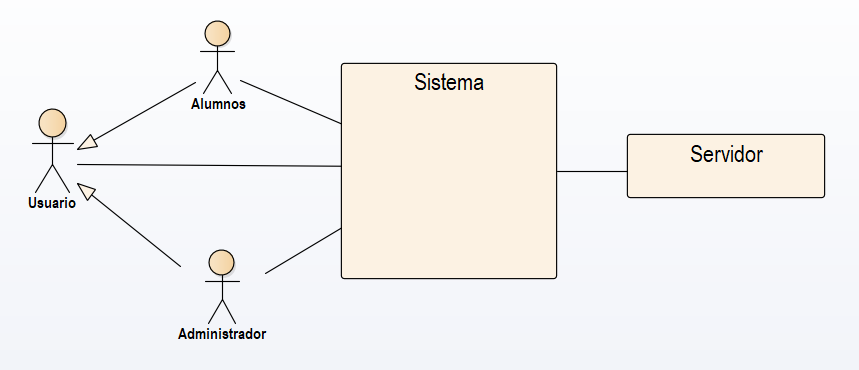
\includegraphics[width=1\textwidth]{imagenes/analisis/diagrama-contexto.png}
        %%Me parece que queda mejor sin el hfill
        %\hfill
    %\caption{epígrafe}
	\label{fig:casos-de-uso}
\end{figure}

\section{Diagramas de Casos de Uso}

Primeramente se muestra un diagrama de caso de uso general donde se agruparon los casos de uso por las acciones en común, luego se va a explorar cada caso de uso de manera mas descriptiva.

Por ejemplo, en ``Gestión de Registros'' van a estar todos los casos de uso referidos a los mismos (alta, baja, listar, buscar, etc)

\subsection{Diagrama de Casos de Uso general}

\begin{figure}[H]
  \centering
    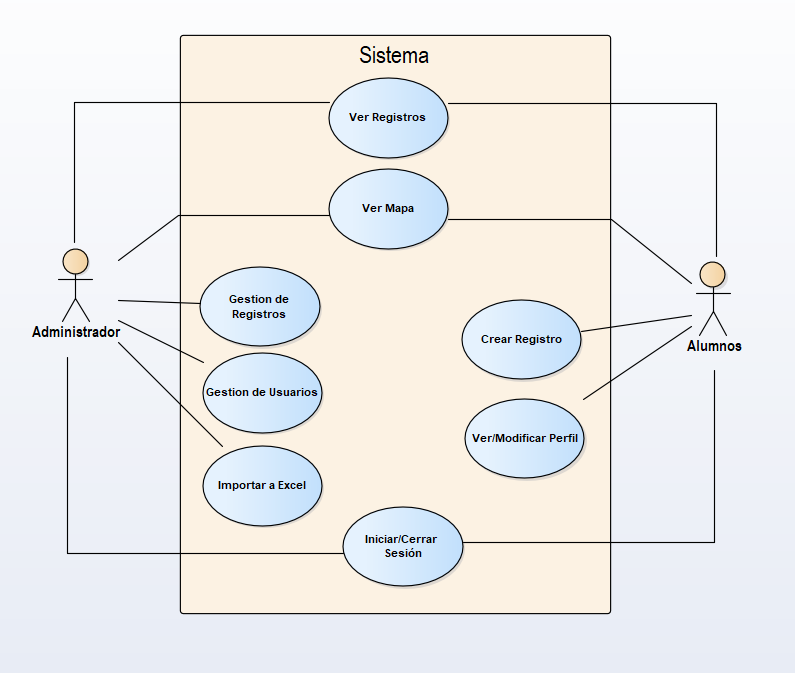
\includegraphics[width=0.7\textwidth]{imagenes/analisis/casos-uso-general.png}
        %%Me parece que queda mejor sin el hfill
        %\hfill
	%\caption{epígrafe}
	\label{fig:casos-de-uso}
\end{figure}

\subsection{Diagrama de Casos de Uso de Gestión de Usuarios}

\begin{figure}[H]
  \centering
    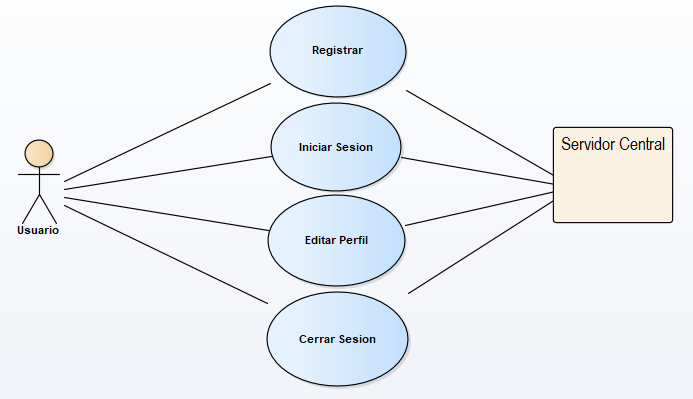
\includegraphics[width=0.7\textwidth]{imagenes/analisis/casos-uso-usuario.png}
        %%Me parece que queda mejor sin el hfill
        %\hfill
    %\caption{epígrafe}
	\label{fig:casos-de-uso-usuario}
\end{figure}

\subsection{Diagrama de Casos de Uso de Gestión de Registros}

\begin{figure}[H]
  \centering
    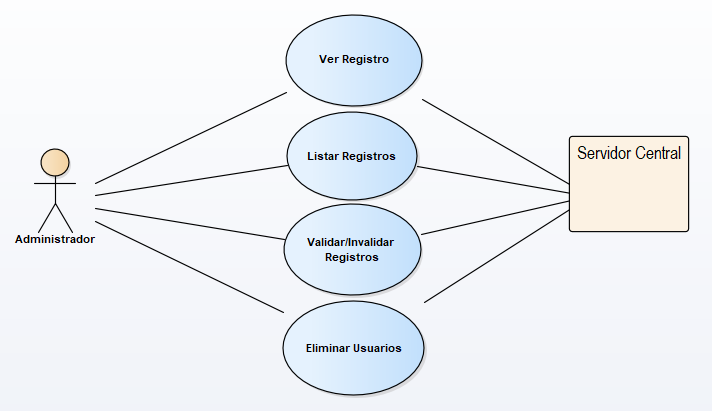
\includegraphics[width=0.7\textwidth]{imagenes/analisis/casos-uso-registros.png}
        %%Me parece que queda mejor sin el hfill
        %\hfill
    %\caption{epígrafe}
    \label{fig:casos-de-uso-tienda}
\end{figure}


\section{Diagramas de Actividad}

\subsection{Inicio de Sesión}
\begin{figure}[H]
  \centering
    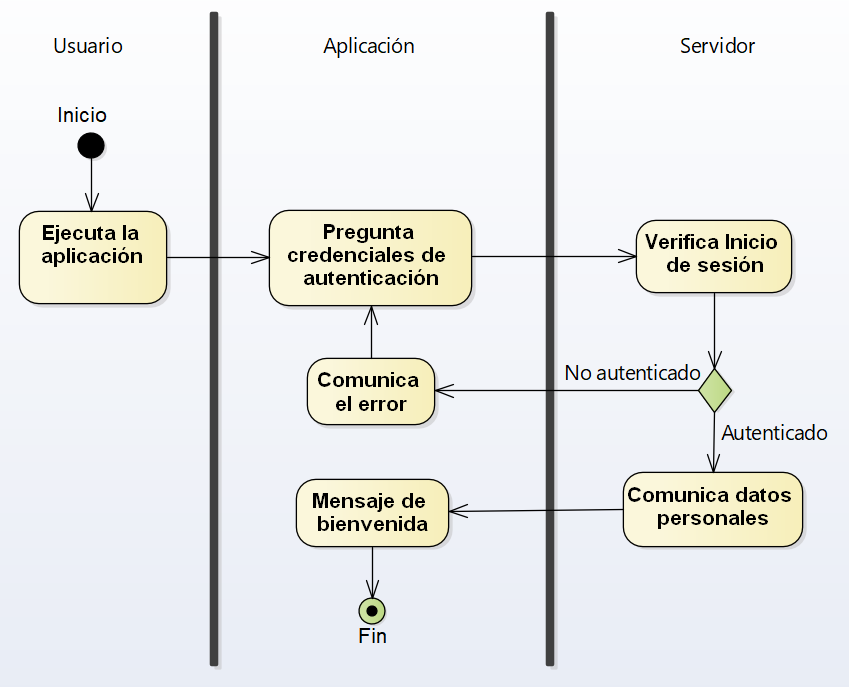
\includegraphics[width=1\textwidth]{imagenes/analisis/diagrama-actividad-inicioSesion.png}
        %%Me parece que queda mejor sin el hfill 
        %\hfill
    \label{fig:diagrama-actividad-autenticar}
\end{figure}

\subsection{Registrar Usuario}

\begin{figure}[H]
  \centering
    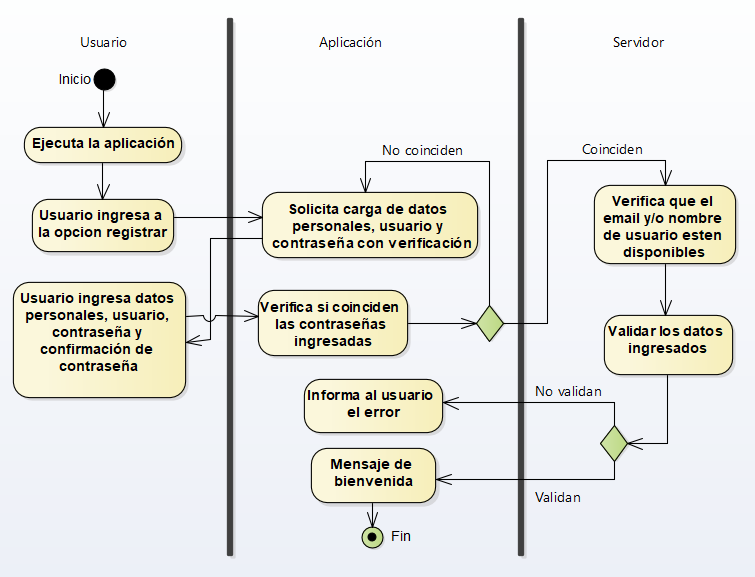
\includegraphics[width=1\textwidth]{imagenes/analisis/diagrama-actividad-registrar.png}
        %%Me parece que queda mejor sin el hfill
        %\hfill 
	\label{fig:diagrama-actividad-registrar}
\end{figure}

\subsection{Crear Registro }

\begin{figure}[H]
  \centering
    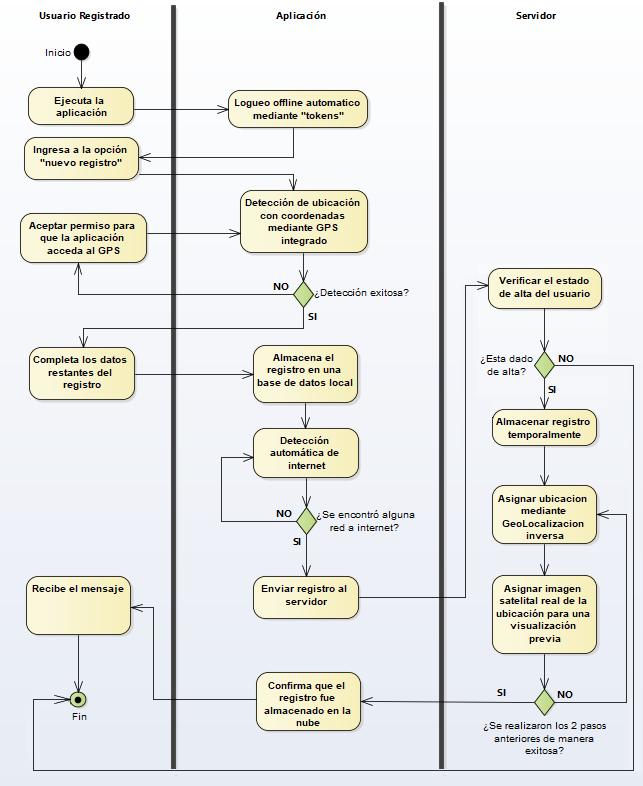
\includegraphics{imagenes/analisis/diagrama-actividad-crear-registro.png}
        %%Me parece que queda mejor sin el hfill
        %\hfill
    \label{fig:diagrama-actividad-crear-tienda}
\end{figure}

\subsection{Ver Mapa Interactivo}

\begin{figure}[H]
  \centering
    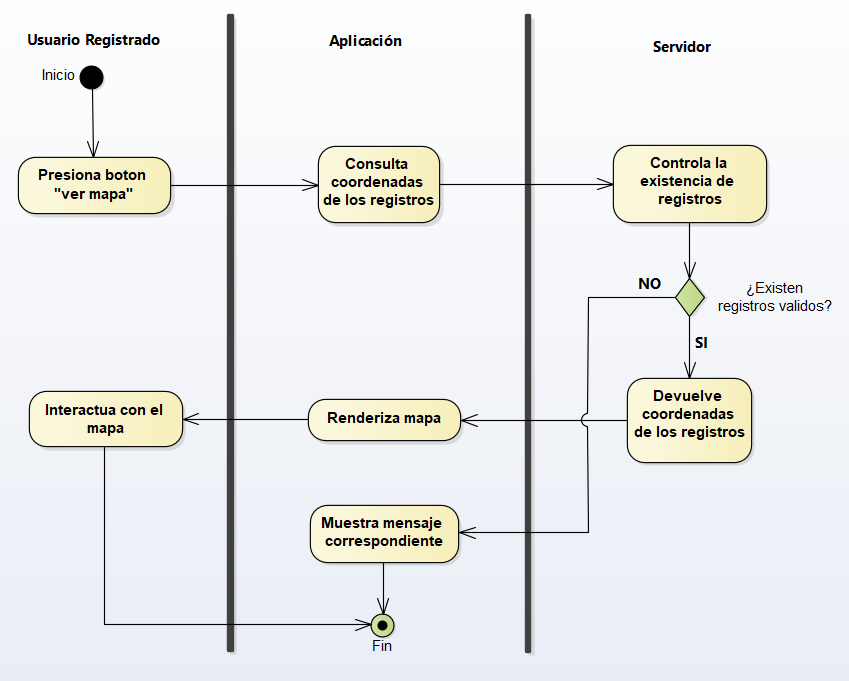
\includegraphics[width=1\textwidth]{imagenes/analisis/diagrama-actividad-ver-mapa.png}
        %%Me parece que queda mejor sin el hfill
        %\hfill
    \label{fig:diagrama-actividad-comprar-producto}
\end{figure}

%% Disciplina de Diseño
%%%%%%%%%%%%%%%%%%%%%%%%%%%%%%%%%%%%%%%%%%%%%%%%%%%%%%%%
%   |------------------------------------------|       %
%   | Web App embebida en dispositivos móviles |       %
%   |  para la gestión de registros sobre la   |       %
%   |   contaminación de afluentes y ríos.     |       %
%   |                                          |       %
%   |          Proyecto de graduación          |       %
%   |__________________________________________|       %
%                                                      %
%   Autores                                            %
%   -------                                            %
%                                                      %
% * Bruno, Ricardo Hugo (CX 1409686)                   %
%     rburnount@gmail.com                              %
% * Gomez Veliz, Kevin Shionen (CX 1411828)            %
%     ing.gomezvelizkevin@gmail.com                    %
%                                                      %
%   Tutor                                              %
%   -------                                            %
%                                                      %
% * Ing. Cohen, Daniel Eduardo                         %
%        dcohen.tuc@gmail.com                          %
%                                                      %
%   Cotutor                                            %
%   -------                                            %
%                                                      %
% * Ing. Nieto, Luis Eduardo                           %
%        lnieto@herrera.unt.edu.ar                     %
%                                                      %
%                                                      %
%%%%%%%%%%%%%%%%%%%%%%%%%%%%%%%%%%%%%%%%%%%%%%%%%%%%%%%%

\chapter{Disciplina de Diseño}
\label{chap:disenio}

Por el Principio de Pareto\footnote{Cuando se habla de los costes de desarrollo de software enunciarse de la siguiente manera: ``El 80\% del esfuerzo de desarrollo (en tiempo y recursos) produce el 20\% del código, mientras que el 80\% restante es producido con tan sólo un 20\% del esfuerzo''}, se hicieron los diagramas relevantes. Como se procura tener homogeneidad en la implementación de las clases, basta un solo diagrama de cada tipo para una clase, para describir también el comportamiento de las otras clases.
    

\section{Descripción Textual de Casos de Uso}

%#############################################################################
%#   
%#   Caso de uso 1
%#
%#############################################################################

\subsection{Caso de Uso 01: Un alumno no registrado desea registrarse en el sistema.}

\begin{longtable}{|l|p{5.5cm}|l|p{2cm}|l|p{1.9cm}|} \hline
    \cellcolor{grisOscuro} CU01 & \multicolumn{4}{|l|}{  \cellcolor{grisOscuro} Registrar} &  \cellcolor{grisClaro}\multirow{2}{1cm}{} \\ \cline{1-5}
    \cellcolor{grisOscuro} Revisa: &  \cellcolor{grisClaro} &  \cellcolor{grisOscuro} Fecha &  \cellcolor{grisClaro} &  \cellcolor{grisOscuro} Firma: & \cellcolor{grisClaro} \\ \hline
    \multicolumn{6}{|p{15cm}|}{ \textbf{Resumen: } Este caso de uso permite a los usuarios registrarse como usuarios de la aplicación, permitiendo introducir sus datos personales

    } \\ \hline

    \multicolumn{6}{|p{15cm}|}{ \textbf{Actores: } Usuario (primario). Servidor (en adelante S. Secundario)

    } \\ \hline

    \multicolumn{6}{|p{15cm}|}{ \textbf{Personal Involucrado y Metas: }
    
    \emph{Usuario:} quiere transformarse en un usuario del sistema, así pueda realizar las transacciones con la aplicación de un modo seguro y personalizado.
    
    \emph{Servidor: } quiere registrar la mayor cantidad de usuarios posibles y que el proceso sea lo más rápido y seguro posible.
    } \\ \hline

    \multicolumn{6}{|p{15cm}|}{ \textbf{Precondiciones: } El usuario no está registrado en la aplicación

    } \\ \hline

    \multicolumn{6}{|p{15cm}|}{ \textbf{Poscondiciones: } Se registra al usuario como usuario de la aplicación. El usuario puede realizar operaciones en la aplicación.

    } \\ \hline

    \multicolumn{6}{|p{15cm}|}{ \textbf{Escenario Principal: }
        \begin{enumerate}
            \item El usuario ejecuta la aplicación móvil (en adelante APP) en su SmartPhone y decide registrarse.
            \item APP muestra un formulario de carga donde ingresa sus datos personales y su nombre de usuario y contraseña.
            \item APP verifica los datos ingresados.
            \item APP solicita a S el registro del usuario.
            \item S registra al usuario y lo informa a APP.
            \item APP da la bienvenida al usuario.
        \end{enumerate}

    } \\ \hline

    \multicolumn{6}{|p{15cm}|}{ \textbf{Flujos Alternativos: }

    \textbf{A1: El sistema encuentra algún fallo para comunicarse con S}

    La secuencia A1 comienza en el punto 4 del escenario principal.
    \begin{enumerate}
        \setcounter{enumi}{4}
        \item APP informa al usuario el problema de conexión a través de un mensaje por la pantalla.
    \end{enumerate}

    El escenario vuelve al punto 4.

    \textbf{A2: Nombre de usuario existente}
    
    La secuencia A2 comienza en el punto 4 del escenario principal.
    \begin{enumerate}
        \setcounter{enumi}{4}
        \item S comunica que el nombre de usuario es existente.
    \end{enumerate}

    El escenario vuelve al punto 3.

    \textbf{A3: Contraseña inválida o no coincide con la confirmación}
    
    La secuencia A3 comienza en el punto 3 del escenario principal.
    \begin{enumerate}
        \setcounter{enumi}{3}
        \item APP informa el problema a través de un mensaje por pantalla.
    \end{enumerate}

    El escenario vuelve al punto 2.

    \textbf{A4: Dirección de correo electrónico existente}
    
    La secuencia A4 comienza en el punto 4 del escenario principal.
    \begin{enumerate}
        \setcounter{enumi}{4}
        \item S comunica que la dirección de correo electrónico es existente.
    \end{enumerate}

    El escenario vuelve al punto 2.

    \textbf{A5: Tipo de datos ingresados de manera incorrecta}
    
    La secuencia A5 comienza en el punto 3 del escenario principal.
    \begin{enumerate}
        \setcounter{enumi}{3}
        \item APP informa el problema a través de un mensaje por pantalla.
    \end{enumerate}

    El escenario vuelve al punto 2.

    } \\ \hline

    \multicolumn{6}{|p{15cm}|}{ \textbf{Requisitos de Interfaz de Usuario para todos los casos de uso: }

    SmartPhone con SO Android o iOS o Windows Mobile, con pantalla táctil, cámara y GPS integrado.
    
    } \\ \hline

    \multicolumn{6}{|p{15cm}|}{ \textbf{Requisitos No-Funcionales para todos los casos de uso: }

    \emph{Tiempo de respuesta:} la interfaz debe responder dentro de un tiempo máximo de 3 segundos en una velocidad efectiva de conexión con el servidor a través de 3G.

    \emph{Disponibilidad:} debe poder accederse a toda hora, los 365 días del año. asdadasdasdasd

    } \\ \hline

\end{longtable}



%#############################################################################
%#   
%#   Caso de uso 2
%#
%#############################################################################

\subsection{Caso de Uso UC2: Un alumno registrado desea iniciar sesión.}

\begin{longtable}{|l|p{5.5cm}|l|p{2cm}|l|p{1.9cm}|} \hline
    \cellcolor{grisOscuro} CU02 & \multicolumn{4}{|l|}{  \cellcolor{grisOscuro} Iniciar Sesión} &  \cellcolor{grisClaro}\multirow{2}{1cm}{} \\ \cline{1-5}
    \cellcolor{grisOscuro} Revisa: &  \cellcolor{grisClaro} &  \cellcolor{grisOscuro} Fecha &  \cellcolor{grisClaro} &  \cellcolor{grisOscuro} Firma: & \cellcolor{grisClaro} \\ \hline
    \multicolumn{6}{|p{15cm}|}{ \textbf{Resumen: } Este caso de uso permite a los usuarios iniciar sesión con el nombre de usuario y contraseña de manera que el sistema le permita realizar tareas.

    } \\ \hline

    \multicolumn{6}{|p{15cm}|}{ \textbf{Actores: } Usuario (Primario). Servidor (en adelante S. Secundario)

    } \\ \hline

    \multicolumn{6}{|p{15cm}|}{ \textbf{Personal Involucrado y Metas: }

    \emph{Usuario:} quiere que el sistema lo reconozca como tal, así pueda realizar las tareas con la aplicación de un modo seguro y personalizado.

    \emph{Servidor:} requiere identificar confiablemente a sus usuarios de manera de satisfacer sus intereses en cuando a seguridad, accesos a su cuenta personal y datos privados.

    } \\ \hline

    \multicolumn{6}{|p{15cm}|}{ \textbf{Precondiciones: } El usuario está registrado.

    } \\ \hline

    \multicolumn{6}{|p{15cm}|}{ \textbf{Poscondiciones: } Se identifica y autentica al usuario. Se conocen sus datos personales y opciones de personalización.

    } \\ \hline

    \multicolumn{6}{|p{15cm}|}{ \textbf{Escenario Principal: }

    \begin{enumerate}
        \item El usuario ejecuta la aplicación móvil (en adelante APP) en su SmartPhone.
        \item APP solicita al usuario su nombre de usuario y contraseña.
        \item El usuario ingresa su nombre de usuario y contraseña.
        \item APP solicita a S la validación del usuario
        \item S valida al usuario y comunica sus datos personales.
        \item APP da la bienvenida al usuario
    \end{enumerate}

    } \\ \hline

    \multicolumn{6}{|p{15cm}|}{ \textbf{Flujos Alternativos: }

    \textbf{A1: El sistema encuentra algún fallo para comunicarse con S}
    
    La secuencia A1 comienza en el punto 4 del escenario principal.
    \begin{enumerate}
        \setcounter{enumi}{4}
        \item APP informa al usuario el problema de conexión a través de un mensaje por la pantalla.
    \end{enumerate}

    El escenario vuelve al punto 2.

    \textbf{A2: Nombre de usuario inexistente}
    
    La secuencia A2 comienza en el punto 4 del escenario principal.
    \begin{enumerate}
        \setcounter{enumi}{4}
        \item S comunica que el nombre de usuario es inexistente.
    \end{enumerate}

    El escenario vuelve al punto 2.

    \textbf{A3: Nombre de usuario existente pero contraseña inválida}
    
    La secuencia A3 comienza en el punto 4 del escenario principal.
    \begin{enumerate}
        \setcounter{enumi}{3}
        \item S comunica que la contraseña es inválida.
    \end{enumerate}

    El escenario vuelve al punto 2.

    } \\ \hline

\end{longtable}

%#############################################################################
%#   
%#   Caso de uso 3
%#
%#############################################################################

\subsection{Caso de Uso UC3: Crear Tienda}

\begin{longtable}{|l|p{5.5cm}|l|p{2cm}|l|p{1.9cm}|} \hline
    \cellcolor{grisOscuro} CU01 & \multicolumn{4}{|l|}{  \cellcolor{grisOscuro} Registrar} &  \cellcolor{grisClaro}\multirow{2}{1cm}{} \\ \cline{1-5}
    \cellcolor{grisOscuro} Revisa: &  \cellcolor{grisClaro} &  \cellcolor{grisOscuro} Fecha &  \cellcolor{grisClaro} &  \cellcolor{grisOscuro} Firma: & \cellcolor{grisClaro} \\ \hline
    \multicolumn{6}{|p{15cm}|}{ \textbf{Resumen: } En

    } \\ \hline

    \multicolumn{6}{|p{15cm}|}{ \textbf{Actores: }

    } \\ \hline

    \multicolumn{6}{|p{15cm}|}{ \textbf{Personal Involucrado y Metas: }

    } \\ \hline

    \multicolumn{6}{|p{15cm}|}{ \textbf{Precondiciones: }

    } \\ \hline

    \multicolumn{6}{|p{15cm}|}{ \textbf{Poscondiciones: }

    } \\ \hline

    \multicolumn{6}{|p{15cm}|}{ \textbf{Escenario Principal: }

    } \\ \hline

    \multicolumn{6}{|p{15cm}|}{ \textbf{Flujos Alternativos: }

    } \\ \hline

\end{longtable}

\begin{framed}

%\noindent\hline

\subsubsection{Resumen:} Este caso de uso permite al vendedor crear una tienda de manera que el sistema le permita realizar transacciones y operaciones sobre sus productos.


\subsubsection{Actores:} Vendedor (primario). S (secundario)

\subsubsection{Personal Involucrado y Metas:}

\emph{Vendedor:} quiere que el sistema lo reconozca como tal, así pueda realizar las transacciones a través del sitio, y la administración de sus productos de un modo seguro y personalizado.

\emph{Servidor:} requiere identificar confiablemente a sus usuarios vendedores de manera de satisfacer sus intereses en cuanto a seguridad, productos publicados y datos privados. 

\subsubsection{Precondiciones:} 
Los usuarios deben estar autenticados en AM. 

\subsubsection{Poscondiciones:} 
Se registra una nueva tienda en el sistema con los datos básicos necesarios para realizar ventas.

\subsubsection{Escenario Principal: }

\begin{enumerate}
    \item El vendedor selecciona la opción para crear tienda. 
    \item AM solicita al vendedor a través de un formulario los datos básicos requeridos para la creación de la tienda.
    \item El vendedor completa el formulario y presiona un botón para finalizar.
    \item AM envía de manera segura los datos a S para que sean validados.
    \item S valida los datos, realiza la creación la tienda y envía una confirmación.
    \item AM informa al usuario que la operación se realizó exitosamente.
\end{enumerate}

\subsubsection{Flujos Alternativos: }

%El  comando alternativo está definido en el documento principal. Es un paragraph con salto de línea
\alternativo{A1:el sistema encuentra algún fallo para comunicarse con S}
La secuencia A1 comienza en el punto 4 del escenario principal. 
\begin{enumerate}
    %Comienza a partir del 5° item
    \setcounter{enumi}{4}
    \item AM informa al usuario el problema de conexión a través de un mensaje por la pantalla.
\end{enumerate}
El escenario vuelve al punto 4.

%}}
\end{framed}

%#############################################################################
%#   
%#   Caso de uso 4
%#
%#############################################################################

\subsection{Caso de Uso UC4: Editar Tienda}

\begin{longtable}{|l|p{5.5cm}|l|p{2cm}|l|p{1.9cm}|} \hline
    \cellcolor{grisOscuro} CU01 & \multicolumn{4}{|l|}{  \cellcolor{grisOscuro} Registrar} &  \cellcolor{grisClaro}\multirow{2}{1cm}{} \\ \cline{1-5}
    \cellcolor{grisOscuro} Revisa: &  \cellcolor{grisClaro} &  \cellcolor{grisOscuro} Fecha &  \cellcolor{grisClaro} &  \cellcolor{grisOscuro} Firma: & \cellcolor{grisClaro} \\ \hline
    \multicolumn{6}{|p{15cm}|}{ \textbf{Resumen: } En

    } \\ \hline

    \multicolumn{6}{|p{15cm}|}{ \textbf{Actores: }

    } \\ \hline

    \multicolumn{6}{|p{15cm}|}{ \textbf{Personal Involucrado y Metas: }

    } \\ \hline

    \multicolumn{6}{|p{15cm}|}{ \textbf{Precondiciones: }

    } \\ \hline

    \multicolumn{6}{|p{15cm}|}{ \textbf{Poscondiciones: }

    } \\ \hline

    \multicolumn{6}{|p{15cm}|}{ \textbf{Escenario Principal: }

    } \\ \hline

    \multicolumn{6}{|p{15cm}|}{ \textbf{Flujos Alternativos: }

    } \\ \hline

\end{longtable}

\begin{framed}

%\noindent\hline

\subsubsection{Resumen:} Este caso de uso permite al vendedor editar los datos de su tienda.


\subsubsection{Actores:} Vendedor (primario). S (secundario)

\subsubsection{Personal Involucrado y Metas:}

\emph{Vendedor:} quiere editar los datos de su tienda.

\emph{Servidor:} requiere mantener actualizados los datos del vendedor.

\subsubsection{Precondiciones:} 
El vendedor debe estar autenticado en AM. 

\subsubsection{Poscondiciones:} 
Se registran los cambios de los datos de la tienda en el servidor.

\subsubsection{Escenario Principal: }

\begin{enumerate}
    \item El vendedor selecciona la opción para editar tienda. 
    \item AM solicita al vendedor a través de un formulario los datos de la tienda que pueden ser modificados o mantenidos.
    \item El vendedor completa el formulario y presiona un botón para finalizar.
    \item AM envía de manera segura los datos a S para que sean validados.
    \item S valida los datos, realiza la actualización y envía una confirmación.
    \item AM informa al usuario que la operación se realizó exitosamente.
\end{enumerate}

\subsubsection{Flujos Alternativos: }

%El  comando alternativo está definido en el documento principal. Es un paragraph con salto de línea
\alternativo{A1:El sistema encuentra algún fallo para comunicarse con S}
La secuencia A1 comienza en el punto 4 del escenario principal.
\begin{enumerate}
    %Comienza a partir del 5° item
    \setcounter{enumi}{4}
    \item AM informa al usuario el problema de conexión a través de un mensaje por la pantalla.
\end{enumerate}
El escenario vuelve al punto 4.

%}}
\end{framed}

%#############################################################################
%#   
%#   Caso de uso 5
%#
%#############################################################################

\subsection{Caso de Uso UC5: Editar Perfil}

\begin{longtable}{|l|p{5.5cm}|l|p{2cm}|l|p{1.9cm}|} \hline
    \cellcolor{grisOscuro} CU01 & \multicolumn{4}{|l|}{  \cellcolor{grisOscuro} Registrar} &  \cellcolor{grisClaro}\multirow{2}{1cm}{} \\ \cline{1-5}
    \cellcolor{grisOscuro} Revisa: &  \cellcolor{grisClaro} &  \cellcolor{grisOscuro} Fecha &  \cellcolor{grisClaro} &  \cellcolor{grisOscuro} Firma: & \cellcolor{grisClaro} \\ \hline
    \multicolumn{6}{|p{15cm}|}{ \textbf{Resumen: } En

    } \\ \hline

    \multicolumn{6}{|p{15cm}|}{ \textbf{Actores: }

    } \\ \hline

    \multicolumn{6}{|p{15cm}|}{ \textbf{Personal Involucrado y Metas: }

    } \\ \hline

    \multicolumn{6}{|p{15cm}|}{ \textbf{Precondiciones: }

    } \\ \hline

    \multicolumn{6}{|p{15cm}|}{ \textbf{Poscondiciones: }

    } \\ \hline

    \multicolumn{6}{|p{15cm}|}{ \textbf{Escenario Principal: }

    } \\ \hline

    \multicolumn{6}{|p{15cm}|}{ \textbf{Flujos Alternativos: }

    } \\ \hline

\end{longtable}


\begin{framed}

%\noindent\hline

\subsubsection{Resumen:} Este caso de uso permite al usuario editar los datos de su perfil.


\subsubsection{Actores:} Usuario(primario). S (secundario)

\subsubsection{Personal Involucrado y Metas:}

\emph{Usuario:} quiere editar los datos de su perfil.

\emph{Servidor:} requiere mantener actualizados los datos del usuario.

\subsubsection{Precondiciones:} 
El usuario debe estar autenticado en AM. 

\subsubsection{Poscondiciones:} 
Se registran los cambios de los datos de perfil en el servidor.

\subsubsection{Escenario Principal: }

\begin{enumerate}
    \item El usuario selecciona la opción para editar perfil. 
    \item AM solicita al usuario a través de un formulario los datos del perfil de usuario que pueden ser modificados o mantenidos.
    \item El usuario completa el formulario y presiona un botón para finalizar.
    \item AM envía de manera segura los datos a S para que sean validados.
    \item S valida los datos, realiza la actualización y envía una confirmación.
    \item AM informa al usuario que la operación se realizó exitosamente.
\end{enumerate}

\subsubsection{Flujos Alternativos: }

%El  comando alternativo está definido en el documento principal. Es un paragraph con salto de línea
\alternativo{A1:el sistema encuentra algún fallo para comunicarse con S}
La secuencia A1 comienza en el punto 4 del escenario principal.
\begin{enumerate}
    %Comienza a partir del 5° item
    \setcounter{enumi}{4}
    \item AM informa al usuario el problema de conexión a través de un mensaje por la pantalla.
\end{enumerate}
El escenario vuelve al punto 4.

%}}
\end{framed}

%#############################################################################
%#   
%#   Caso de uso 6
%#
%#############################################################################

\subsection{Caso de Uso UC6: Crear Producto}

\begin{longtable}{|l|p{5.5cm}|l|p{2cm}|l|p{1.9cm}|} \hline
    \cellcolor{grisOscuro} CU01 & \multicolumn{4}{|l|}{  \cellcolor{grisOscuro} Registrar} &  \cellcolor{grisClaro}\multirow{2}{1cm}{} \\ \cline{1-5}
    \cellcolor{grisOscuro} Revisa: &  \cellcolor{grisClaro} &  \cellcolor{grisOscuro} Fecha &  \cellcolor{grisClaro} &  \cellcolor{grisOscuro} Firma: & \cellcolor{grisClaro} \\ \hline
    \multicolumn{6}{|p{15cm}|}{ \textbf{Resumen: } En

    } \\ \hline

    \multicolumn{6}{|p{15cm}|}{ \textbf{Actores: }

    } \\ \hline

    \multicolumn{6}{|p{15cm}|}{ \textbf{Personal Involucrado y Metas: }

    } \\ \hline

    \multicolumn{6}{|p{15cm}|}{ \textbf{Precondiciones: }

    } \\ \hline

    \multicolumn{6}{|p{15cm}|}{ \textbf{Poscondiciones: }

    } \\ \hline

    \multicolumn{6}{|p{15cm}|}{ \textbf{Escenario Principal: }

    } \\ \hline

    \multicolumn{6}{|p{15cm}|}{ \textbf{Flujos Alternativos: }

    } \\ \hline

\end{longtable}


\begin{framed}

%\noindent\hline

\subsubsection{Resumen:} Este caso de uso permite al vendedor crear un producto de manera que el sistema le permita ofrecerlo a la venta.


\subsubsection{Actores:} Vendedor (primario). S (secundario)

\subsubsection{Personal Involucrado y Metas:}

\emph{Vendedor:} quiere ofrecer sus productos a través del sistema.

\emph{Servidor:} requiere obtener la información de los  productos de manera que sea posible ofrecérselo a los compradores.

\subsubsection{Precondiciones:} 
El vendedor debe estar autenticados en AM. 

\subsubsection{Poscondiciones:} 
Se crea un nuevo producto en el sistema.

\subsubsection{Escenario Principal: }

\begin{enumerate}
    \item El vendedor selecciona la opción para crear producto. 
    \item AM solicita al vendedor a través de un formulario los datos básicos requeridos para la creación del producto.
    \item El vendedor completa el formulario y presiona un botón para finalizar.
    \item AM envía de manera segura los datos a S para que sean validados.
    \item S valida los datos, realiza la creación del producto y envía una confirmación.
    \item AM informa al usuario que la operación se realizó exitosamente.
\end{enumerate}

\subsubsection{Flujos Alternativos: }

%El  comando alternativo está definido en el documento principal. Es un paragraph con salto de línea
\alternativo{A1:el sistema encuentra algún fallo para comunicarse con S}
La secuencia A1 comienza en el punto 4 del escenario principal.
\begin{enumerate}
    %Comienza a partir del 5° item
    \setcounter{enumi}{4}
    \item AM informa al vendedor el problema de conexión a través de un mensaje por la pantalla.
\end{enumerate}
El escenario vuelve al punto 4.

%}}
\end{framed}

%#############################################################################
%#   
%#   Caso de uso 7
%#
%#############################################################################

\subsection{Caso de Uso UC7: Editar Producto}

\begin{longtable}{|l|p{5.5cm}|l|p{2cm}|l|p{1.9cm}|} \hline
    \cellcolor{grisOscuro} CU01 & \multicolumn{4}{|l|}{  \cellcolor{grisOscuro} Registrar} &  \cellcolor{grisClaro}\multirow{2}{1cm}{} \\ \cline{1-5}
    \cellcolor{grisOscuro} Revisa: &  \cellcolor{grisClaro} &  \cellcolor{grisOscuro} Fecha &  \cellcolor{grisClaro} &  \cellcolor{grisOscuro} Firma: & \cellcolor{grisClaro} \\ \hline
    \multicolumn{6}{|p{15cm}|}{ \textbf{Resumen: } En

    } \\ \hline

    \multicolumn{6}{|p{15cm}|}{ \textbf{Actores: }

    } \\ \hline

    \multicolumn{6}{|p{15cm}|}{ \textbf{Personal Involucrado y Metas: }

    } \\ \hline

    \multicolumn{6}{|p{15cm}|}{ \textbf{Precondiciones: }

    } \\ \hline

    \multicolumn{6}{|p{15cm}|}{ \textbf{Poscondiciones: }

    } \\ \hline

    \multicolumn{6}{|p{15cm}|}{ \textbf{Escenario Principal: }

    } \\ \hline

    \multicolumn{6}{|p{15cm}|}{ \textbf{Flujos Alternativos: }

    } \\ \hline

\end{longtable}

\begin{framed}

%\noindent\hline

\subsubsection{Resumen:} Este caso de uso permite al vendedor editar los datos de uno de sus productos.


\subsubsection{Actores:} Vendedor (primario). S (secundario)

\subsubsection{Personal Involucrado y Metas:}

\emph{Vendedor:} quiere ofrecer sus productos a través del sistema.

\emph{Servidor:} requiere obtener la información de los  productos de manera que sea posible ofrecérselo a los compradores.

\subsubsection{Precondiciones:} 
El vendedor debe estar autenticados en AM. 

\subsubsection{Poscondiciones:} 
Se registran los cambios de los datos del producto en el servidor.

\subsubsection{Escenario Principal: }

\begin{enumerate}
    \item El vendedor selecciona la opción para editar producto. 
    \item AM solicita al vendedor a través de un formulario los datos del producto que pueden ser modificados o mantenidos.
    \item El vendedor completa el formulario y presiona un botón para finalizar.
    \item AM envía de manera segura los datos a S para que sean validados.
    \item S valida los datos, realiza la actualización y envía una confirmación.
    \item AM informa al usuario que la operación se realizó exitosamente.
\end{enumerate}

\subsubsection{Flujos Alternativos: }

%El  comando alternativo está definido en el documento principal. Es un paragraph con salto de línea
\alternativo{A1:el sistema encuentra algún fallo para comunicarse con S}
La secuencia A1 comienza en el punto 4 del escenario principal.
\begin{enumerate}
    %Comienza a partir del 5° item
    \setcounter{enumi}{4}
    \item AM informa al vendedor el problema de conexión a través de un mensaje por la pantalla.
\end{enumerate}
El escenario vuelve al punto 4.

%}}
\end{framed}

%#############################################################################
%#   
%#   Caso de uso 8
%#
%#############################################################################

\subsection{Caso de Uso UC8: Eliminar Producto}

\begin{longtable}{|l|p{5.5cm}|l|p{2cm}|l|p{1.9cm}|} \hline
    \cellcolor{grisOscuro} CU01 & \multicolumn{4}{|l|}{  \cellcolor{grisOscuro} Registrar} &  \cellcolor{grisClaro}\multirow{2}{1cm}{} \\ \cline{1-5}
    \cellcolor{grisOscuro} Revisa: &  \cellcolor{grisClaro} &  \cellcolor{grisOscuro} Fecha &  \cellcolor{grisClaro} &  \cellcolor{grisOscuro} Firma: & \cellcolor{grisClaro} \\ \hline
    \multicolumn{6}{|p{15cm}|}{ \textbf{Resumen: } En

    } \\ \hline

    \multicolumn{6}{|p{15cm}|}{ \textbf{Actores: }

    } \\ \hline

    \multicolumn{6}{|p{15cm}|}{ \textbf{Personal Involucrado y Metas: }

    } \\ \hline

    \multicolumn{6}{|p{15cm}|}{ \textbf{Precondiciones: }

    } \\ \hline

    \multicolumn{6}{|p{15cm}|}{ \textbf{Poscondiciones: }

    } \\ \hline

    \multicolumn{6}{|p{15cm}|}{ \textbf{Escenario Principal: }

    } \\ \hline

    \multicolumn{6}{|p{15cm}|}{ \textbf{Flujos Alternativos: }

    } \\ \hline

\end{longtable}

\begin{framed}

%\noindent\hline

\subsubsection{Resumen:} Este caso de uso permite al vendedor eliminar un producto de la tienda.


\subsubsection{Actores:} Vendedor (primario). S (secundario)

\subsubsection{Personal Involucrado y Metas:}

\emph{Vendedor:} quiere eliminar un producto de su tienda.

\emph{Servidor:} elimina al producto.

\subsubsection{Precondiciones:} 
El vendedor debe estar autenticados en AM. 

\subsubsection{Poscondiciones:} 
Se elimina el producto de la tienda.

\subsubsection{Escenario Principal: }

\begin{enumerate}
    \item El vendedor selecciona la opción para eliminar el producto. 
    \item AM solicita al vendedor que confirme que quiere eliminar el producto.
    \item El vendedor presiona un botón para confirmar.
    \item AM envía de manera segura la solicitud a S para que sean validados.
    \item S valida la solicitud, realiza el cambio de estado en el producto y envía una confirmación.
    \item AM informa al usuario que la operación se realizó exitosamente.
\end{enumerate}

\subsubsection{Flujos Alternativos: }

%El  comando alternativo está definido en el documento principal. Es un paragraph con salto de línea
\alternativo{A1:el sistema encuentra algún fallo para comunicarse con S}
La secuencia A1 comienza en el punto 4 del escenario principal.
\begin{enumerate}
    %Comienza a partir del 5° item
    \setcounter{enumi}{4}
    \item AM informa al vendedor el problema de conexión a través de un mensaje por la pantalla.
\end{enumerate}
El escenario vuelve al punto 4.

%}}
\end{framed}

%#############################################################################
%#   
%#   Caso de uso 9
%#
%#############################################################################

\subsection{Caso de Uso UC9: Buscar Producto}

\begin{longtable}{|l|p{5.5cm}|l|p{2cm}|l|p{1.9cm}|} \hline
    \cellcolor{grisOscuro} CU01 & \multicolumn{4}{|l|}{  \cellcolor{grisOscuro} Registrar} &  \cellcolor{grisClaro}\multirow{2}{1cm}{} \\ \cline{1-5}
    \cellcolor{grisOscuro} Revisa: &  \cellcolor{grisClaro} &  \cellcolor{grisOscuro} Fecha &  \cellcolor{grisClaro} &  \cellcolor{grisOscuro} Firma: & \cellcolor{grisClaro} \\ \hline
    \multicolumn{6}{|p{15cm}|}{ \textbf{Resumen: } En

    } \\ \hline

    \multicolumn{6}{|p{15cm}|}{ \textbf{Actores: }

    } \\ \hline

    \multicolumn{6}{|p{15cm}|}{ \textbf{Personal Involucrado y Metas: }

    } \\ \hline

    \multicolumn{6}{|p{15cm}|}{ \textbf{Precondiciones: }

    } \\ \hline

    \multicolumn{6}{|p{15cm}|}{ \textbf{Poscondiciones: }

    } \\ \hline

    \multicolumn{6}{|p{15cm}|}{ \textbf{Escenario Principal: }

    } \\ \hline

    \multicolumn{6}{|p{15cm}|}{ \textbf{Flujos Alternativos: }

    } \\ \hline

\end{longtable}



\begin{framed}

%\noindent\hline

\subsubsection{Resumen:} Este caso de uso permite a un usuario realizar una búsqueda de productos.


\subsubsection{Actores:} Usuario (primario). S (secundario)

\subsubsection{Personal Involucrado y Metas:}

\emph{Usuario:} quiere obtener los productos que coincidan con un determinado criterio de búsqueda

\emph{Servidor:} quiere ofrecer al usuario los productos que mejor se ajustan a su búsqueda.

\subsubsection{Poscondiciones:} 
Se obtiene un listado de productos que cumplen con la condición de búsqueda.

\subsubsection{Escenario Principal: }

\begin{enumerate}
    \item El usuario ingresa el texto que se buscará.  
    \item El usuario presiona un botón para comenzar la búsqueda.
    \item AM envía la solicitud de búsqueda a S
    \item S verifica los productos que cumplen con el criterio buscado
    \item S retorna el listado de productos
    \item AM muestra el listado al usuario
\end{enumerate}

\subsubsection{Flujos Alternativos: }

%El  comando alternativo está definido en el documento principal. Es un paragraph con salto de línea
\alternativo{A1:el sistema encuentra algún fallo para comunicarse con S}
La secuencia A1 comienza en el punto 3 del escenario principal.
\begin{enumerate}
    %Comienza a partir del 5° item
    \setcounter{enumi}{4}
    \item AM informa al usuario el problema de conexión a través de un mensaje por la pantalla.
\end{enumerate}
El escenario vuelve al punto 3.

%}}
\end{framed}

%#############################################################################
%#   
%#   Caso de uso 10
%#
%#############################################################################

\subsection{Caso de Uso UC10: Comprar Producto}

\begin{longtable}{|l|p{5.5cm}|l|p{2cm}|l|p{1.9cm}|} \hline
    \cellcolor{grisOscuro} CU01 & \multicolumn{4}{|l|}{  \cellcolor{grisOscuro} Registrar} &  \cellcolor{grisClaro}\multirow{2}{1cm}{} \\ \cline{1-5}
    \cellcolor{grisOscuro} Revisa: &  \cellcolor{grisClaro} &  \cellcolor{grisOscuro} Fecha &  \cellcolor{grisClaro} &  \cellcolor{grisOscuro} Firma: & \cellcolor{grisClaro} \\ \hline
    \multicolumn{6}{|p{15cm}|}{ \textbf{Resumen: } En

    } \\ \hline

    \multicolumn{6}{|p{15cm}|}{ \textbf{Actores: }

    } \\ \hline

    \multicolumn{6}{|p{15cm}|}{ \textbf{Personal Involucrado y Metas: }

    } \\ \hline

    \multicolumn{6}{|p{15cm}|}{ \textbf{Precondiciones: }

    } \\ \hline

    \multicolumn{6}{|p{15cm}|}{ \textbf{Poscondiciones: }

    } \\ \hline

    \multicolumn{6}{|p{15cm}|}{ \textbf{Escenario Principal: }

    } \\ \hline

    \multicolumn{6}{|p{15cm}|}{ \textbf{Flujos Alternativos: }

    } \\ \hline

\end{longtable}

\begin{framed}

%\noindent\hline

\subsubsection{Resumen:} Este caso de uso permite a un comprador realizar la compra de un producto.


\subsubsection{Actores:} Comprador (primario). Vendedor y S (secundarios)

\subsubsection{Personal Involucrado y Metas:}

\emph{Comprador:} quiere realizar la compra del producto en el que está interesado.

\emph{Vendedor:} quiere que la venta se realice sin inconvenientes y de manera sencilla.

\emph{Servidor:} quiere que la operación de compra se realice de manera segura y todos los datos relevantes sean almacenados correctamente.


\subsubsection{Precondiciones:} 
Los usuarios deben estar autenticados en AM.

\subsubsection{Poscondiciones:} 
Se registra la compra

\subsubsection{Escenario Principal: }

\begin{enumerate}
    \item El comprador selecciona la opción para comprar el producto.  
    \item El comprador selecciona la cantidad que desea comprar
    \item El comprador presiona un botón para confirmar la compra
    \item AM envía la solicitud de compra a S
    \item S verifica la solicitud y registra la compra
    \item AM informa al comprador que la compra se realizó correctamente
    \item S envía una notificación al vendedor informándole la compra 
    \item El vendedor contacta al comprador para que acuerden las condiciones de la compra y la entrega de los productos.
\end{enumerate}

\subsubsection{Flujos Alternativos: }

%El  comando alternativo está definido en el documento principal. Es un paragraph con salto de línea
\alternativo{A1:el sistema encuentra algún fallo para comunicarse con S}
La secuencia A1 comienza en el punto 4 del escenario principal.
\begin{enumerate}
    %Comienza a partir del 5° item
    \setcounter{enumi}{4}
    \item AM informa al comprador el problema de conexión a través de un mensaje por la pantalla.
\end{enumerate}
El escenario vuelve al punto 4.

%}}
\end{framed}

%#############################################################################
%#   
%#   Caso de uso 11
%#
%#############################################################################

\subsection{Caso de Uso UC11: Listar compras realizadas}

\begin{longtable}{|l|p{5.5cm}|l|p{2cm}|l|p{1.9cm}|} \hline
    \cellcolor{grisOscuro} CU01 & \multicolumn{4}{|l|}{  \cellcolor{grisOscuro} Registrar} &  \cellcolor{grisClaro}\multirow{2}{1cm}{} \\ \cline{1-5}
    \cellcolor{grisOscuro} Revisa: &  \cellcolor{grisClaro} &  \cellcolor{grisOscuro} Fecha &  \cellcolor{grisClaro} &  \cellcolor{grisOscuro} Firma: & \cellcolor{grisClaro} \\ \hline
    \multicolumn{6}{|p{15cm}|}{ \textbf{Resumen: } En

    } \\ \hline

    \multicolumn{6}{|p{15cm}|}{ \textbf{Actores: }

    } \\ \hline

    \multicolumn{6}{|p{15cm}|}{ \textbf{Personal Involucrado y Metas: }

    } \\ \hline

    \multicolumn{6}{|p{15cm}|}{ \textbf{Precondiciones: }

    } \\ \hline

    \multicolumn{6}{|p{15cm}|}{ \textbf{Poscondiciones: }

    } \\ \hline

    \multicolumn{6}{|p{15cm}|}{ \textbf{Escenario Principal: }

    } \\ \hline

    \multicolumn{6}{|p{15cm}|}{ \textbf{Flujos Alternativos: }

    } \\ \hline

\end{longtable}

\begin{framed}

%\noindent\hline

\subsubsection{Resumen:} Este caso de uso permite a un comprador listar la información de todas las compras que realizó.


\subsubsection{Actores:} Comprador (primario). S (secundarios)

\subsubsection{Personal Involucrado y Metas:}

\emph{Comprador:} quiere visualizar de manera completa la información de las compras realizadas.

\emph{Servidor:} quiere que el comprador pueda ver la información relacionada con sus operaciones de manera segura.


\subsubsection{Precondiciones:} 
El comprador debe estar autenticado en AM.

\subsubsection{Poscondiciones:} 
Se muestra un listado de compras realizadas

\subsubsection{Escenario Principal: }

\begin{enumerate}
    \item El comprador selecciona la opción para listar las compras realizadas.  
    \item AM envía la solicitud a S
    \item S envía los datos necesarios para generar el listado a AM
    \item AM muestra el listado al comprador
    
\end{enumerate}

\subsubsection{Flujos Alternativos: }

%El  comando alternativo está definido en el documento principal. Es un paragraph con salto de línea
\alternativo{A1:el sistema encuentra algún fallo para comunicarse con S}
La secuencia A1 comienza en el punto 2 del escenario principal.
\begin{enumerate}
    %Comienza a partir del 5° item
    \setcounter{enumi}{2}
    \item AM informa al usuario el problema de conexión a través de un mensaje por la pantalla.
\end{enumerate}
El escenario vuelve al punto 2.

%}}
\end{framed}

%#############################################################################
%#   
%#   Caso de uso 12
%#
%#############################################################################

\subsection{Caso de Uso UC12: Listar ventas realizadas}

\begin{longtable}{|l|p{5.5cm}|l|p{2cm}|l|p{1.9cm}|} \hline
    \cellcolor{grisOscuro} CU01 & \multicolumn{4}{|l|}{  \cellcolor{grisOscuro} Registrar} &  \cellcolor{grisClaro}\multirow{2}{1cm}{} \\ \cline{1-5}
    \cellcolor{grisOscuro} Revisa: &  \cellcolor{grisClaro} &  \cellcolor{grisOscuro} Fecha &  \cellcolor{grisClaro} &  \cellcolor{grisOscuro} Firma: & \cellcolor{grisClaro} \\ \hline
    \multicolumn{6}{|p{15cm}|}{ \textbf{Resumen: } En

    } \\ \hline

    \multicolumn{6}{|p{15cm}|}{ \textbf{Actores: }

    } \\ \hline

    \multicolumn{6}{|p{15cm}|}{ \textbf{Personal Involucrado y Metas: }

    } \\ \hline

    \multicolumn{6}{|p{15cm}|}{ \textbf{Precondiciones: }

    } \\ \hline

    \multicolumn{6}{|p{15cm}|}{ \textbf{Poscondiciones: }

    } \\ \hline

    \multicolumn{6}{|p{15cm}|}{ \textbf{Escenario Principal: }

    } \\ \hline

    \multicolumn{6}{|p{15cm}|}{ \textbf{Flujos Alternativos: }

    } \\ \hline

\end{longtable}

\begin{framed}

%\noindent\hline

\subsubsection{Resumen:} Este caso de uso permite a un vendedor listar la información de todas las ventas que realizó.


\subsubsection{Actores:} Vendedor (primario). S (secundarios)

\subsubsection{Personal Involucrado y Metas:}

\emph{Vendedor:} quiere visualizar de manera completa la información de las ventas realizadas.

\emph{Servidor:} quiere que el vendedor pueda ver la información relacionada con sus operaciones de manera segura.


\subsubsection{Precondiciones:} 
El vendedor debe estar autenticado en AM.

\subsubsection{Poscondiciones:} 
Se muestra un listado de compras realizadas

\subsubsection{Escenario Principal: }

\begin{enumerate}
    \item El vendedor selecciona la opción para listar las ventas realizadas  
    \item AM envía la solicitud a S
    \item S envía los datos necesarios para generar el listado a AM
    \item AM muestra el listado al vendedor
    
\end{enumerate}

\subsubsection{Flujos Alternativos: }

%El  comando alternativo está definido en el documento principal. Es un paragraph con salto de línea
\alternativo{A1:el sistema encuentra algún fallo para comunicarse con S}
La secuencia A1 comienza en el punto 2 del escenario principal.
\begin{enumerate}
    %Comienza a partir del 5° item
    \setcounter{enumi}{2}
    \item AM informa al usuario el problema de conexión a través de un mensaje por la pantalla.
\end{enumerate}
El escenario vuelve al punto 2.

%}}
\end{framed}

%#############################################################################
%#   
%#   Caso de uso 13
%#
%#############################################################################



\begin{longtable}{|l|p{5.5cm}|l|p{2cm}|l|p{1.9cm}|} \hline
    \cellcolor{grisOscuro} CU01 & \multicolumn{4}{|l|}{  \cellcolor{grisOscuro} Registrar} &  \cellcolor{grisClaro}\multirow{2}{1cm}{} \\ \cline{1-5}
    \cellcolor{grisOscuro} Revisa: &  \cellcolor{grisClaro} &  \cellcolor{grisOscuro} Fecha &  \cellcolor{grisClaro} &  \cellcolor{grisOscuro} Firma: & \cellcolor{grisClaro} \\ \hline
    \multicolumn{6}{|p{15cm}|}{ \textbf{Resumen: } En

    } \\ \hline

    \multicolumn{6}{|p{15cm}|}{ \textbf{Actores: }

    } \\ \hline

    \multicolumn{6}{|p{15cm}|}{ \textbf{Personal Involucrado y Metas: }

    } \\ \hline

    \multicolumn{6}{|p{15cm}|}{ \textbf{Precondiciones: }

    } \\ \hline

    \multicolumn{6}{|p{15cm}|}{ \textbf{Poscondiciones: }

    } \\ \hline

    \multicolumn{6}{|p{15cm}|}{ \textbf{Escenario Principal: }

    } \\ \hline

    \multicolumn{6}{|p{15cm}|}{ \textbf{Flujos Alternativos: }

    } \\ \hline

\end{longtable}


\begin{framed}

\subsubsection{Resumen:}Este caso de uso permite a un usuario ponerse en contacto con otro.


\subsubsection{Actores:} Usuario remitente (primario). Usuario destinatario (secundario)

\subsubsection{Personal Involucrado y Metas:}

\emph{Usuario remitente:} quiere poder comunicarse con otro usuario de la aplicación.

\emph{Usuario destinatario:} quiere poder recibir las consultas que otros usuarios puedan realizarle. 


\subsubsection{Precondiciones:} 
El usuario remitente cuenta con una aplicación de correo electrónico y una cuenta configurada en su teléfono celular.

\subsubsection{Poscondiciones:} 
Se envía el mensaje al usuario destinatario a través de e-mail.

\subsubsection{Escenario Principal: }

\begin{enumerate}
    \item El Usuario remitente selecciona la opción para contactar con el Usuario destinatario.
    \item AM redirige al usuario remitente a una aplicación de gestión de correo electrónico instalada en el dispositivo, y completa la dirección destino con el e-mail del Usuario destinatario.
    \item El Usuario remitente completa el mensaje y realiza el envío
        
\end{enumerate}

\end{framed}

%#############################################################################
%#   
%#   Caso de uso 14
%#
%#############################################################################

\subsection{Caso de Uso UC14: blabla}

\begin{longtable}{|l|p{5.5cm}|l|p{2cm}|l|p{1.9cm}|} \hline
    \cellcolor{grisOscuro} CU01 & \multicolumn{4}{|l|}{  \cellcolor{grisOscuro} Registrar} &  \cellcolor{grisClaro}\multirow{2}{1cm}{} \\ \cline{1-5}
    \cellcolor{grisOscuro} Revisa: &  \cellcolor{grisClaro} &  \cellcolor{grisOscuro} Fecha &  \cellcolor{grisClaro} &  \cellcolor{grisOscuro} Firma: & \cellcolor{grisClaro} \\ \hline
    \multicolumn{6}{|p{15cm}|}{ \textbf{Resumen: } En

    } \\ \hline

    \multicolumn{6}{|p{15cm}|}{ \textbf{Actores: }

    } \\ \hline

    \multicolumn{6}{|p{15cm}|}{ \textbf{Personal Involucrado y Metas: }

    } \\ \hline

    \multicolumn{6}{|p{15cm}|}{ \textbf{Precondiciones: }

    } \\ \hline

    \multicolumn{6}{|p{15cm}|}{ \textbf{Poscondiciones: }

    } \\ \hline

    \multicolumn{6}{|p{15cm}|}{ \textbf{Escenario Principal: }

    } \\ \hline

    \multicolumn{6}{|p{15cm}|}{ \textbf{Flujos Alternativos: }

    } \\ \hline

\end{longtable}

%#############################################################################
%#   
%#   Caso de uso 15
%#
%#############################################################################

\subsection{Caso de Uso UC15: blabla}

\begin{longtable}{|l|p{5.5cm}|l|p{2cm}|l|p{1.9cm}|} \hline
    \cellcolor{grisOscuro} CU01 & \multicolumn{4}{|l|}{  \cellcolor{grisOscuro} Registrar} &  \cellcolor{grisClaro}\multirow{2}{1cm}{} \\ \cline{1-5}
    \cellcolor{grisOscuro} Revisa: &  \cellcolor{grisClaro} &  \cellcolor{grisOscuro} Fecha &  \cellcolor{grisClaro} &  \cellcolor{grisOscuro} Firma: & \cellcolor{grisClaro} \\ \hline
    \multicolumn{6}{|p{15cm}|}{ \textbf{Resumen: } En

    } \\ \hline

    \multicolumn{6}{|p{15cm}|}{ \textbf{Actores: }

    } \\ \hline

    \multicolumn{6}{|p{15cm}|}{ \textbf{Personal Involucrado y Metas: }

    } \\ \hline

    \multicolumn{6}{|p{15cm}|}{ \textbf{Precondiciones: }

    } \\ \hline

    \multicolumn{6}{|p{15cm}|}{ \textbf{Poscondiciones: }

    } \\ \hline

    \multicolumn{6}{|p{15cm}|}{ \textbf{Escenario Principal: }

    } \\ \hline

    \multicolumn{6}{|p{15cm}|}{ \textbf{Flujos Alternativos: }

    } \\ \hline

\end{longtable}

%#############################################################################
%#   
%#   Caso de uso 16
%#
%#############################################################################

\subsection{Caso de Uso UC16: blabla}

\begin{longtable}{|l|p{5.5cm}|l|p{2cm}|l|p{1.9cm}|} \hline
    \cellcolor{grisOscuro} CU01 & \multicolumn{4}{|l|}{  \cellcolor{grisOscuro} Registrar} &  \cellcolor{grisClaro}\multirow{2}{1cm}{} \\ \cline{1-5}
    \cellcolor{grisOscuro} Revisa: &  \cellcolor{grisClaro} &  \cellcolor{grisOscuro} Fecha &  \cellcolor{grisClaro} &  \cellcolor{grisOscuro} Firma: & \cellcolor{grisClaro} \\ \hline
    \multicolumn{6}{|p{15cm}|}{ \textbf{Resumen: } En

    } \\ \hline

    \multicolumn{6}{|p{15cm}|}{ \textbf{Actores: }

    } \\ \hline

    \multicolumn{6}{|p{15cm}|}{ \textbf{Personal Involucrado y Metas: }

    } \\ \hline

    \multicolumn{6}{|p{15cm}|}{ \textbf{Precondiciones: }

    } \\ \hline

    \multicolumn{6}{|p{15cm}|}{ \textbf{Poscondiciones: }

    } \\ \hline

    \multicolumn{6}{|p{15cm}|}{ \textbf{Escenario Principal: }

    } \\ \hline

    \multicolumn{6}{|p{15cm}|}{ \textbf{Flujos Alternativos: }

    } \\ \hline

\end{longtable}

%#############################################################################
%#   
%#   Caso de uso 17
%#
%#############################################################################

\subsection{Caso de Uso UC17: blabla}

\begin{longtable}{|l|p{5.5cm}|l|p{2cm}|l|p{1.9cm}|} \hline
    \cellcolor{grisOscuro} CU01 & \multicolumn{4}{|l|}{  \cellcolor{grisOscuro} Registrar} &  \cellcolor{grisClaro}\multirow{2}{1cm}{} \\ \cline{1-5}
    \cellcolor{grisOscuro} Revisa: &  \cellcolor{grisClaro} &  \cellcolor{grisOscuro} Fecha &  \cellcolor{grisClaro} &  \cellcolor{grisOscuro} Firma: & \cellcolor{grisClaro} \\ \hline
    \multicolumn{6}{|p{15cm}|}{ \textbf{Resumen: } En

    } \\ \hline

    \multicolumn{6}{|p{15cm}|}{ \textbf{Actores: }

    } \\ \hline

    \multicolumn{6}{|p{15cm}|}{ \textbf{Personal Involucrado y Metas: }

    } \\ \hline

    \multicolumn{6}{|p{15cm}|}{ \textbf{Precondiciones: }

    } \\ \hline

    \multicolumn{6}{|p{15cm}|}{ \textbf{Poscondiciones: }

    } \\ \hline

    \multicolumn{6}{|p{15cm}|}{ \textbf{Escenario Principal: }

    } \\ \hline

    \multicolumn{6}{|p{15cm}|}{ \textbf{Flujos Alternativos: }

    } \\ \hline

\end{longtable}

%#############################################################################
%#   
%#   Caso de uso 18
%#
%#############################################################################

\subsection{Caso de Uso UC18: blabla}

\begin{longtable}{|l|p{5.5cm}|l|p{2cm}|l|p{1.9cm}|} \hline
    \cellcolor{grisOscuro} CU01 & \multicolumn{4}{|l|}{  \cellcolor{grisOscuro} Registrar} &  \cellcolor{grisClaro}\multirow{2}{1cm}{} \\ \cline{1-5}
    \cellcolor{grisOscuro} Revisa: &  \cellcolor{grisClaro} &  \cellcolor{grisOscuro} Fecha &  \cellcolor{grisClaro} &  \cellcolor{grisOscuro} Firma: & \cellcolor{grisClaro} \\ \hline
    \multicolumn{6}{|p{15cm}|}{ \textbf{Resumen: } En

    } \\ \hline

    \multicolumn{6}{|p{15cm}|}{ \textbf{Actores: }

    } \\ \hline

    \multicolumn{6}{|p{15cm}|}{ \textbf{Personal Involucrado y Metas: }

    } \\ \hline

    \multicolumn{6}{|p{15cm}|}{ \textbf{Precondiciones: }

    } \\ \hline

    \multicolumn{6}{|p{15cm}|}{ \textbf{Poscondiciones: }

    } \\ \hline

    \multicolumn{6}{|p{15cm}|}{ \textbf{Escenario Principal: }

    } \\ \hline

    \multicolumn{6}{|p{15cm}|}{ \textbf{Flujos Alternativos: }

    } \\ \hline

\end{longtable}

%#############################################################################
%#   
%#   Caso de uso 19
%#
%#############################################################################

\subsection{Caso de Uso UC19: blabla}

\begin{longtable}{|l|p{5.5cm}|l|p{2cm}|l|p{1.9cm}|} \hline
    \cellcolor{grisOscuro} CU01 & \multicolumn{4}{|l|}{  \cellcolor{grisOscuro} Registrar} &  \cellcolor{grisClaro}\multirow{2}{1cm}{} \\ \cline{1-5}
    \cellcolor{grisOscuro} Revisa: &  \cellcolor{grisClaro} &  \cellcolor{grisOscuro} Fecha &  \cellcolor{grisClaro} &  \cellcolor{grisOscuro} Firma: & \cellcolor{grisClaro} \\ \hline
    \multicolumn{6}{|p{15cm}|}{ \textbf{Resumen: } En

    } \\ \hline

    \multicolumn{6}{|p{15cm}|}{ \textbf{Actores: }

    } \\ \hline

    \multicolumn{6}{|p{15cm}|}{ \textbf{Personal Involucrado y Metas: }

    } \\ \hline

    \multicolumn{6}{|p{15cm}|}{ \textbf{Precondiciones: }

    } \\ \hline

    \multicolumn{6}{|p{15cm}|}{ \textbf{Poscondiciones: }

    } \\ \hline

    \multicolumn{6}{|p{15cm}|}{ \textbf{Escenario Principal: }

    } \\ \hline

    \multicolumn{6}{|p{15cm}|}{ \textbf{Flujos Alternativos: }

    } \\ \hline

\end{longtable}

%#############################################################################
%#   
%#   Caso de uso 20
%#
%#############################################################################

\subsection{Caso de Uso UC20: blabla}

\begin{longtable}{|l|p{5.5cm}|l|p{2cm}|l|p{1.9cm}|} \hline
    \cellcolor{grisOscuro} CU01 & \multicolumn{4}{|l|}{  \cellcolor{grisOscuro} Registrar} &  \cellcolor{grisClaro}\multirow{2}{1cm}{} \\ \cline{1-5}
    \cellcolor{grisOscuro} Revisa: &  \cellcolor{grisClaro} &  \cellcolor{grisOscuro} Fecha &  \cellcolor{grisClaro} &  \cellcolor{grisOscuro} Firma: & \cellcolor{grisClaro} \\ \hline
    \multicolumn{6}{|p{15cm}|}{ \textbf{Resumen: } En

    } \\ \hline

    \multicolumn{6}{|p{15cm}|}{ \textbf{Actores: }

    } \\ \hline

    \multicolumn{6}{|p{15cm}|}{ \textbf{Personal Involucrado y Metas: }

    } \\ \hline

    \multicolumn{6}{|p{15cm}|}{ \textbf{Precondiciones: }

    } \\ \hline

    \multicolumn{6}{|p{15cm}|}{ \textbf{Poscondiciones: }

    } \\ \hline

    \multicolumn{6}{|p{15cm}|}{ \textbf{Escenario Principal: }

    } \\ \hline

    \multicolumn{6}{|p{15cm}|}{ \textbf{Flujos Alternativos: }

    } \\ \hline

\end{longtable}

%#############################################################################
%#   
%#   Caso de uso 21
%#
%#############################################################################

\subsection{Caso de Uso UC21: blabla}

\begin{longtable}{|l|p{5.5cm}|l|p{2cm}|l|p{1.9cm}|} \hline
    \cellcolor{grisOscuro} CU01 & \multicolumn{4}{|l|}{  \cellcolor{grisOscuro} Registrar} &  \cellcolor{grisClaro}\multirow{2}{1cm}{} \\ \cline{1-5}
    \cellcolor{grisOscuro} Revisa: &  \cellcolor{grisClaro} &  \cellcolor{grisOscuro} Fecha &  \cellcolor{grisClaro} &  \cellcolor{grisOscuro} Firma: & \cellcolor{grisClaro} \\ \hline
    \multicolumn{6}{|p{15cm}|}{ \textbf{Resumen: } En

    } \\ \hline

    \multicolumn{6}{|p{15cm}|}{ \textbf{Actores: }

    } \\ \hline

    \multicolumn{6}{|p{15cm}|}{ \textbf{Personal Involucrado y Metas: }

    } \\ \hline

    \multicolumn{6}{|p{15cm}|}{ \textbf{Precondiciones: }

    } \\ \hline

    \multicolumn{6}{|p{15cm}|}{ \textbf{Poscondiciones: }

    } \\ \hline

    \multicolumn{6}{|p{15cm}|}{ \textbf{Escenario Principal: }

    } \\ \hline

    \multicolumn{6}{|p{15cm}|}{ \textbf{Flujos Alternativos: }

    } \\ \hline

\end{longtable}



\section{Diagrama de Clases de Diseño}

\begin{figure}[H]
  \centering
    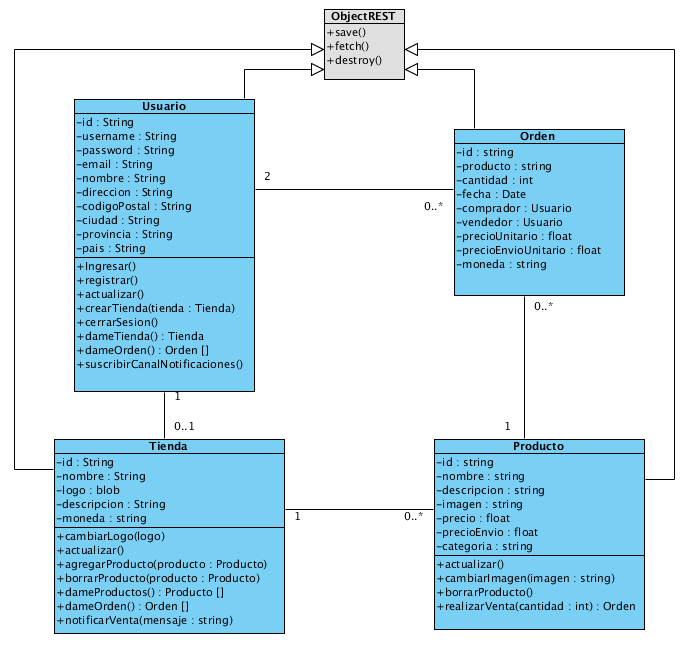
\includegraphics[width=1\textwidth]{imagenes/disenio/clases-disenio.png}
        %%Me parece que queda mejor sin el hfill
        %\hfill
    \label{fig:diagrama-clases-disenio}
\end{figure}

\section{Diagramas de Secuencia}

\subsection{Autenticar}
\begin{figure}[H]
  \centering
    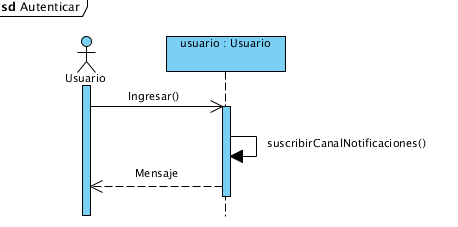
\includegraphics{imagenes/disenio/secuencia-autenticar.png}
        %%Me parece que queda mejor sin el hfill
        %\hfill
    \label{fig:diagrama-secuencia-autenticar}
\end{figure}


\subsection{Registrar}
\begin{figure}[H]
  \centering
    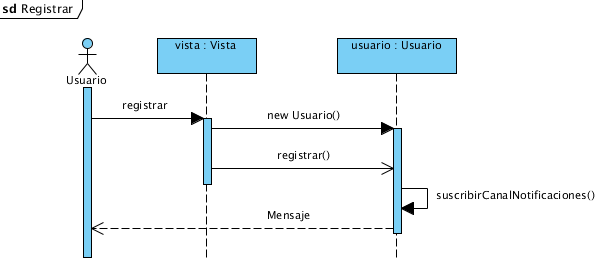
\includegraphics{imagenes/disenio/secuencia-registrar.png}
        %%Me parece que queda mejor sin el hfill
        %\hfill
    \label{fig:diagrama-secuencia-registrar}
\end{figure}

\subsection{Crear Tienda}
\begin{figure}[H]
  \centering
    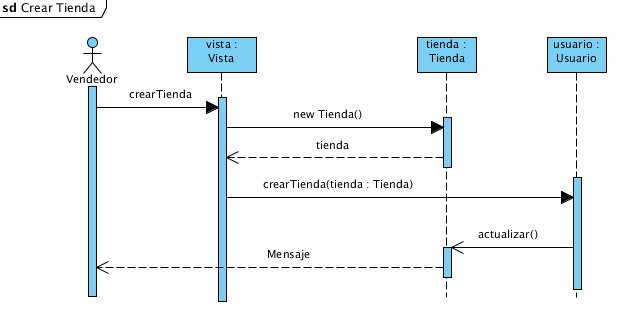
\includegraphics{imagenes/disenio/secuencia-crear-tienda.png}
        %%Me parece que queda mejor sin el hfill
        %\hfill
    \label{fig:diagrama-secuencia-crear-tienda}
\end{figure}

\subsection{Agregar Producto}
\begin{figure}[H]
  \centering
    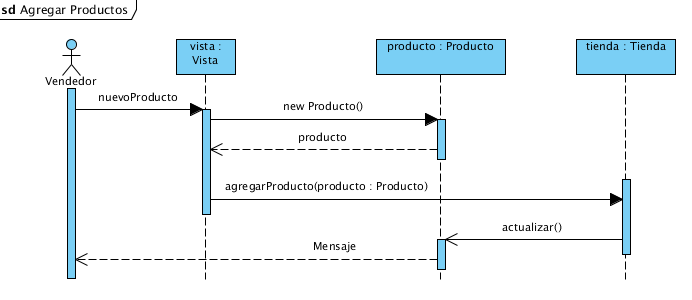
\includegraphics[width=1\textwidth]{imagenes/disenio/secuencia-agregar-producto.png}
        %%Me parece que queda mejor sin el hfill
        %\hfill
    \label{fig:diagrama-secuencia-agregar-producto}
\end{figure}

\subsection{Comprar Producto}
\begin{figure}[H]
  \centering
    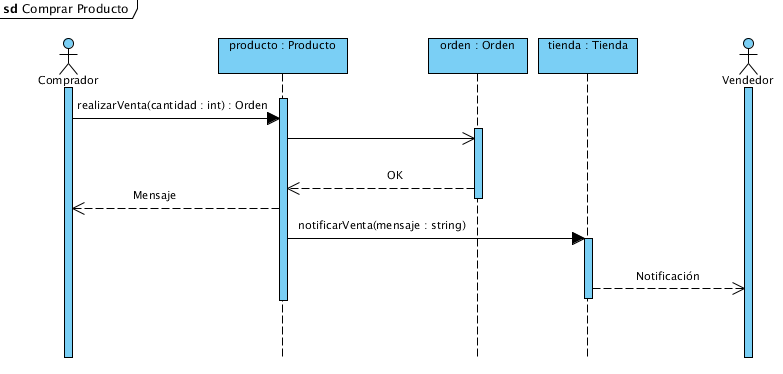
\includegraphics[width=1\textwidth]{imagenes/disenio/secuencia-comprar-producto.png}
        %%Me parece que queda mejor sin el hfill
        %\hfill
    \label{fig:diagrama-secuencia-comprar-producto}
\end{figure}

\section{Interfaz de Usuario}

\begin{figure}[H]
  \centering
    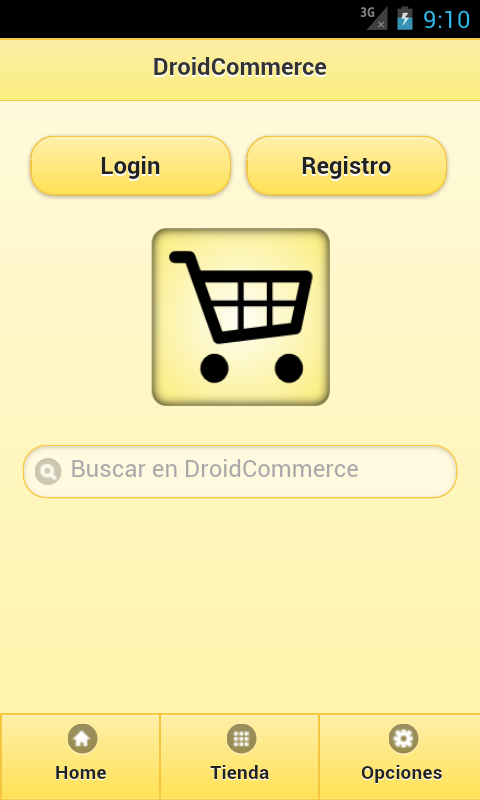
\includegraphics[width=0.6\textwidth]{imagenes/capturas/home.png}
        %%Me parece que queda mejor sin el hfill
        %\hfill
        \caption{Pantalla inicial}
    \label{fig:home}
\end{figure}

\begin{figure}
  \centering
    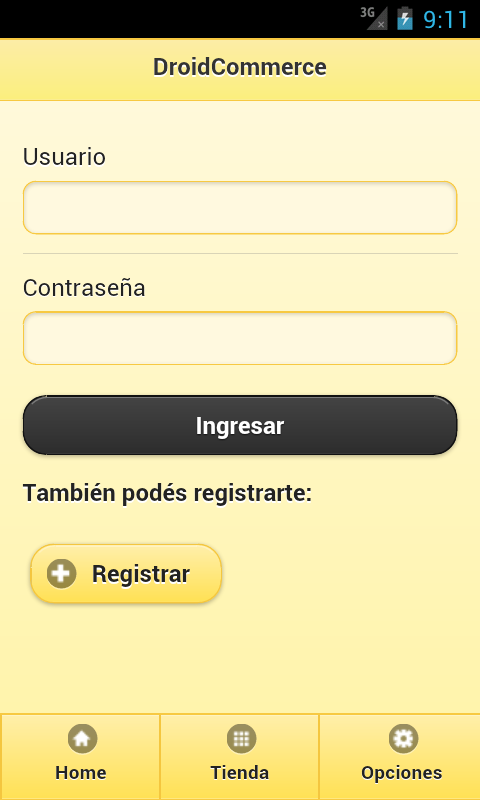
\includegraphics[width=0.6\textwidth]{imagenes/capturas/login.png}
        %%Me parece que queda mejor sin el hfill
        %\hfill
        \caption{Pantalla de login}
    \label{fig:login}
\end{figure}

\begin{figure}
  \centering
    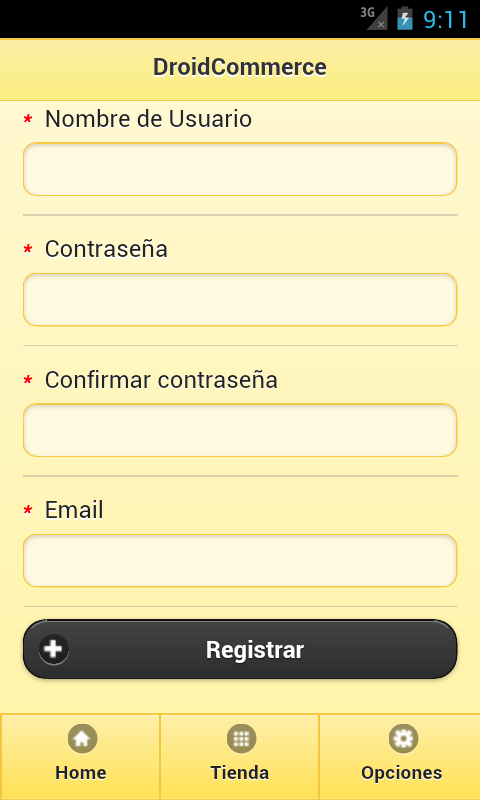
\includegraphics[width=0.6\textwidth]{imagenes/capturas/registro2.png}
        %%Me parece que queda mejor sin el hfill
        %\hfill
        \caption{Pantalla de registro}
    \label{fig:login}
\end{figure}

\begin{figure}
  \centering
    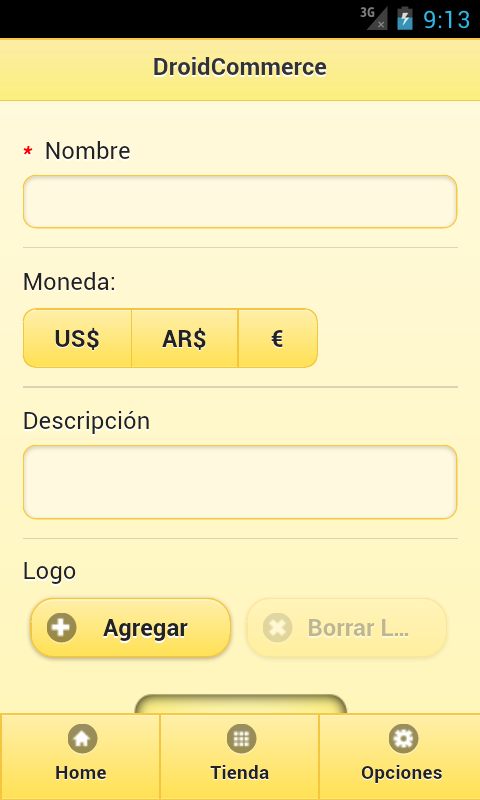
\includegraphics[width=0.6\textwidth]{imagenes/capturas/crear-tienda1.png}
        %%Me parece que queda mejor sin el hfill
        %\hfill
        \caption{Pantalla de creación de tienda, parte superior}
    \label{fig:crear-tienda-1}
\end{figure}

\begin{figure}
  \centering
    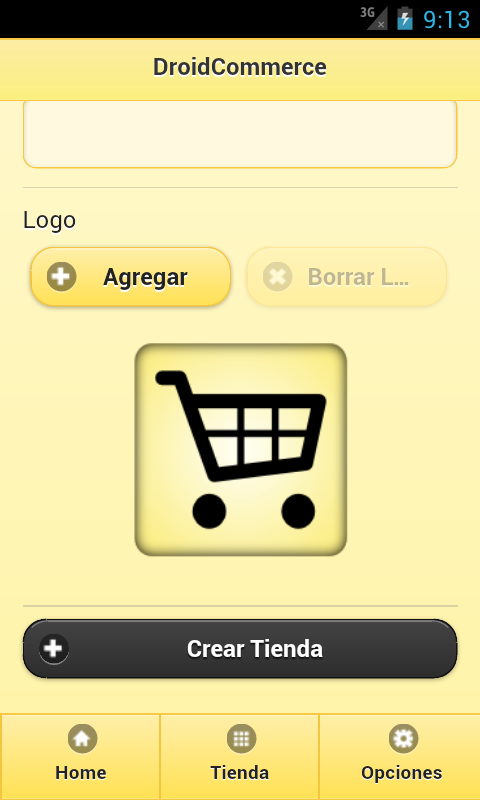
\includegraphics[width=0.6\textwidth]{imagenes/capturas/crear-tienda2.png}
        %%Me parece que queda mejor sin el hfill
        %\hfill
        \caption{Pantalla de creación de tienda, parte inferior}
    \label{fig:crear-tienda-2}
\end{figure}

\begin{figure}
  \centering
    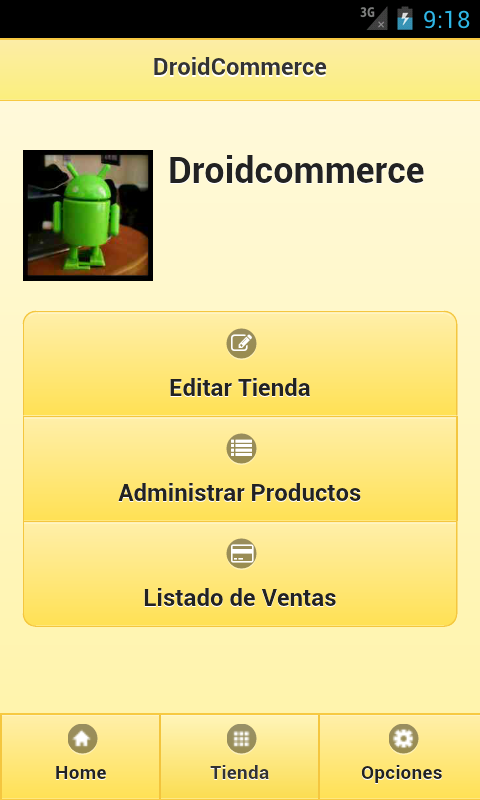
\includegraphics[width=0.6\textwidth]{imagenes/capturas/administracion-tienda.png}
        %%Me parece que queda mejor sin el hfill
        %\hfill
        \caption{Pantalla de administración de la tienda}
    \label{fig:admin-tienda}
\end{figure}


\begin{figure}
  \centering
    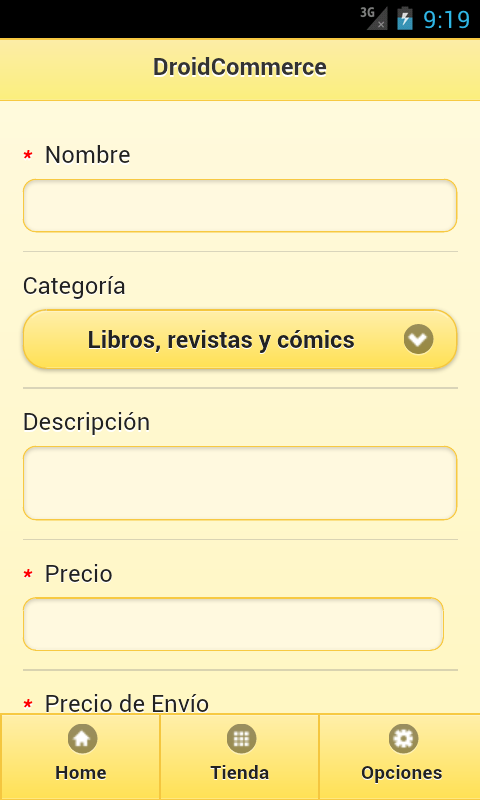
\includegraphics[width=0.6\textwidth]{imagenes/capturas/crear-producto1.png}
        %%Me parece que queda mejor sin el hfill
        %\hfill
        \caption{Pantalla de creación de producto, parte superior}
    \label{fig:crear-producto-1}
\end{figure}

\begin{figure}
  \centering
    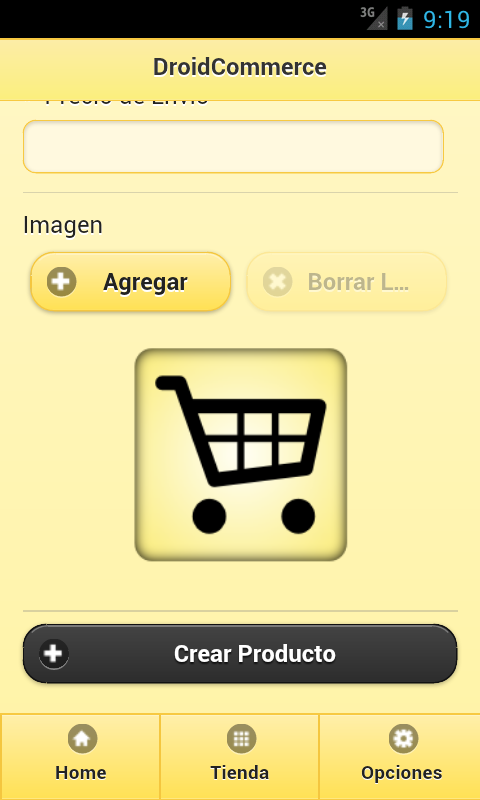
\includegraphics[width=0.6\textwidth]{imagenes/capturas/crear-producto2.png}
        %%Me parece que queda mejor sin el hfill
        %\hfill
        \caption{Pantalla de creación de producto, parte inferior}
    \label{fig:crear-producto2}
\end{figure}

\begin{figure}
  \centering
    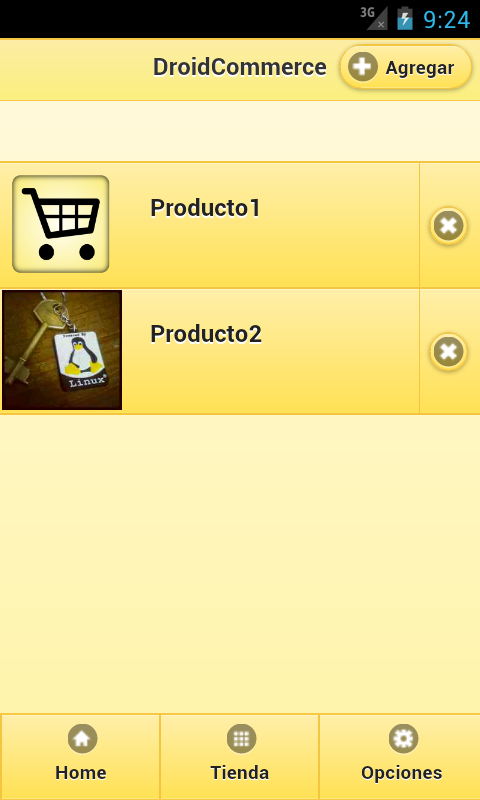
\includegraphics[width=0.6\textwidth]{imagenes/capturas/administracion-productos.png}
        %%Me parece que queda mejor sin el hfill
        %\hfill
        \caption{Pantalla de administración de productos}
    \label{fig:administrar-productos}
\end{figure}
\begin{figure}
  \centering
    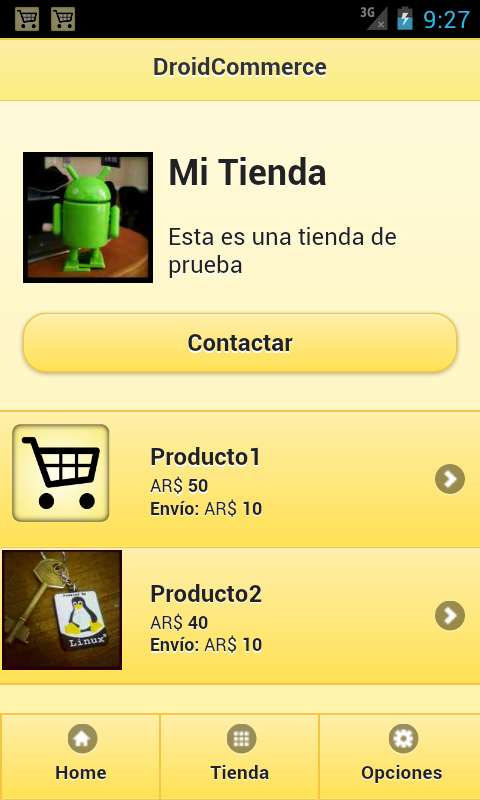
\includegraphics[width=0.6\textwidth]{imagenes/capturas/vista-tienda.png}
        %%Me parece que queda mejor sin el hfill
        %\hfill
        \caption{Pantalla de tienda}
    \label{fig:tienda}
\end{figure}

\begin{figure}
  \centering
    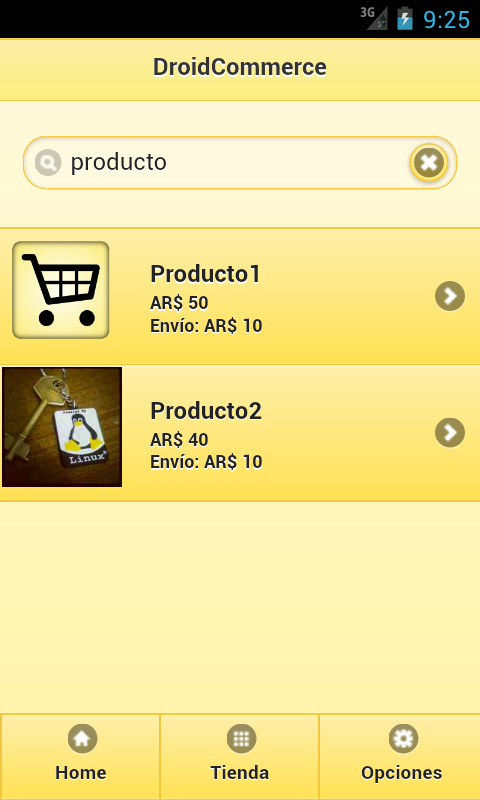
\includegraphics[width=0.6\textwidth]{imagenes/capturas/busqueda.png}
        %%Me parece que queda mejor sin el hfill
        %\hfill
        \caption{Pantalla de resultados de la búsqueda de productos}
    \label{fig:busqueda}
\end{figure}

\begin{figure}
  \centering
    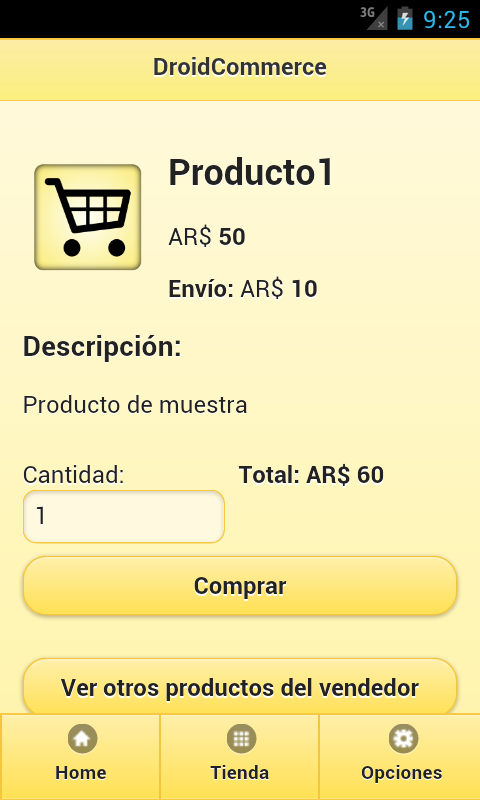
\includegraphics[width=0.6\textwidth]{imagenes/capturas/pagina-producto.png}
        %%Me parece que queda mejor sin el hfill
        %\hfill
        \caption{Pantalla de producto}
    \label{fig:producto}
\end{figure}

\begin{figure}
  \centering
    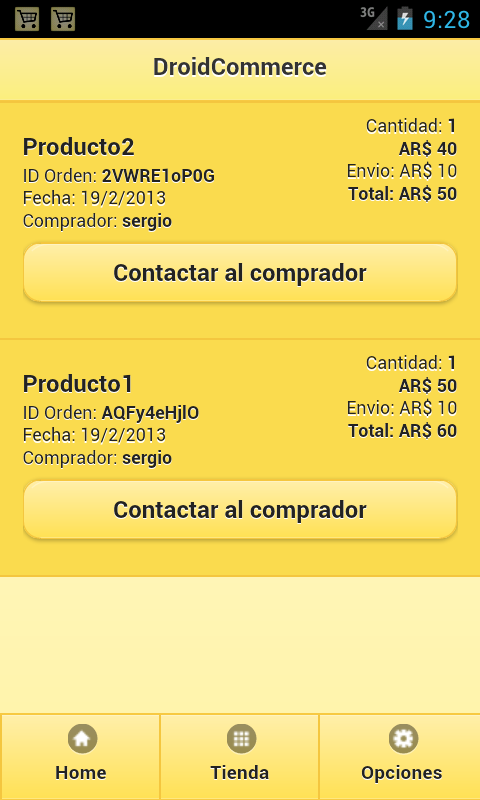
\includegraphics[width=0.6\textwidth]{imagenes/capturas/listado-ventas.png}
        %%Me parece que queda mejor sin el hfill
        %\hfill
        \caption{Pantalla de listado de ventas}
    \label{fig:listado-ventas}
\end{figure}

%% Disciplina de Implementación
%%%%%%%%%%%%%%%%%%%%%%%%%%%%%%%%%%%%%%%%%%%%%%%%%%%%%%%%
%   |------------------------------------------|       %
%   | Web App embebida en dispositivos móviles |       %
%   |  para la gestión de registros sobre la   |       %
%   |   contaminación de afluentes y ríos.     |       %
%   |                                          |       %
%   |          Proyecto de graduación          |       %
%   |__________________________________________|       %
%                                                      %
%   Autores                                            %
%   -------                                            %
%                                                      %
% * Bruno, Ricardo Hugo (CX 1409686)                   %
%     rburnount@gmail.com                              %
% * Gomez Veliz, Kevin Shionen (CX 1411828)            %
%     ing.gomezvelizkevin@gmail.com                    %
%                                                      %
%   Tutor                                              %
%   -------                                            %
%                                                      %
% * Ing. Cohen, Daniel Eduardo                         %
%        dcohen.tuc@gmail.com                          %
%                                                      %
%   Cotutor                                            %
%   -------                                            %
%                                                      %
% * Ing. Nieto, Luis Eduardo                           %
%        lnieto@herrera.unt.edu.ar                     %
%                                                      %
%                                                      %
%%%%%%%%%%%%%%%%%%%%%%%%%%%%%%%%%%%%%%%%%%%%%%%%%%%%%%%%

\chapter{Disciplina de Implementación}
\label{chap:implementacion}

\section{Diagrama conceptual estructura Cliente/Servidor/Internet}
    \begin{figure}[H]
        \centering
        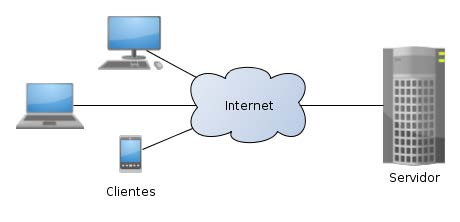
\includegraphics[width=1\textwidth]{imagenes/implementacion/clienteServidorInternet.jpg}
        \label{clienteServidorInternet}
    \end{figure}


\section{Arquitectura de la aplicación}

\begin{figure}[H]
  \centering
    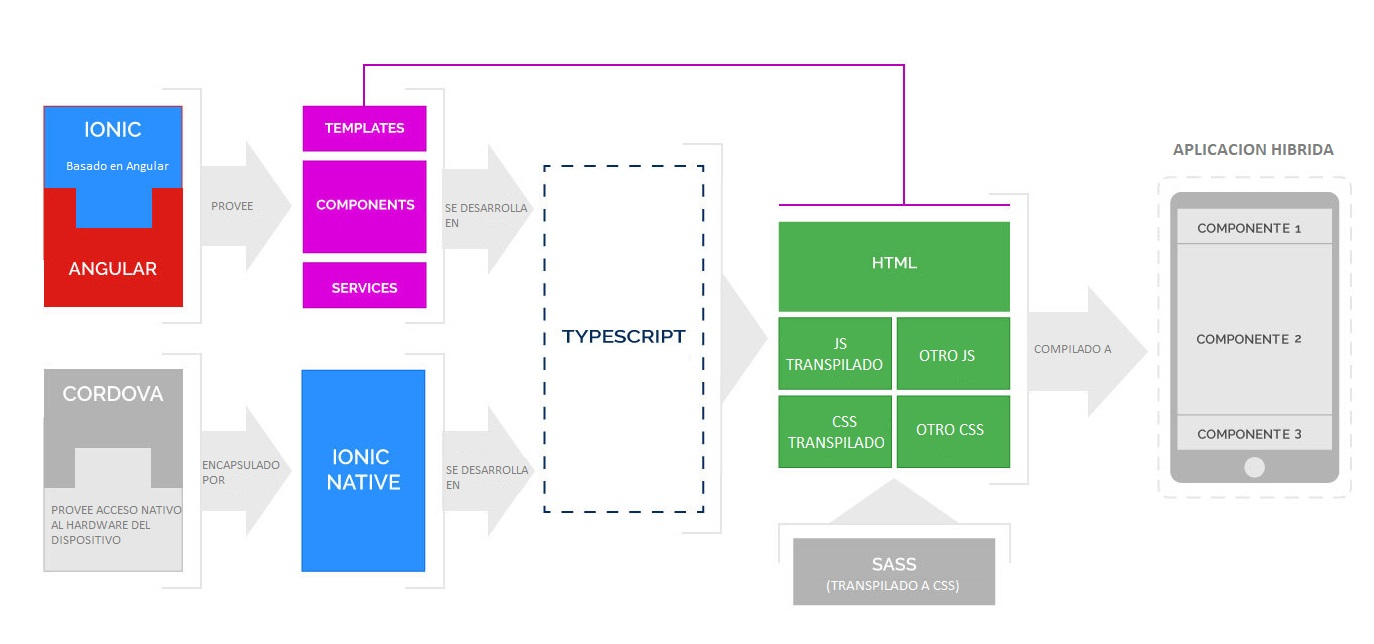
\includegraphics[width=1\textwidth]{imagenes/implementacion/interfazDeUsuario.jpg}
    
     \caption{Interfaz de Usuario}
    \label{fig:arquitectura-aplicacion}
\end{figure}

    \begin{figure}[H]
        \centering
        %lo que agregué entre corchetes hace que el ancho de la imagen ocupe el 80% del área de texto. Si sacás eso la imagen no se redimensiona y se va de la hoja. Se puede usar algo parecido para limitar el alto si es necesario.
        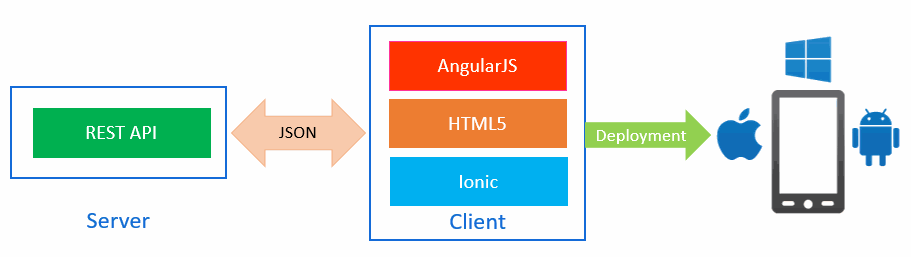
\includegraphics[width=1\textwidth]{imagenes/implementacion/despliegue.png}
        \caption{Diagrama de Despliegue}
        \label{diagrama-despliegue}
    \end{figure}


\section{Modelo-Vista-Controlador}

Modelo-Vista-Controlador (en adelante MVC) es un patron de diseño que permite
separar la capa de datos y logica de negocios (modelos y controladores), de la interfaz
de usuario (vista).

\subsection{Componentes del patrón}
\begin{itemize}
    \item \textbf{Modelo}: Es la representacion de la informacion con la cual el sistema opera. Se
    puede pensar en un modelo como una tabla en el sistema gestor de bases de datos.
    Si bien este enfoque resulta sumamente util para trabajar con el patron MVC,
    el modelo tambien requiere de funcionalidades que faciliten la interaccion con los
    demas controladores, vistas y modelos del sistema.
    \item \textbf{Vista}: Es la representacion grafica de los datos. Provee la interfaz mediante la cual
    los usuarios realizan la entrada de los datos y observan el resultado del procesamiento
    de dichos datos.
    \item \textbf{Controlador}: Sirve como nexo entre las vistas y los modelos. El controlador responde
    usualmente a eventos que son generados por el usuario en su interaccion con
    la vista. La vista brinda al usuario un mecanismo para comunicarse con un controlador,
    y es este ultimo el encargado de obtener los datos ingresados por el usuario,
    pasarlos al modelo adecuado para su procesamiento, recibir la salida del modelo y
    enviar dicha salida a la vista para su visualizacion.
    
\end{itemize}



\section{Elección del Lenguaje}

    Independientemente del paradigma de ingeniería de software, el lenguaje de programación tendrá impacto en la planificación, el análisis, el diseño, la codificación, la prueba y el mantenimiento de un proyecto. Para la construcción de la aplicación se eligió la utilización de los lenguajes web HTML5, CSS3 y JavaScript.

    La elección de estos lenguajes para la construcción de la apliación se debe a las siguientes ventajas que ofrecen:
    \begin{itemize}
        \item \emph{Mayor portabilidad:} Al ser tecnologías estándares y soportadas por la mayoría de los teléfonos celulares modernos, es posible que una misma aplicación sea muy fácilmente adaptable a varias plataformas móviles.
        \item \emph{Soporte futuro:} Todas las plataformas móviles están trabajando para mejorar el soporte que ofrecen a las tecnologías web, ofreciendo una mejor experiencia al usuario.
        \item \emph{Aprovechamiento de conocimiento de desarrollo de aplicaciones web:} Desarrollando aplicaciones móviles en \gls{HTML}5, \gls{CSS}3 y \gls{JavaScript} es posible aplicar el conocimiento en el desarrollo de aplicaciones web desarrolladas para navegadores en equipos de escritorio 
    \end{itemize}

\section{Apache Cordova}

\begin{figure}[H]
  \centering
    %lo que agregué entre corchetes hace que el ancho de la imagen ocupe el 80% del área de texto. Si sacás eso la imagen no se redimensiona y se va de la hoja. Se puede usar algo parecido para limitar el alto si es necesario.
    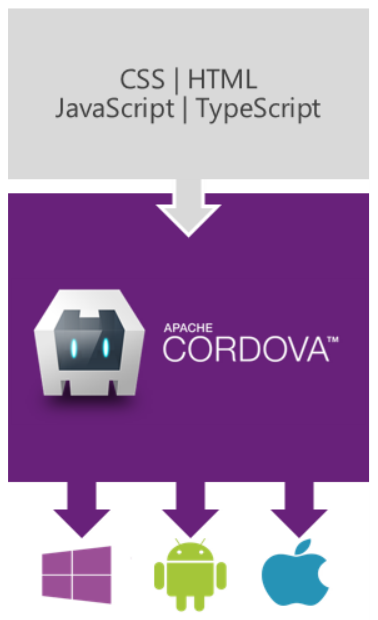
\includegraphics[width=0.5\textwidth]{imagenes/cordova-architecture.png}
    
     \caption{Arquitectura de Apache Cordova}
    \label{arquitectura-Apache Cordova}
\end{figure}

Apache Cordova es un \gls{framework} de código abierto que actúa como un intermediario entre las aplicaciones web y los dispositivos móviles. Permite crear aplicaciones móviles instalables utilizando tecnología web: \gls{JavaScript}, \gls{HTML}5 y \gls{CSS}3.

Las aplicaciones resultantes no son totalmente nativas, ni puramente basado en la web. La desventaja de que una aplicación sea totalmente nativa es que sólo se podrá utilizar para la plataforma para la que fue realizada, es decir si se hace una aplicación para Android luego no se podrá reutilizar el código para hacer la misma aplicación para iOS.

Con Apache Cordova se puede reutilizar el código de una aplicación para crear el paquete instalable de cualquiera de las 7 plataformas móviles soportadas: iOS, Android, Blackberry, Windows Phone, WebOS de Palm, Symbianm, Bada, entre otras.

Apache Cordova permite acceder a funciones nativas como el acelerómetro, cámara, brújula, contactos, archivos, ubicación geográfica, almacenamiento  y notificaciones.

\subsection{Ventajas de Apache Cordova}

\begin{itemize}

    \item Soporte multiplataforma
    
    \item Acceso a características nativas de cada plataforma a través de su API, a las que una aplicación web visitada desde el navegador no podría acceder, como acceso a la cámara de fotos, acelerómetro, notificaciones, etc.
    
    \item Permite ejecutar a través de JavaScript plugins escritos en código nativo.
    
    \item Permite distribuir aplicaciones realizadas utilizando HTML5 y JavaScript a través de las tiendas de aplicaciones oficiales de cada plataforma.
    
    \end{itemize}
    \subsection{Desventaja de Apache Cordova}
    \begin{itemize}
\item Normalmente las aplicaciones realizadas con Apache Cordova tienen un menor rendimiento en tareas que requieren alta capacidad de procesamiento, sobre todo en versiones antiguas de las plataformas sobre las que se usa.

\item Se pierde la posibilidad de acceder a algunas características nativas, como los diferentes elementos de interfaz de usuario propios de cada plataforma, aunque estos pueden imitarse mediante el uso de CSS.
\end{itemize}

\section{Web services}
\label{sec:webservices}

Un servicio web (en inglés, Web service) es una tecnología que utiliza un conjunto de protocolos y estándares que sirven para intercambiar datos entre aplicaciones. Distintas aplicaciones de software desarrolladas en lenguajes de programación diferentes, y ejecutadas sobre cualquier plataforma, pueden utilizar los servicios web para intercambiar datos en redes de ordenadores como Internet. La interoperabilidad se consigue mediante la adopción de estándares abiertos.

Las ventajas de los servicios web son:

\begin{itemize}
    \item Aportan interoperabilidad entre aplicaciones de software independientemente de sus propiedades o de las plataformas sobre las que se instalen.
    \item Los servicios Web fomentan los estándares y protocolos basados en texto, que hacen más fácil acceder a su contenido y entender su funcionamiento.
    \item Permiten que servicios y software de diferentes compañías ubicadas en diferentes lugares geográficos puedan ser combinados fácilmente para proveer servicios integrados.
   
 \end{itemize}
 
\subsection{Razones para crear servicios Web}

La principal razón para usar servicios Web es que se pueden utilizar con HTTPS sobre \gls{TCP} en el puerto 443. Dado que las organizaciones protegen sus redes mediante firewalls -que filtran y bloquean gran parte del tráfico de Internet, cierran casi todos los puertos TCP salvo el 443, que es, precisamente, el que usan los navegadores. Los servicios Web utilizan este puerto, por la simple razón de que no resultan bloqueados. Es importante señalar que los servicios web se pueden utilizar sobre cualquier protocolo, sin embargo, TCP es el más común.

Otra razón por la que los servicios Web son muy prácticos es que pueden aportar gran independencia entre la aplicación que usa el servicio Web y el propio servicio. De esta forma, los cambios a lo largo del tiempo en uno no deben afectar al otro. Esta flexibilidad será cada vez más importante, dado que la tendencia a construir grandes aplicaciones a partir de componentes distribuidos más pequeños es cada día más utilizada.
Se pueden desarrollar servicios web como parte de una aplicación web, permitiendo acceder a los mismos datos que esta.


\subsection{REST}

REST es una técnica de arquitectura software para sistemas hipermedia distribuidos como la World Wide Web.
Los sistemas que siguen los principios REST se llaman con frecuencia RESTful.

\begin{figure}[htbp]
  \centering
    %lo que agregué entre corchetes hace que el ancho de la imagen ocupe el 80% del área de texto. Si sacás eso la imagen no se redimensiona y se va de la hoja. Se puede usar algo parecido para limitar el alto si es necesario.
    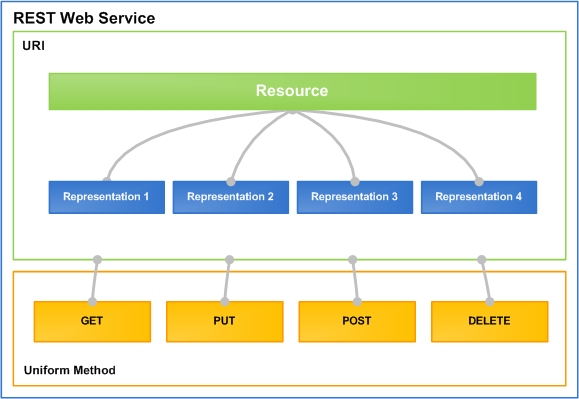
\includegraphics[width=0.8\textwidth]{imagenes/REST.jpg}
    
     \caption{Web Services REST}
    \label{fig:REST}
\end{figure}

REST afirma que la web ha disfrutado de escalabilidad como resultado de una serie de diseños fundamentales clave:

\begin{itemize}
    \item \emph{Un protocolo cliente/servidor sin estado:} cada mensaje HTTP contiene toda la información necesaria para comprender la petición. Como resultado, ni el cliente ni el servidor necesitan recordar ningún estado de las comunicaciones entre mensajes. Sin embargo, en la práctica, muchas aplicaciones basadas en HTTP utilizan cookies y otros mecanismos para mantener el estado de la sesión (algunas de estas prácticas, como la reescritura de URLs, no son permitidas por REST)
    
    \item \emph{Un conjunto de operaciones bien definidas que se aplican a todos los recursos de información:} HTTP en sí define un conjunto pequeño de operaciones, las más importantes son POST, GET, PUT y DELETE.
    
    \item Una sintaxis universal para identificar los recursos. En un sistema REST, cada recurso es direccionable únicamente a través de su \gls{URI}.
   
 \end{itemize}
 
 \subsubsection{Recursos}
 Un concepto importante en REST es la existencia de recursos (elementos de información), que pueden ser accedidos utilizando un identificador global (un Identificador Uniforme de Recurso).
 
 Para manipular estos recursos, los componentes de la red (clientes y servidores) se comunican a través de una interfaz estándar (HTTP) e intercambian representaciones de estos recursos (los ficheros que se descargan y se envían.
 
\section{Express.js}

Express es una infraestructura de aplicaciones web Node.js mínima y flexible que proporciona un conjunto sólido de características para las aplicaciones web y móviles.
Con miles de métodos de programa de utilidad HTTP y middleware a su disposición, la creación de una API sólida es rápida y sencilla.
Express proporciona una delgada capa de características de aplicación web básicas, que no ocultan las características de Node.js.

\section{Herramientas de desarrollo}

\begin{itemize}

\item \emph {Visual Code:} Visual Studio Code es un editor de código fuente desarrollado por Microsoft para Windows , Linux y macOS. Incluye soporte para la depuración, control integrado de Git.Es gratuito y de código abierto.

\item \emph {Draw.io:} Es un stack de tecnología de codigo abierto para crear aplicaciones de diagramación, entre ellas UML.
Permite dibujar todos los tipos de diagramas de clases, código inverso, generar código desde diagramas y generar documentación.

\item \emph{\LaTeX:} Es un sistema de composición de textos, orientado especialmente a la creación de libros, documentos científicos y técnicos que contengan fórmulas matemáticas.

\LaTeX facilita el uso del lenguaje de composición tipográfica. Es muy utilizado para la composición de artículos académicos, tesis y libros técnicos, dado que la calidad tipográfica de los documentos realizados con \LaTeX es comparable a la de una editorial científica de primera línea.

\item \emph{GitHub:} Es una forja (plataforma de desarrollo colaborativo) para alojar proyectos utilizando el sistema de control de versiones Git. Se utiliza principalmente para la creación de código fuente de programas de computadora.

\end{itemize}



%% Disciplina de Pruebas
%%%%%%%%%%%%%%%%%%%%%%%%%%%%%%%%%%%%%%%%%%%%%%%%%%%%%%%%
%   |------------------------------------------|       %
%   | Web App embebida en dispositivos móviles |       %
%   |  para la gestión de registros sobre la   |       %
%   |   contaminación de afluentes y ríos.     |       %
%   |                                          |       %
%   |          Proyecto de graduación          |       %
%   |__________________________________________|       %
%                                                      %
%   Autores                                            %
%   -------                                            %
%                                                      %
% * Bruno, Ricardo Hugo (CX 1409686)                   %
%     rburnount@gmail.com                              %
% * Gómez Veliz, Kevin Shionen (CX 1411828)            %
%     ing.gomezvelizkevin@gmail.com                    %
%                                                      %
%   Tutor                                              %
%   -------                                            %
%                                                      %
% * Ing. Cohen, Daniel Eduardo                         %
%        dcohen.tuc@gmail.com                          %
%                                                      %
%   Cotutor                                            %
%   -------                                            %
%                                                      %
% * Ing. Nieto, Luis Eduardo                           %
%        lnieto@herrera.unt.edu.ar                     %
%                                                      %
%                                                      %
%%%%%%%%%%%%%%%%%%%%%%%%%%%%%%%%%%%%%%%%%%%%%%%%%%%%%%%%

\chapter{Disciplina de Pruebas}
\label{chap:pruebas}

\section{Test de Unidades}
	\subsection{Introducción}

		El Test de Unidades consiste en realizar pruebas de las unidades individuales de código. En esta fase se realizan las pruebas de caja blanca. 

	\subsection{Pruebas de Caja Blanca}
		Es un tipo de método de prueba que permite detectar errores internos del código de cada módulo. 

		Con estas pruebas se pueden garantizar que se ejercitan por lo menos una vez todos los caminos independientes de cada módulo, que las decisiones lógicas se evalúan en sus dos variantes (verdadera y falsa), que se ejecutan todos los bucles en sus límites operacionales y que se ejercitan las estructuras internas de datos para asegurar su validez.
		\newline

		\textbf{Pruebas realizadas:}
		Para el mantenimiento del código, se implementaron test unitarios por módulos, para asegurarse que el código este siempre funcionando correctamente. Algunos de los módulos con test unitarios son: formulario para alta usuario, formulario para nuevos registros, entre otros.
		Todos estos test son usados para controlar la integridad de los datos ingresados.

\section{Test de Módulos}

	\subsection{Introducción}
		El Test de Módulos consiste en realizar pruebas de los módulos funcionales del sistema. En esta fase se realizan las pruebas de caja negra y las pruebas de estrés. 

	\subsection{Pruebas de Caja Negra}

		En este método de prueba se ve a cada módulo como una caja negra y se generan conjuntos de condiciones de entrada que ejerciten completamente todos los requisitos funcionales del programa, observando las salidas.

		Con estas pruebas se pueden detectar funciones incorrectas o ausentes, errores de interfaz, errores de rendimiento, etc.
		\newline

		\textbf{Pruebas realizadas:}
		Al finalizar los módulos, se realizaron los test de caja negra correspondientes, validando así que la entradas de datos genere la salida esperada.
		Por ejemplo, al crear un registro, si no se capturo la foto de la muestra, el usuario recibe el correspondiente mensaje de error. Esta acción se realiza para los requisitos obligatorios de un registro, hasta comprobar su validez, para luego ser guardado en la base de dato.
			
	\subsection{Pruebas de Estrés}

		Esta prueba se centra en realizar el análisis de valores límites, y en condiciones límites, ya que se ha demostrado que los errores tienden a darse más en los límites del campo de entrada y sometidos a condiciones límites.

		\newpage
		\textbf{Pruebas realizadas:}
		Para las pruebas de estrés se sometió a la base de datos no relacional (couchDB) a la creación de 100 registros prototipo, donde obtuvieron los siguientes resultados no satisfactorios:
		\begin{itemize}
			\item Demora en la sincronización entre las BD.
			\item Falla en la sincronización.
			\item La BD crecía exponencialmente su tamaño debido al versionado nativo de los documentos al actualizarlos.
		\end{itemize}
		Por estos motivos, se rediseño el sistema para trabajar con una BD Relacional (MySql) realizando los siguientes cambios:
		\begin{itemize}
			\item Se modifico el protocolo de comunicación entre el sistema y el servidor
			\item Se creo un protocolo de sincronización automática que se ajusta a los requisitos del sistema
			\item Se implemento web socket para ver los cambios de la sincronización en tiempo real.
		\end{itemize}
		
		\textbf{Pruebas realizadas con el rediseño:}

		Se realizaron las mismas pruebas, pero esta vez, con resultados satisfactorios para todos los punto enunciados anteriormente.


\section{Test de Integración}

	\subsection{Introducción}

		El Test de Integración consiste en realizar pruebas de la estructura modular del programa y su interacción a través de la prueba de integración.

	\subsection{Pruebas de Integración}

		En este tipo de prueba los errores surgen al integrar los módulos. En esta fase se pueden detectar errores como por ejemplo que las subfunción, es cuando se combinan pueden no producir la función principal, un módulo puede tener un efecto adverso e inadvertido sobre otro, etc.

		El objetivo es tomar los módulos probados y construir una estructura de programa que esté de acuerdo con lo que dicta la especificación C.
			
		Existen dos tipos de integración:
			\begin{itemize}
				\item \textbf{Integración descendente:} En este tipo se integran los módulos moviéndose hacia abajo por la jerarquía de control, comenzando con el módulo de control inicial.
				\item \textbf{Integración ascendente:} En este tipo se integran los módulos atómicos primero y luego se continúa con el nivel inmediato superior.
			\end{itemize}

	En el desarrollo de este sistema se utilizó la integración descendente. Probando a mano, todos los casos escenarios posibles, como por ejemplo:
	\begin{itemize}
		\item Creación de registros.
		\item Iniciar sesión
		\item Comprobar el estado del mapa general, con los registros validados.
		\item Acceder al perfil
	\end{itemize}
	Todos estos casos fueron probados de manera online y offline.
	En funciones como ver el mapa general, que requieren conexión a internet y nos encontramos offline, se muestra un mensaje de alerta y no se permite el acceso a dicha función. Por otro lado, funciones que no requieren conexión a internet, de manera offline, pueden ser accedidas sin problemas

\section{Test de Aceptación}

	\subsection{Introducción}

		El Test de Aceptación consiste en realizar la prueba del software para validar si funciona de acuerdo con las expectativas razonables del cliente. En esta fase se llevan a cabo las pruebas Alfa y Beta.

	\subsection{Prueba Alfa}

		Esta prueba es conducida por el cliente en el lugar de desarrollo. Se usa el software de forma natural (previa capacitación), con el encargado de desarrollo mirando “por encima del hombro” del usuario y registrando errores y problemas de uso. Se lleva acabo en un entorno controlado.

		\textbf{Conclusiones de estas pruebas:}
		Tras esta prueba, nos dimos cuenta de algunos errores y posibles mejoras, no solo de funcionamiento, sino también de la interfaz de usuario, ya que no era muy amigable. 
		Para estas prueba se realizo una salida de campo real con el cliente (docente Daniel Dos Santos), en las cuales pudimos apreciar si nuestro sistema se adecuo correctamente a los requisitos planteados.
		Estas pruebas se realizaron con un smartphone de gama baja, asegurando que, siendo el peor de los casos, se obtuvieron fotos legibles, coordenadas del GPS correctas, fluidez en la interfaz de usuario y un buen \textit{performance} del dispositivo móvil en lo se refiere a procesamiento.
		\newpage 

		\textbf{Fotos de la salida de campo:}

		\begin{figure}[H]
			\centering
				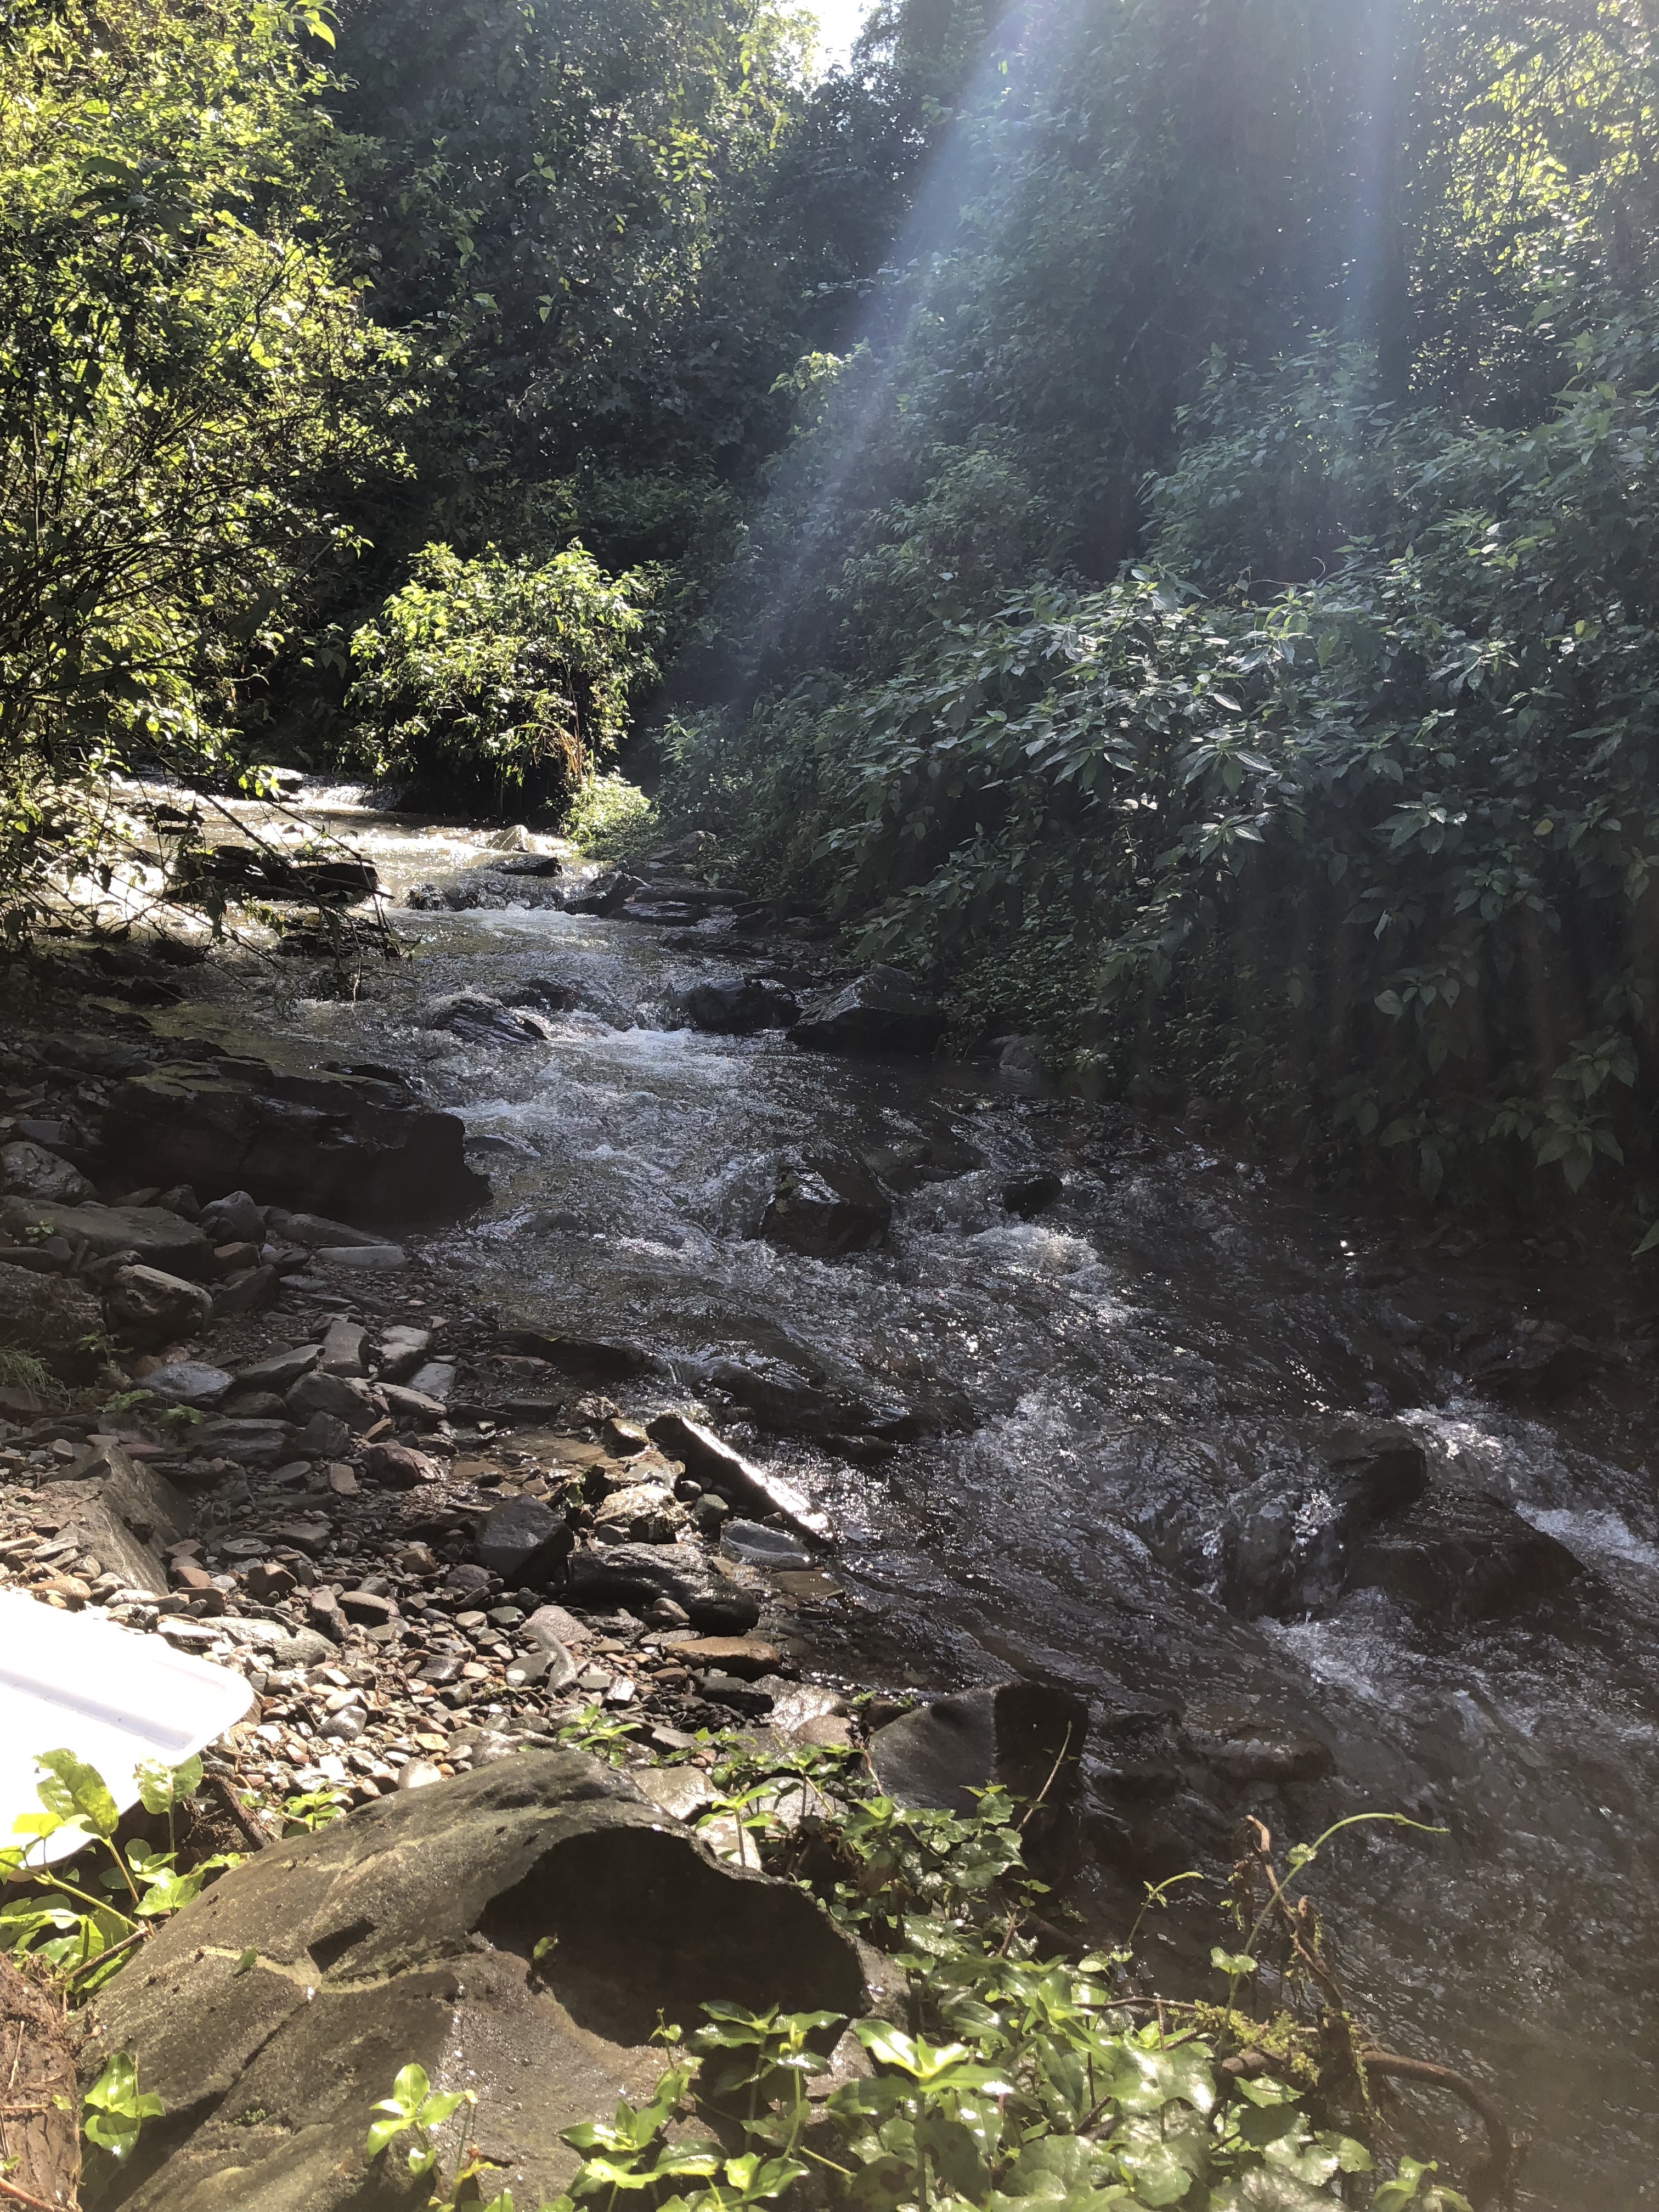
\includegraphics[width=1\textwidth]{imagenes/testAlpha/1.JPG}
					\caption{Foto paisaje de la muestra que sirve para futuro reconocimiento}
		\end{figure}
		\begin{figure}[H]
			\centering
				\includegraphics[width=1\textwidth]{imagenes/testAlpha/2.JPG}
					\caption{Red de pie utilizada para la obtención de la muestra}
		\end{figure}
		\begin{figure}[H]
			\centering
				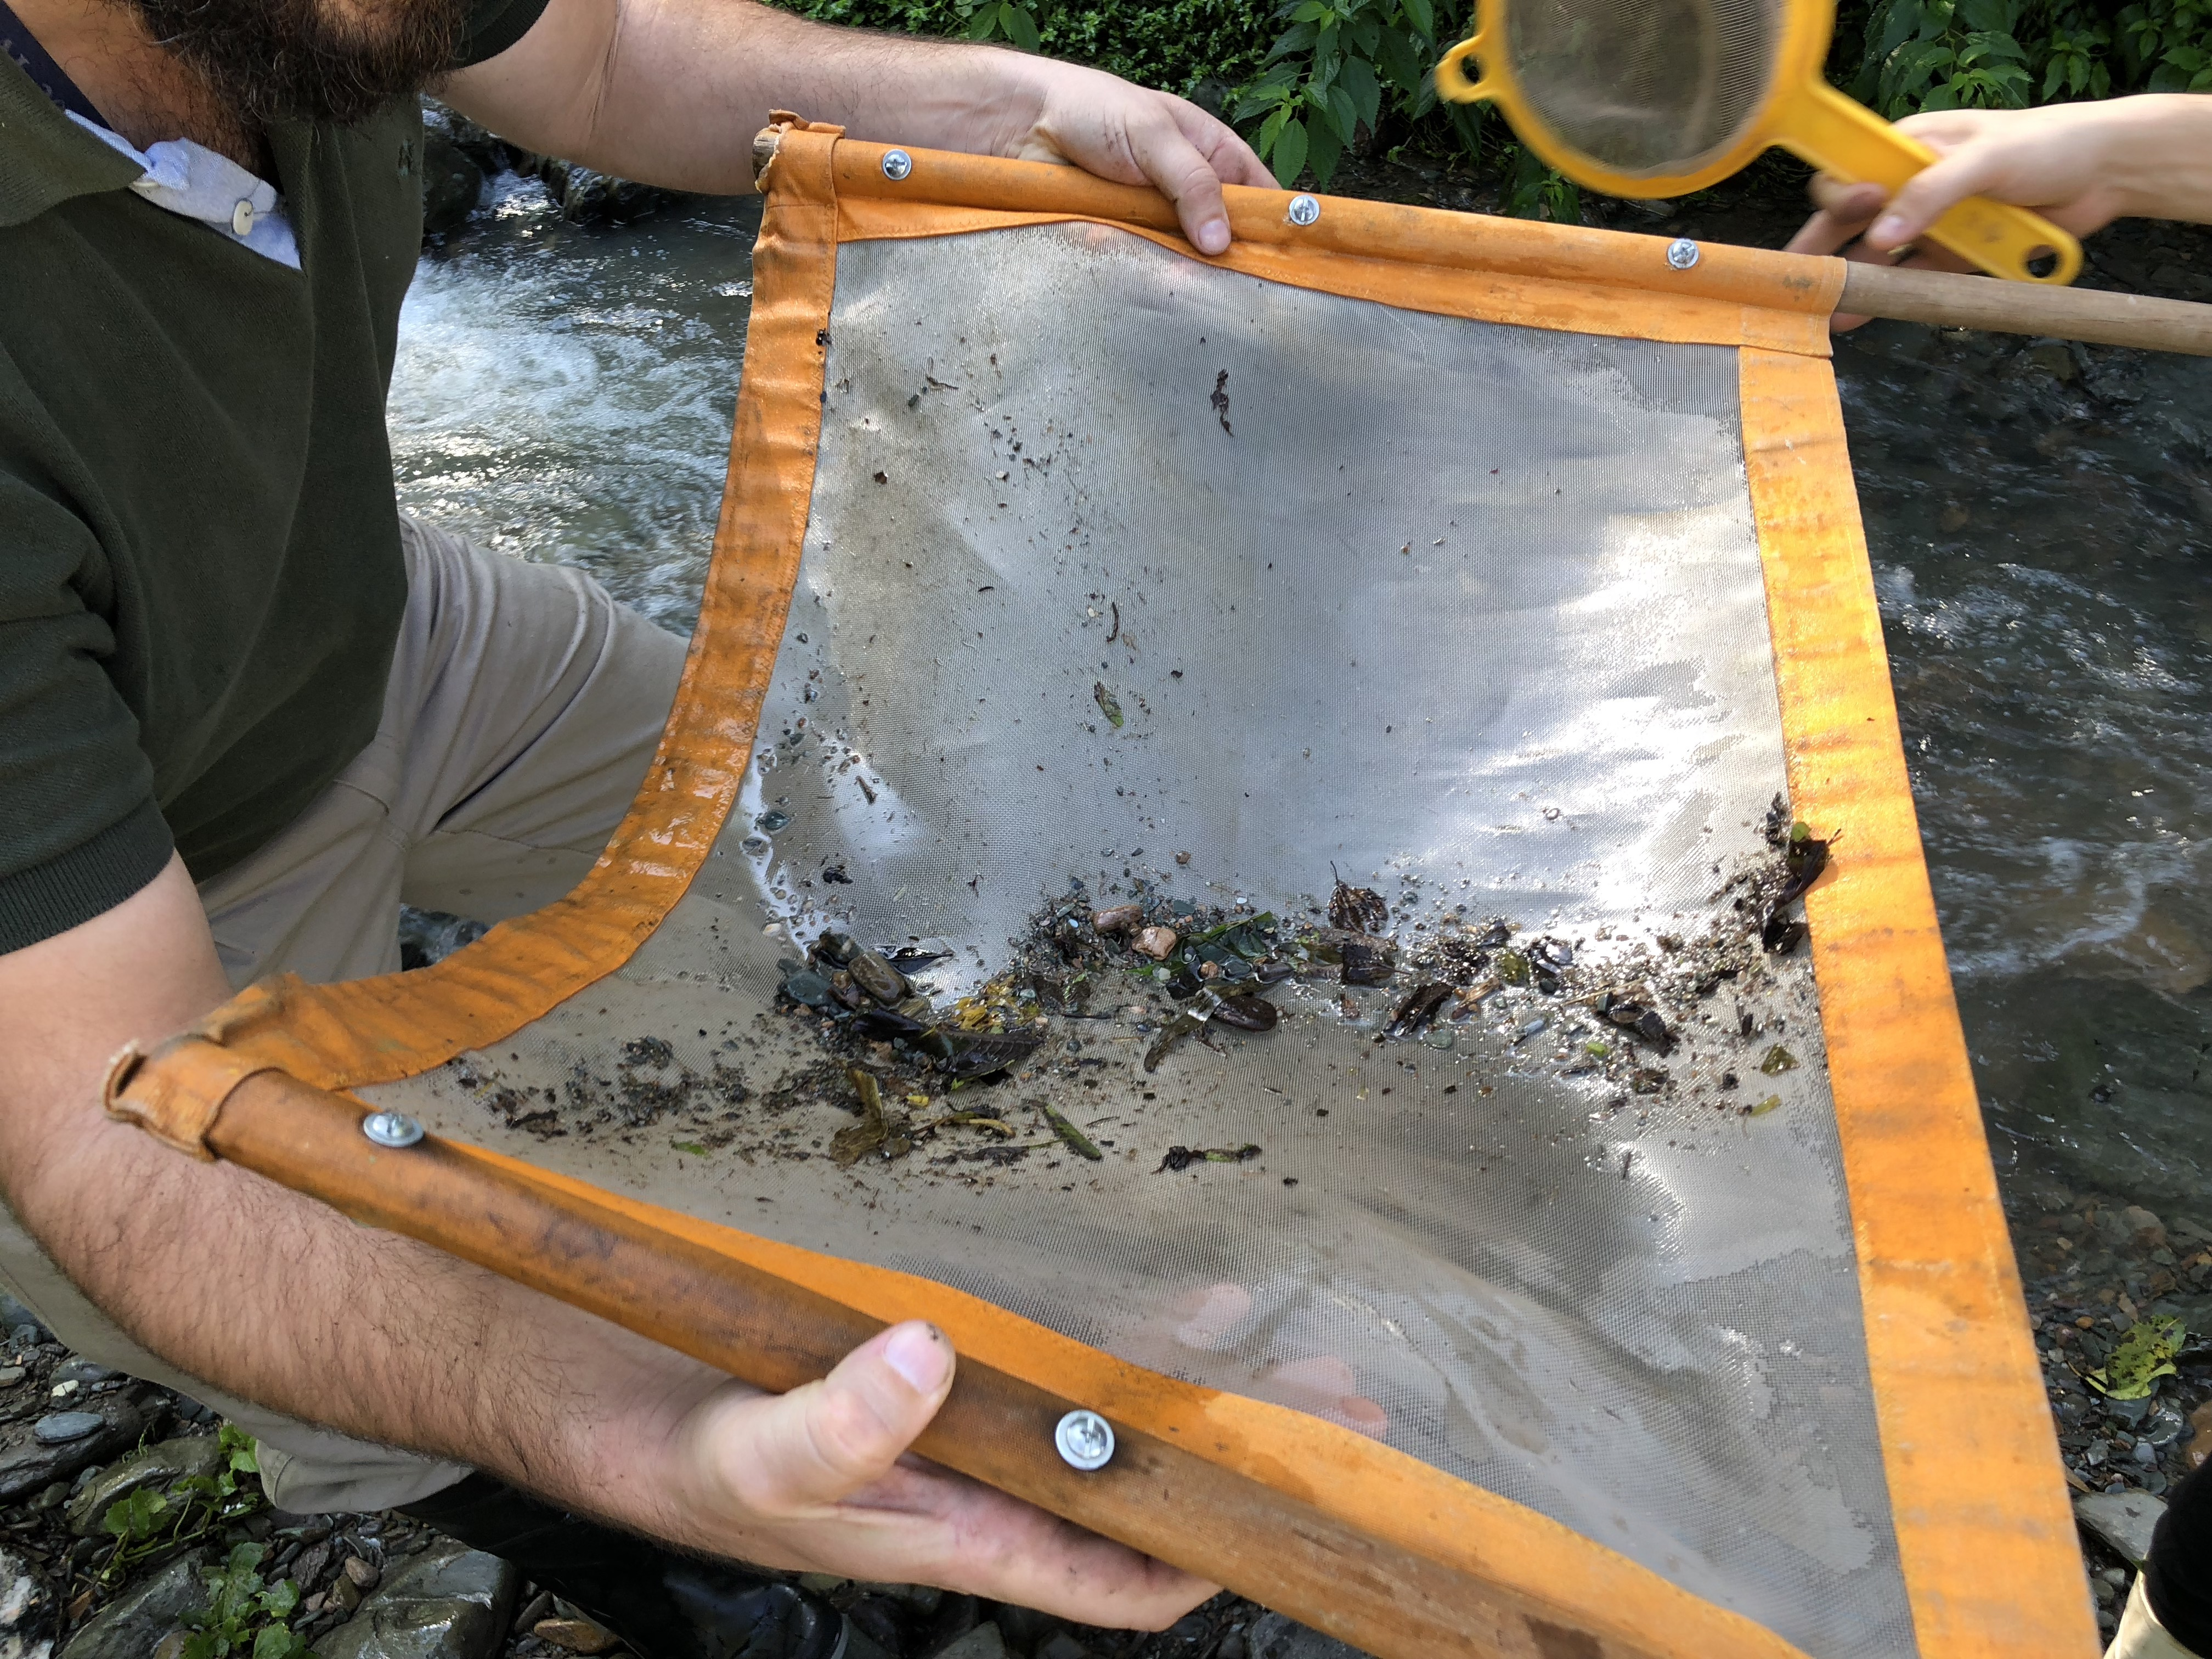
\includegraphics[width=1\textwidth]{imagenes/testAlpha/3.JPG}
					\caption{Proceso de validación de la muestra}
		\end{figure}
		\begin{figure}[H]
			\centering
				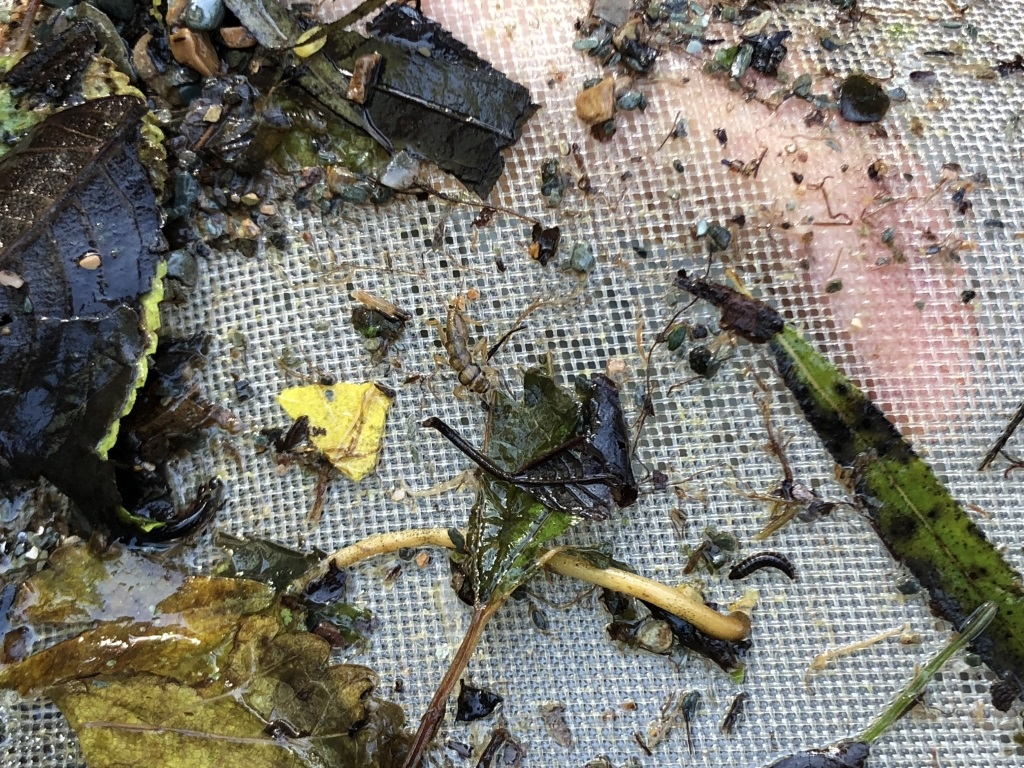
\includegraphics[width=1\textwidth]{imagenes/testAlpha/4.JPG}
					\caption{Proceso de identificación y extracción de los insectos objetivos}
		\end{figure}
		\begin{figure}[H]
			\centering
				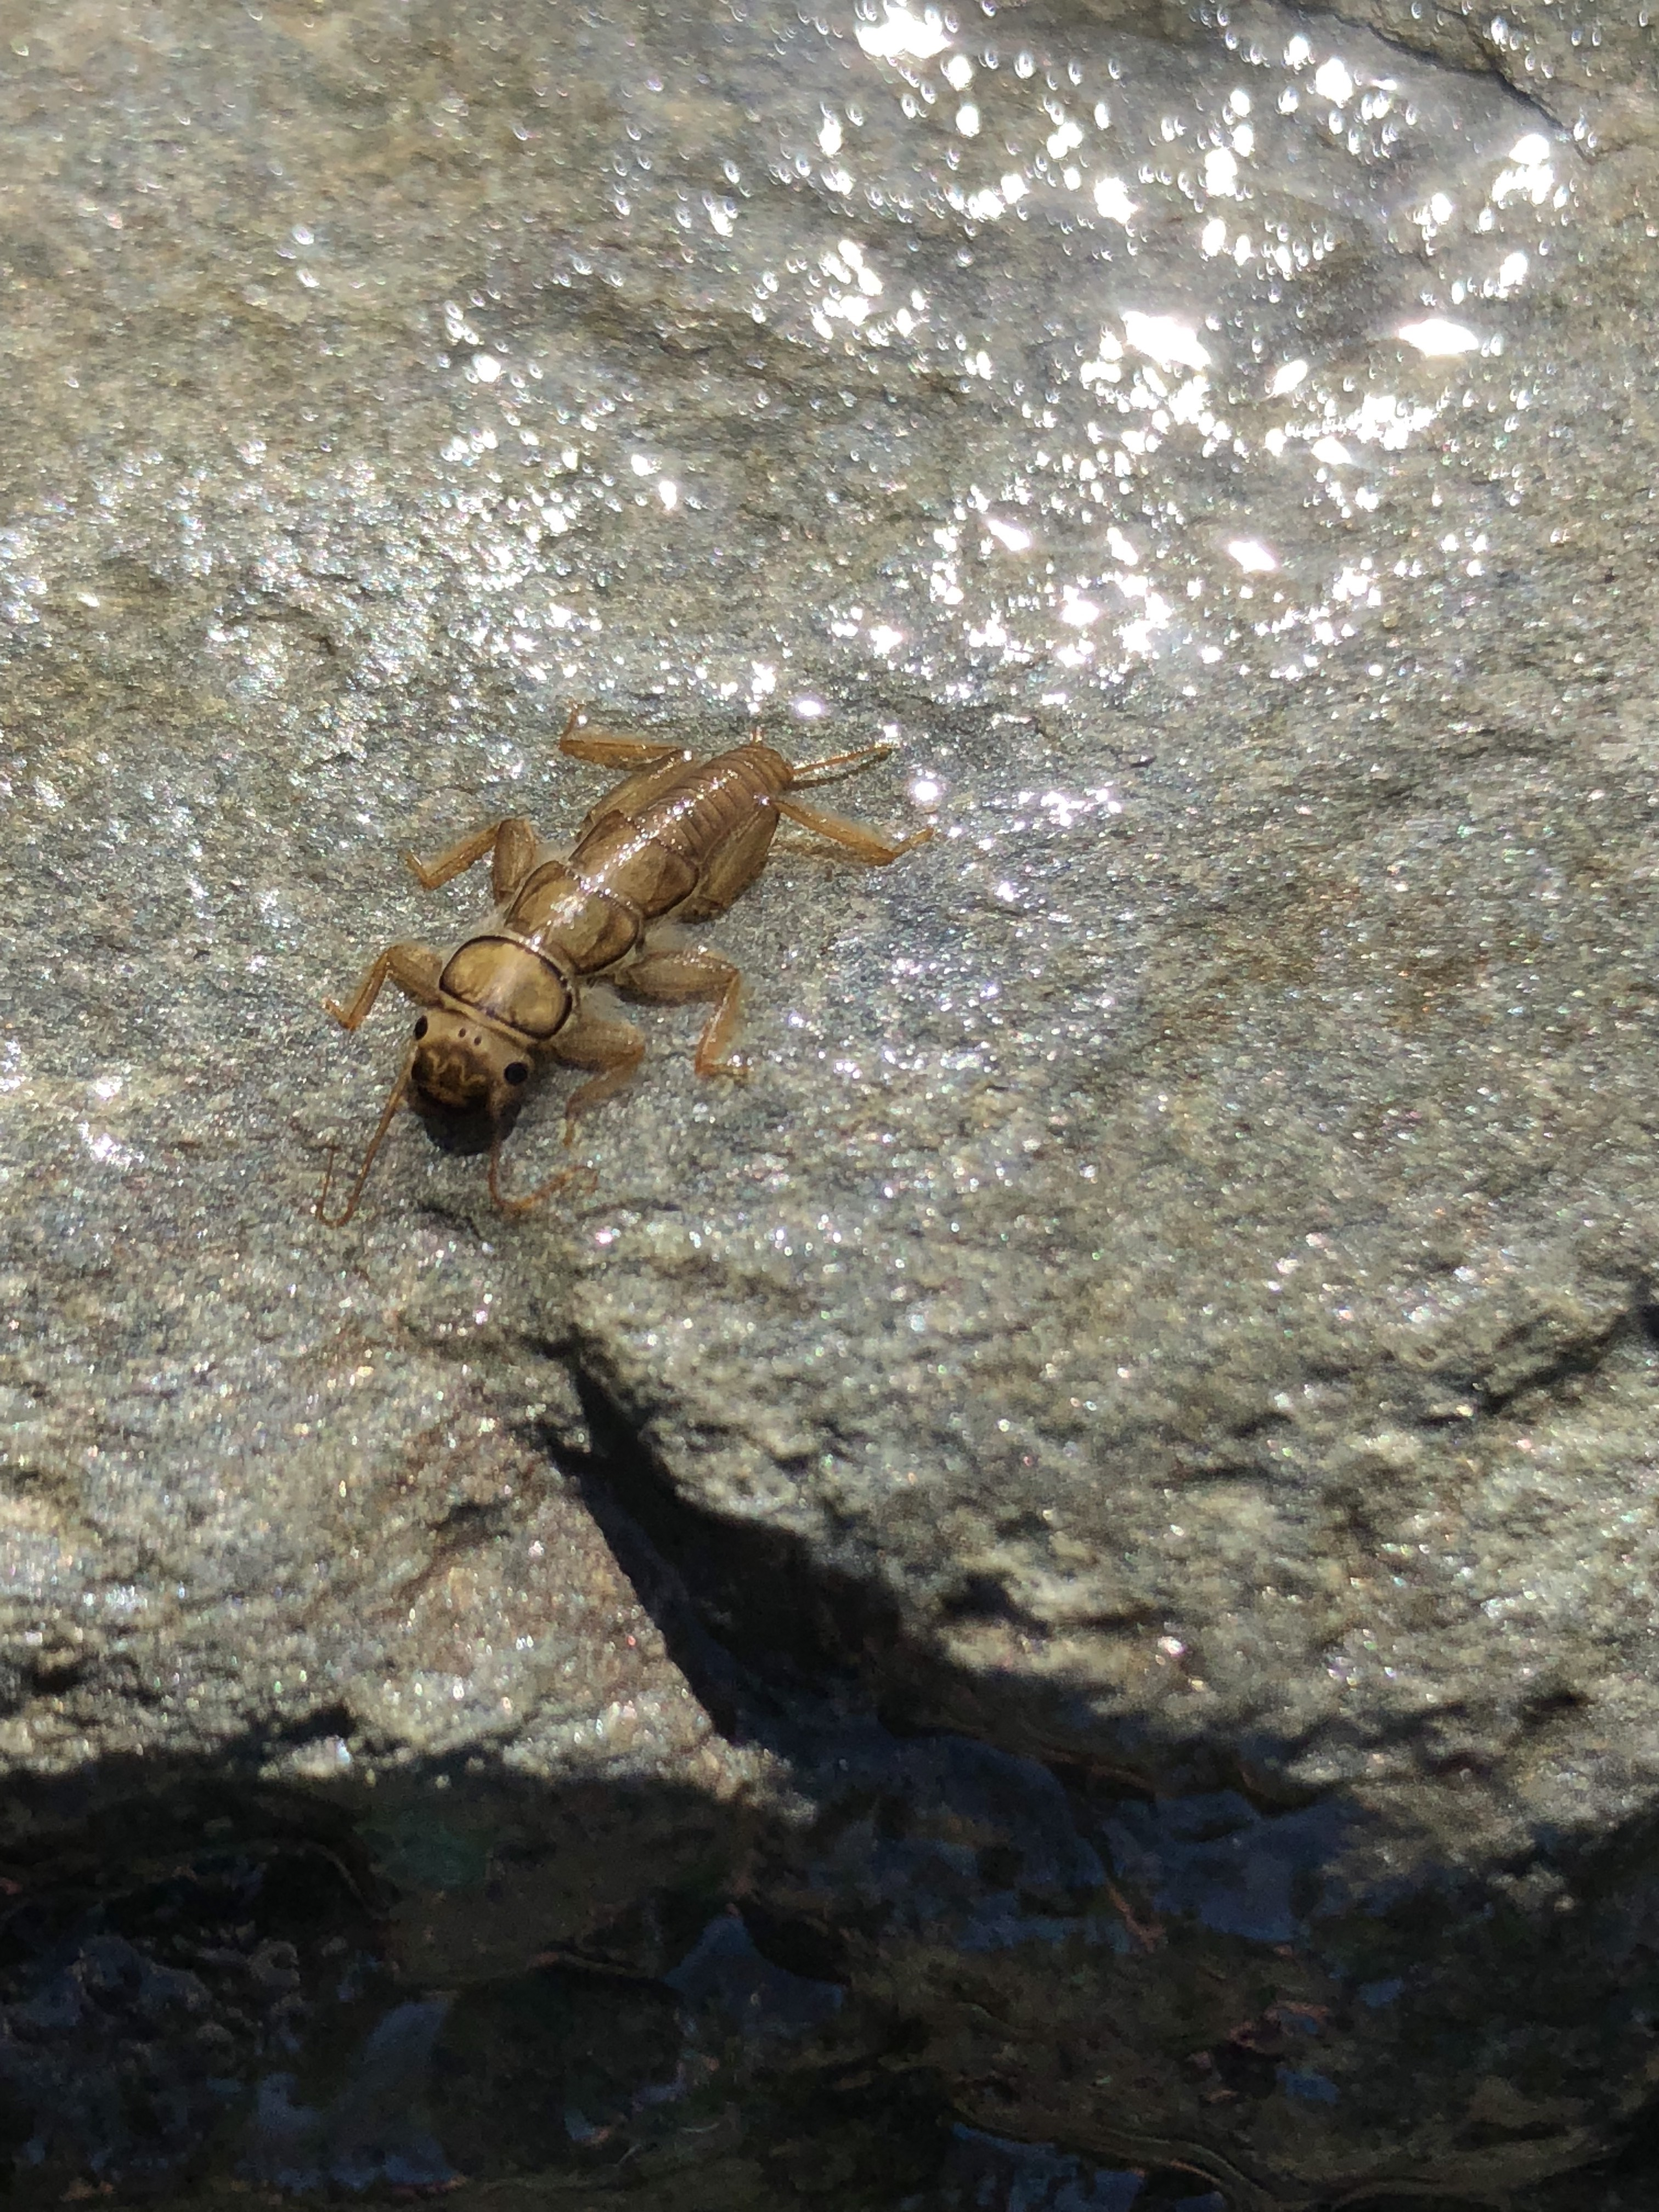
\includegraphics[width=1\textwidth]{imagenes/testAlpha/5.JPG}
					\caption{Foto real del insecto \textit{Plecoptero}}
		\end{figure}
		\begin{figure}[H]
			\centering
				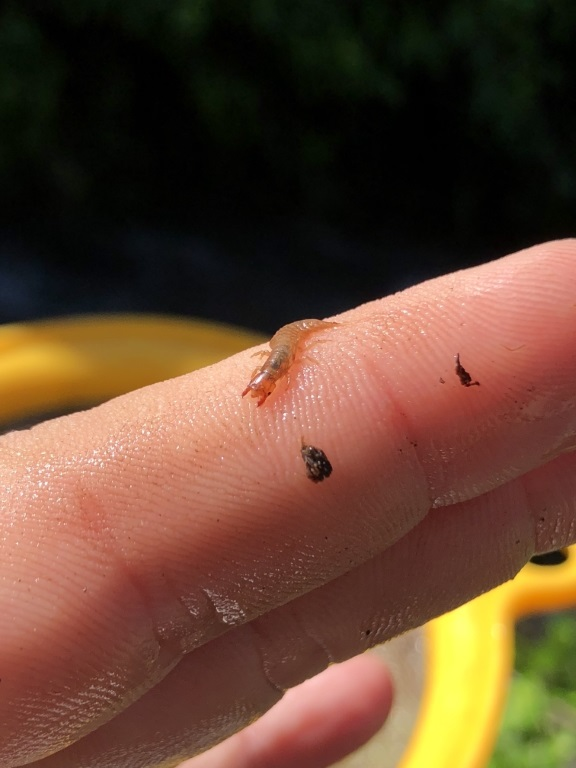
\includegraphics[width=1\textwidth]{imagenes/testAlpha/6.JPG}
					\caption{Foto real del insecto \textit{Patudo}}
		\end{figure}
		
	\subsection{Prueba Beta}

		Esta prueba se lleva a cabo en uno o más lugares de clientes, por los usuarios finales de software. El encargado de desarrollo no está presente. El cliente registra todos los problemas (reales o imaginarios) que  encuentra durante la prueba o informa a intervalos regulares al equipo de desarrollo. Se lleva a cabo en un entorno no controlado.

		Los procedimientos de prueba se diseñaron para asegurar que se satisfacen todos los requisitos funcionales y que se alcanzan todos los requisitos de rendimiento.
		\newline

		\textbf{Pruebas realizadas:}
		
		No se realizaron las pruebas betas, sin embargo se programo una para finales de octubre del 2018, con la participación de los alumnos de escuelas rurales (usuario final del sistema).


%% Conclusiones
%%%%%%%%%%%%%%%%%%%%%%%%%%%%%%%%%%%%%%%%%%%%%%%%%%%%%%%%
%   |------------------------------------------|       %
%   | Web App embebida en dispositivos móviles |       %
%   |  para la gestión de registros sobre la   |       %
%   |   contaminación de afluentes y ríos.     |       %
%   |                                          |       %
%   |          Proyecto de graduación          |       %
%   |__________________________________________|       %
%                                                      %
%   Autores                                            %
%   -------                                            %
%                                                      %
% * Bruno, Ricardo Hugo (CX 1409686)                   %
%     rburnount@gmail.com                              %
% * Gómez Veliz, Kevin Shionen (CX 1411828)            %
%     ing.gomezvelizkevin@gmail.com                    %
%                                                      %
%   Tutor                                              %
%   -------                                            %
%                                                      %
% * Ing. Cohen, Daniel Eduardo                         %
%        dcohen.tuc@gmail.com                          %
%                                                      %
%   Cotutor                                            %
%   -------                                            %
%                                                      %
% * Ing. Nieto, Luis Eduardo                           %
%        lnieto@herrera.unt.edu.ar                     %
%                                                      %
%                                                      %
%%%%%%%%%%%%%%%%%%%%%%%%%%%%%%%%%%%%%%%%%%%%%%%%%%%%%%%%

\chapter{Conclusiones}

El desarrollo de nuestro proyecto final nos permitió poner en práctica temas que aprendimos en distintas asignaturas durante el transcurso de nuestra carrera, el aprendizaje y la experiencia de implementar nuevas tecnologías, enfrentándonos a problemas reales de diseño e integración que nos forzaron a tomar decisiones a fin de encontrar soluciones eficientes a los mismos. Además, nos dio la posibilidad de aprender a trabajar con herramientas con los cuales no estábamos familiarizados.

Con la puesta en funcionamiento de este proyecto pudimos generar un producto que
da valor agregado a la metodología de trabajo existente de los docentes de la Facultad de Ciencias Naturales e Instituto Miguel Lillo en conjunto con alumnos de escuelas rurales, que no poseen automatismo en dicha metodología, cumpliendo así, con los objetivos planteados inicialmente, obteniendo un producto seguro, escalable, de fácil mantenimiento y simple de usar.

Se logró implementar a través de Web services una comunicación eficiente con la base de datos, con mecanismos de seguridad que impiden la visualización o alteración indebida de los datos sensibles de los usuarios.

Comprendimos la importancia del uso de un desarrollo modular y orientado a objetos para la realización de proyectos flexibles, escalables, más legibles y manejables en aplicaciones actuales.

También podemos decir que este sistema queda abierto a la incorporación de futuras actualizaciones para satisfacer las necesidades de los usuarios cuando los procesos así lo requieran.

\label{chap:conclusiones}



% Glosario
\printnoidxglossary[style=altlist]


%% Bibliografía
%%%%%%%%%%%%%%%%%%%%%%%%%%%%%%%%%%%%%%%%%%%%%%%%%%%%%%%%
%   |------------------------------------------|       %
%   | Web App embebida en dispositivos móviles |       %
%   |  para la gestión de registros sobre la   |       %
%   |   contaminación de afluentes y ríos.     |       %
%   |                                          |       %
%   |          Proyecto de graduación          |       %
%   |__________________________________________|       %
%                                                      %
%   Autores                                            %
%   -------                                            %
%                                                      %
% * Bruno, Ricardo Hugo (CX 1409686)                   %
%     rburnount@gmail.com                              %
% * Gómez Veliz, Kevin Shionen (CX 1411828)            %
%     ing.gomezvelizkevin@gmail.com                    %
%                                                      %
%   Tutor                                              %
%   -------                                            %
%                                                      %
% * Ing. Cohen, Daniel Eduardo                         %
%        dcohen.tuc@gmail.com                          %
%                                                      %
%   Cotutor                                            %
%   -------                                            %
%                                                      %
% * Ing. Nieto, Luis Eduardo                           %
%        lnieto@herrera.unt.edu.ar                     %
%                                                      %
%                                                      %
%%%%%%%%%%%%%%%%%%%%%%%%%%%%%%%%%%%%%%%%%%%%%%%%%%%%%%%%

% ********* Bibliografías ********** %

\begin{thebibliography}{99}

\bibitem{software1} Craig Larman. Applying UML and Patterns second edition.

\bibitem{ionic} Documentación oficial de Ionic.(\href{https://ionicframework.com/docs/}{https://ionicframework.com/docs/})

\bibitem{cordova} Documentación oficial de Apache Cordova.(\href{https://cordova.apache.org/docs/en/latest/}{https://cordova.apache.org/docs/en/latest/})

\bibitem{express} Documentación oficial de Express.js.(\href{http://expressjs.com/}{http://expressjs.com/})

\bibitem{angular} Documentación oficial de Angular.(\href{https://angular.io/docs}{https://angular.io/docs})

\bibitem{software} Roger S. Pressman. Software Enginneering sixth edition.

\bibitem{wiki-en} Wikipedia en inglés (\href{http://en.wikipedia.org/}{http://en.wikipedia.org/}).

\bibitem{wiki-es} Wikipedia en castellano (\href{http://es.wikipedia.org/}{http://en.wikipedia.org/}).

\bibitem{wikilibroslatex} Wikilibros: Manual de \LaTeX.

\bibitem{latexcientifico} Gabriel Valiente Feruglio. Composición de textos científicos con \LaTeX. 1999.

\end{thebibliography}


\end{document}
